\documentclass[final,12pt]{colt2018} % Anonymized submission
% \documentclass[11pt]{article}

% Any additional packages needed should be included after jmlr2e.
% Note that jmlr2e.sty includes epsfig, amssymb, natbib and graphicx,
% and defines many common macros, such as 'proof' and 'example'.
%
% It also sets the bibliographystyle to plainnat; for more information on
% natbib citation styles, see the natbib documentation, a copy of which
% is archived at http://www.jmlr.org/format/natbib.pdf

\usepackage{times}

% \usepackage{fullpage}
% \usepackage{natbib}
% \usepackage{algorithm}
% \usepackage[noend]{algpseudocode}

% \usepackage{amsmath,amsthm,amsfonts,amssymb}
% \usepackage{hyperref}
% % \usepackage{jmlr2e}
% \usepackage{color}
% \usepackage{mathrsfs}
% \usepackage{mathtools}
% \usepackage{enumitem}
% \usepackage{bm}
% % \usepackage{tabularx}
% \usepackage{multirow}
% \usepackage{booktabs}
% \usepackage{makecell}
% \usepackage{graphicx}
% \usepackage{subfigure}
% \usepackage{caption}



\usepackage{algorithm}
\usepackage[noend]{algorithmic}
% \usepackage{algpseudocode}

\usepackage{amsmath}
\usepackage{amsfonts}
\usepackage{amssymb}
\usepackage{color}
\usepackage{mathrsfs}
\usepackage{enumitem}
\usepackage{bm}
\usepackage{multirow}
\usepackage{booktabs}
\usepackage{makecell}
\usepackage{graphicx}
% \usepackage{subfigure}
% \usepackage{caption}

%\usepackage{nth}
\usepackage{intcalc}

% Definitions of handy macros can go here
% \setlength\parindent{0pt}

\newcommand{\defeq}{\mathrel{\mathop:}=}
\newcommand{\red}[1]{{\color{black} #1}}
\newcommand{\praneeth}[1]{{\color{blue} PN:#1}}
\newcommand{\gd}{GD}
\newcommand{\pgd}{PGD}
\newcommand{\pagd}{PAGD}
\newcommand{\nag}{AGD}
\newcommand{\fstar}{f^*}
\newcommand{\xstar}{\x^*}
\newcommand{\nce}{NCE}

\newcommand{\vect}[1]{\ensuremath{\mathbf{#1}}}
\newcommand{\mat}[1]{\ensuremath{\mathbf{#1}}}
\newcommand{\dd}{\mathrm{d}}
\newcommand{\grad}{\nabla}
\newcommand{\hess}{\nabla^2}
\newcommand{\argmin}{\mathop{\rm argmin}}
\newcommand{\argmax}{\mathop{\rm argmax}}

\newcommand{\abs}[1]{\left|{#1}\right|}
\newcommand{\norm}[1]{\left\|{#1}\right\|}
\newcommand{\order}[1]{O\left({#1}\right)}
\newcommand{\otheta}[1]{\Theta\left({#1}\right)}
\newcommand{\otilde}[1]{\widetilde{O}\left({#1}\right)}
\newcommand{\omtilde}[1]{\widetilde{\Omega}\left({#1}\right)}
\newcommand{\fnorm}[1]{\left\|{#1}\right\|_{\text{F}}}
\newcommand{\spnorm}[2]{\left\| {#1} \right\|_{\text{S}({#2})}}
\newcommand{\sigmin}{\sigma_{\min}}
\newcommand{\tr}{\text{tr}}
\renewcommand{\det}{\text{det}}
\newcommand{\rank}{\text{rank}}
\newcommand{\logdet}{\text{logdet}}
\newcommand{\trans}{^{\top}}
\newcommand{\poly}{\text{poly}}
\newcommand{\polylog}{\text{polylog}}
\newcommand{\st}{\text{s.t.~}}
\newcommand{\proj}{\mathcal{P}}
\newcommand{\projII}{\mathcal{P}_{\parallel}}
\newcommand{\projT}{\mathcal{P}_{\perp}}

\newcommand{\Bcal}{\mathcal{B}}
\newcommand{\Z}{\mathbb{Z}}
\newcommand{\N}{\mathbb{N}}
\newcommand{\R}{\mathbb{R}}
\newcommand{\C}{\mathbb{C}}
\newcommand{\E}{\mathbb{E}}
\newcommand{\Var}{\text{Var}}

\newcommand{\iol}{improve or localize}

\newcommand{\fracpar}[2]{\frac{\partial #1}{\partial  #2}}

\newcommand{\A}{\mat{A}}
\newcommand{\B}{\mat{B}}
\newcommand{\Q}{\mat{Q}}


\newcommand{\I}{\mat{I}}
\newcommand{\M}{\mat{M}}
\newcommand{\D}{\mat{D}}
\newcommand{\U}{\mat{U}}
\newcommand{\V}{\mat{V}}
\newcommand{\W}{\mat{W}}
\newcommand{\X}{\mat{X}}
\newcommand{\Y}{\mat{Y}}
\newcommand{\mSigma}{\mat{\Sigma}}
\newcommand{\mLambda}{\mat{\Lambda}}
\newcommand{\e}{\vect{e}}
\renewcommand{\u}{\vect{u}}
\renewcommand{\v}{\vect{v}}
\newcommand{\w}{\vect{w}}
\newcommand{\x}{\vect{x}}
\newcommand{\y}{\vect{y}}
\newcommand{\z}{\vect{z}}
\newcommand{\fI}{\mathfrak{I}}
\newcommand{\fS}{\mathfrak{S}}
\newcommand{\fE}{\mathfrak{E}}
\newcommand{\fF}{\mathfrak{F}}

\renewcommand{\L}{\mathcal{L}}
\renewcommand{\H}{\mathcal{H}}

\newcommand{\cn}{\kappa}
\newcommand{\nn}{\nonumber}


\newcommand{\Hess}{\nabla^2}
\newcommand{\tlO}{\tilde{O}}
\newcommand{\tlOmega}{\tilde{\Omega}}
\newcommand{\iprod}[2]{\langle #1, #2 \rangle}

% \newcommand{\M}{\mat{M}}
% \newcommand\Mmh{\mat{M}^{-1/2}}
% \newcommand{\A}{\mat{A}}
% \newcommand{\B}{\mat{B}}
% \newcommand{\C}{\mat{C}}
% \newcommand{\Et}[1][t]{\mat{E_{#1}}}
% \newcommand{\Etp}{\Et[t+1]}
% \newcommand{\Errt}[1][t]{\mat{\bigtriangleup_{#1}}}
% \newcommand\cnM{\kappa}
% \newcommand{\cn}[1]{\kappa\left(#1\right)}
% \newcommand\X{\mat{X}}
% \newcommand\fstar{f_*}
% \newcommand\Xt[1][t]{\mat{X_{#1}}}
% \newcommand\ut[1][t]{{u_{#1}}}
% \newcommand\Xtinv{\inv{\Xt}}
% \newcommand\Xtp{\mat{X_{t+1}}}
% \newcommand\Xtpinv{\inv{\left(\mat{X_{t+1}}\right)}}
% \newcommand\U{\mat{U}}
% \newcommand\UTr{\trans{\mat{U}}}
% \newcommand{\Ut}[1][t]{\mat{U_{#1}}}
% \newcommand{\Utinv}{\inv{\Ut}}
% \newcommand{\UtTr}[1][t]{\trans{\mat{U_{#1}}}}
% \newcommand\Utp{\mat{U_{t+1}}}
% \newcommand\UtpTr{\trans{\mat{U}_{t+1}}}
% \newcommand\Utptild{\mat{\widetilde{U}_{t+1}}}
% \newcommand\Us{\mat{U^*}}
% \newcommand\UsTr{\trans{\mat{U^*}}}
% \newcommand{\Sigs}{\mat{\Sigma}}
% \newcommand{\Sigsmh}{\Sigs^{-1/2}}
% \newcommand{\eye}{\mat{I}}
% \newcommand{\twonormbound}{\left(4+\DPhi{\M}{\Xt[0]}\right)\twonorm{\M}}
% \newcommand{\lamj}{\lambda_j}

% \renewcommand\u{\vect{u}}
% \newcommand\uTr{\trans{\vect{u}}}
% \renewcommand\v{\vect{v}}
% \newcommand\vTr{\trans{\vect{v}}}
% \newcommand\w{\vect{w}}
% \newcommand\wTr{\trans{\vect{w}}}
% \newcommand\wperp{\vect{w}_{\perp}}
% \newcommand\wperpTr{\trans{\vect{w}_{\perp}}}
% \newcommand\wj{\vect{w_j}}
% \newcommand\vj{\vect{v_j}}
% \newcommand\wjTr{\trans{\vect{w_j}}}
% \newcommand\vjTr{\trans{\vect{v_j}}}

% \newcommand{\DPhi}[2]{\ensuremath{D_{\Phi}\left(#1,#2\right)}}
% \newcommand\matmult{{\omega}}


% \newtheorem{theorem}{Theorem}
% \newtheorem{lemma}[theorem]{Lemma}
% \newtheorem{corollary}[theorem]{Corollary}
% \newtheorem{remark}[theorem]{Remark}
% \newtheorem{claim}{Remark}
\newtheorem*{fact}{Fact}
% \newtheorem{proposition}[theorem]{Proposition}
% \theoremstyle{definition}
% \newtheorem{definition}{Definition}
% \newtheorem{assumption}{Assumption}
% \renewcommand\theassumption{A\arabic{assumption}}

\newcommand{\g}{\bm{g}}
\newcommand{\m}{\bm{m}}

\newcommand{\ca}{\hat{c}}
\newcommand{\Ts}{T'}
\newcommand{\Tt}{T''}
\newcommand{\cb}{c_2}
\newcommand{\ugrad}{\mathscr{G}}
\newcommand{\ufun}{\mathscr{E}}
\newcommand{\uspace}{\mathscr{S}}
\newcommand{\utime}{\mathscr{T}}
\newcommand{\umom}{\mathscr{M}}

\renewcommand{\S}{\mathcal{S}}
\newcommand{\Scomp}{\mathcal{S}^c}
\newcommand{\balpha}{\bm{\alpha}}
\newcommand{\bbeta}{\bm{\beta}}
\newcommand{\bdelta}{\bm{\delta}}
\newcommand{\logterms}{\frac{d\cn}{\delta}}
\newcommand{\overh}{\ca \log(\logterms)}

\newcommand{\sigstarl}{\sigma^\star_1}
\newcommand{\sigstarr}{\sigma^\star_r}
\newcommand{\zero}{\mathbf{0}}
\newcommand{\mR}{\mat{R}}
\newcommand{\mZ}{\mat{Z}}
\newcommand{\la}{\langle}
\newcommand{\ra}{\rangle}
\newcommand{\cXstar}{\mathcal{X}^\star}
\newcommand{\cXe}{\mathcal{X}_{\text{escape}}}
\newcommand{\cXs}{\mathcal{X}_{\text{stuck}}}

\newcommand{\ball}{\mathbb{B}}
\newcommand{\EFSP}{$\epsilon$-first-order stationary point}
\newcommand{\ESSP}{$\epsilon$-second-order stationary point}
\newcommand{\ESP}{$\epsilon$-suboptimal point}

\renewcommand{\Im}{\mathrm{Im}}
\newcommand{\pmat}[1]{\begin{pmatrix} #1 \end{pmatrix}}
\newcommand{\modify}[1]{#1 '}

\newcommand{\pn}[1]{{\color{red} PN: #1}}
\newcommand{\cj}[1]{{\color{blue} CJ: #1}}
\newcommand{\cnote}{\textcolor[rgb]{1,0,0}{C: }\textcolor[rgb]{1,0,1}}

% \newcommand{\citep}{\cite}
% \newcommand{\citet}{\cite}


\begin{document}

\title[AGD Escapes Saddle Points Faster than GD]{Accelerated Gradient Descent Escapes Saddle Points Faster than Gradient Descent}

% \title{\textbf{Accelerated Gradient Descent Escapes Saddle Points Faster than Gradient Descent}}

% \author{Chi Jin \\ University of California, Berkeley \\ \texttt{chijin@cs.berkeley.edu}
% \and 
% Praneeth Netrapalli \\ Microsoft Research, India \\ \texttt{praneeth@microsoft.com}
% \and
% Michael I. Jordan \\ University of California, Berkeley \\ \texttt{jordan@cs.berkeley.edu}}

 \coltauthor{\Name{Chi Jin} \Email{chijin@cs.berkeley.edu}\\
 \addr University of California, Berkeley
 \AND
 \Name{Praneeth Netrapalli} \Email{praneeth@microsoft.com}\\
 \addr Microsoft Research India
 \AND
 \Name{Michael I. Jordan} \Email{jordan@cs.berkeley.edu}\\
 \addr University of California, Berkeley
 }

\maketitle

\begin{abstract}
% Nesterov's accelerated gradient descent (\nag), an instance of the general family of ``momentum methods,'' provably achieves faster convergence rate than gradient descent (\gd) in the convex setting. However, whether these methods are superior to~\gd~in the nonconvex setting remains open. This paper studies a simple variant of~\nag, and shows that it escapes saddle points and finds a second-order stationary point in $\tilde{O}(1/\epsilon^{7/4})$ iterations, faster than the $\tilde{O}(1/\epsilon^{2})$ iterations required by~\gd. To the best of our knowledge, this is the first Hessian-free algorithm to find a second-order stationary point faster than~\gd, and also the first single-loop algorithm with a faster rate than~\gd~even in the setting of finding a first-order stationary point. Our analysis is based on two key ideas: (1) the use of a simple Hamiltonian function, inspired by a continuous-time perspective, which~\nag~monotonically decreases per step even for nonconvex functions, and (2) a novel framework called~\emph{\iol}, which is useful for tracking the long-term behavior of gradient-based optimization algorithms. We believe that these techniques may deepen our understanding of both acceleration algorithms and nonconvex optimization.

\noindent
Nesterov's accelerated gradient descent (\nag), an instance of the general family of ``momentum methods,'' provably achieves faster convergence rate than gradient descent (\gd) in the convex setting. While these methods are widely used in modern \emph{nonconvex} applications, including training of deep neural networks, whether they are provably superior to~\gd~in the nonconvex setting remains open. This paper studies a simple variant of Nesterov's~\nag, and shows that it escapes saddle points and finds a second-order stationary point in $\tilde{O}(1/\epsilon^{7/4})$ iterations, matching the best known convergence rate, which is faster than the $\tilde{O}(1/\epsilon^{2})$ iterations required by~\gd. To the best of our knowledge, this is the first direct acceleration (single-loop) algorithm that is provably faster than GD in general nonconvex setting---all previous nonconvex accelerated algorithms rely on more complex mechanisms such as nested loops and proximal terms. Our analysis is based on two key ideas: (1) the use of a simple Hamiltonian function, inspired by a continuous-time perspective, which~\nag~monotonically decreases on each step even for nonconvex functions, and (2) a novel framework called~\emph{\iol}, which is useful for tracking the long-term behavior of gradient-based optimization algorithms. We believe that these techniques may deepen our understanding of both acceleration algorithms and nonconvex optimization.


\end{abstract}

% \thispagestyle{empty}
% \clearpage
% \newpage
% \setcounter{page}{1}

% \cnote{Think name of title, algorithm, improve or localize, negative curvature exploration}
% !TeX root = main.tex
\section{Introduction}
\label{sec:intro}
Generative models are often trained in an unsupervised fashion, fitting a model $q$ to a set of observed data $x_P \subseteq X$ drawn iid from some true distribution $p$ on $x\in X$. Now, of course $p$ may not exactly belong to family $Q$ of probability distributions being fit, whether $Q$ consists of Gaussians mixture models, Markov models, or even neural networks of bounded size. We first discuss the limitations of generative modeling without feedback, and then discuss our model and results.

%\subsection{Limitations of Generative Modeling from Positive Examples Alone}
Consider fitting a generative model on a text corpus consisting partly of poetry written by four-year-olds and partly of mathematical publications from the {\em Annals of Mathematics}. Suppose that learning to generate a poem that looks like it was written by a child was easier than learning to generate a novel mathematical article with a correct, nontrivial statement. If the generative model pays a high price for generating unrealistic examples, then it may be better off learning to generate children's poetry than mathematical publications. However, without negative feedback, it may be difficult for a neural network or any other model to know that the mathematical articles it is generating are stylistically similar to the mathematical publications but do not contain valid proofs.\footnote{This is excluding clearly fake articles published without proper review in lower-tier venues \citep{LabbeL13}.} 

As a simpler example, the classic Markovian ``trigram model'' of natural language assigns each word a fixed probability conditioned only on the previous two words. Prior to recent advances in deep learning, for decades the trigram model and its variant were the workhorses of language modeling, assigning much greater likelihood to natural language corpora than numerous linguistically motivated grammars and other attempts \citep{Rosenfeld00}. However, text sampled from a trigram is typically nonsensical, e.g., the following text was randomly generated from a trigram model fit on a corpus of text from the Wall Street Journal \citep{JurafskyM09}:
\begin{quote}
They also point to ninety nine point six billion dollars from two hundred
four oh six three percent of the rates of interest stores as Mexico and
gram Brazil on market conditions. 
\end{quote}

In some applications, like text compression using a language model \citep{WittenNC87}, maximizing likelihood is equivalent to optimizing compression. However, in many  applications involving generation, such nonsense is costly and unacceptable. Now, of course it is possible to always generate valid data by returning random training examples, but this is simply overfitting and not learning. Alternatively, one could incorporate human-in-the-loop feedback such as through crowdsourcing, into the generative model to determine what is a valid, plausible sentence.

In some domains, validity could be determined automatically. Consider a Markovian model of a well-defined concept such as mathematical formulas that compile in \LaTeX{}. Now, consider a $n$-gram Markovian character model which the probability of each subsequent character is determined by the previous $n$ characters. For instance, the expression \$\{2+\{x-y\}\$ is invalid in \LaTeX{} due to mismatched braces. For this problem, a \LaTeX{} compiler may serve as a validity oracle. Various $n$-gram models can be fit which only generate valid formulas. To address mismatched braces, for example, one such model would ensure that it always closed braces within $n$ characters of opening, and had no nested braces. While an $n$-gram model will not perfectly model the true distribution over valid \LaTeX{} formulas, for certain generative purposes one may prefer an $n$-gram model that generates valid formulas over one that assigns greater likelihood to the training data but generates invalid formulas. 

Figure \ref{fig:rectangle} illustrates a simple case of learning a rectangle model for data which is not uniform over a rectangle. A maximum likelihood model would necessarily be the smallest rectangle containing all the data, but most examples generated from this distribution may be invalid. Instead a smaller rectangle, as illustrated in the figure, may be desired.

\begin{figure}[h]\label{fig:rectangle}
\centering
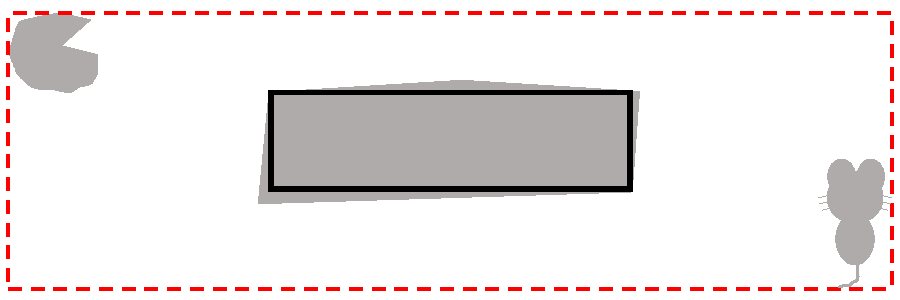
\includegraphics[width=3in]{fig.pdf}
\caption{Example where the underlying distribution $p$ is uniform over the (gray) valid regions. The solid rectangle maximizes our objective since it does not output nonsense (is supported only within the grey matter) and is closest to the $p$ (covers the maximum amount of grey matter). In contrast, the standard maximum likelihood (dashed red) rectangle must fully contain the observed samples, thus generating invalid points most of the time.  }
\end{figure}

Motivated by these observations, we evaluate a generative model $q$ on two axes. First is {\em coverage}, which is related to the probability assigned to future examples drawn from the true distribution $p$. Second is {\em validity}, defined as the probability that random examples generated from $q$ meet some validity requirement. Formally, we measure coverage in terms of a bounded {\em loss}:
$$\Loss(p,q)=\E_{x \sim p}[L(q_x)],$$
where $L:[0,1]\rightarrow [0,M]$ is a bounded decreasing function such as the capped log-loss $L(q_x)=\min(M, \log 1/q_x)$. % or $L(q_x)=\log 1/(q_x+\exp(-M))$. 
A bounded loss has the advantages of being efficiently estimable, and also it enables a model to assign 0 probability to one example (e.g., an outlier or error) if it greatly increases the likelihood of all other data. Validity is defined with respect to a set $V \subseteq X$, and $q(V)$ is the probability that a random example generated from $q$ lies within $V$. 

Clearly, there is a tradeoff between coverage and validity. We first focus on the case of (near) perfect validity. A Valid Generative Modeling (VGM) algorithm if it outputs, for a family of distributions $Q$ over $X$, if it outputs $\hat{q}$ with (nearly) perfect validity and whose loss is nearly as good as the loss of the best valid $q\in Q$. More precisely, $A$ is a VGM learner of $Q$ if for any nonempty valid subset $V \subseteq X$, any probability distribution $p$ over $V$, and any $\eps>0$, $A$ uses $n$ random samples from $p$ and makes $m$ membership oracle calls to $V$ and outputs a distribution $\hat{q}$ such that, $$\Loss(p, \hat{q}) \leq \min_{q \in Q: q(V)=1}\Loss(p,q) + \eps ~\text{ and }~\hat{q}(V)\geq 1-\eps.$$ 
We aim for our learner to be sample and query efficient, requiring that $n$ and $m$ are polynomial in $M, 1/\eps$ and a measure of complexity of our distribution class $Q$.
Furthermore, we would like our algorithms to be computationally efficient, with a runtime polynomial in the size of the data, namely the $n + m$ training examples. 
A more formal description of the problem is available in Section~\ref{sec:problem}.

$A$ is said to be {\em proper} if it always outputs $\hat{q}\in Q$ and {\em improper} otherwise.
In Section~\ref{sec:impossibility}, we first show that efficient proper learning for VGM is impossible. This is an information-theoretic result, meaning that even given infinite runtime and positive samples, one still cannot solve the VGM problem. Interestingly, this is different from binary classification, where it is possible to statistically learn from iid examples without a membership oracle.

Our first main positive result is an efficient (improper) learner for VGM. The algorithm relies on a subroutine that solves the following {\em Generative Modeling with Negatives} (GMN) problem: given sets $X_P, X_N \subset X$ of positive and negative examples, find the probability distribution $q \in Q$ which minimizes $\sum_{x \in X_P} L(q(x))$ subject to the constraint that $q(X_N)=0$. For simplicity, we present our algorithm for the case that the distribution family $Q$ is finite, giving sample and query complexity bounds that are logarithmic in terms of $|Q|$. However, as we show in Section~\ref{sec:infinite-families}, all of our results extend to infinite families $Q$. It follows that if one has a computationally efficient algorithm for the GMN problem for a distribution family $Q$, then our reduction gives a computationally efficient VGM learning algorithm for $Q$.

Our second positive result is an algorithm that minimizes $\Loss(p,q)$ subject to a relaxed validity constraint comparing against the optimal distribution that has validity $q(V)$ at least $1-\alpha$ for some $\alpha>0$. We show in Section~\ref{sec:partial-validity} that even in this more general setting, it is possible to obtain an algorithm that is statistically efficient but may not be computationally efficient. An important open question is whether there exists a computationally efficient algorithm for this problem when given access to an optimization oracle, as was the case for our algorithm for VGM.

\subsection{Related Work}
\cite{KearnsMRRSS94} showed how to learn distributions from positive examples in the realizable setting, i.e., where the true distribution is assumed to belong to the class being learned. In the same sense as their work is similar to PAC learning \citet{Valiant84} of distributions, our work is like agnostic learning \citet{KearnsSS94} in which no assumption on the true distribution is made. 

Generative Adversarial Networks (GANs)~\cite{GoodfellowPMXWOCB14} are an approach for generative modeling from positive examples alone, in which a generative model is trained against a discriminator that aims to distinguish real data from generated data. In some domains, GANs have been shown to outperform other methods at generating realistic-looking examples. Several shortcomings of GANs have been observed \citet{AroraRZ18}, and GANs are still subject to the theoretical limitations we argue are inherent to any model trained without a validity oracle. 

In supervised learning, there is a rich history of learning theory with various types of queries, including membership which are not unlike our (in)validity oracle. Under various assumptions, queries have been shown to facilitate the learning of complex classes such as finite automata \citet{Angluin88} and DNFs \citet{Jackson97}. See the survey of \cite{Angluin92} for further details.  Interestingly, \cite{Feldman09} has shown that for agnostic learning, i.e., without making assumptions on the generating distribution, the addition of membership queries does not enhance what is learnable beyond random examples alone. 
Supervised learning also has a large literature around active learning, showing how the ability to query examples reduces the sample complexity of many algorithms. See the survey of \cite{Hanneke14}. Note that the aim here is typically to save examples and not to expand what is learnable.
 
More sophisticated models, e.g., involving neural networks, can mitigate the invalidity problem as they often generate more realistic natural language and have even been demonstrated to generate \LaTeX{} that nearly compiles \citep{Karpathy15} or nearly valid Wikipedia markdown. However, longer strings generated are unlikely to be valid. For example, \cite{Karpathy15} shows generated markdown which includes:
\begin{quote}
==Access to ''rap===
The current history of the BGA has been [[Vatican Oriolean Diet]], British Armenian, published in 1893.  While actualistic such conditions such as the [[Style Mark Romanians]] are still nearly not the loss.
\end{quote}

Even ignoring the mismatched quotes and equal signs, note that this example has two so-called ``red links'' to two pages that do not exist. Without checking, it was not obvious to us whether or not Wikipedia had pages titled {\em Vatican Oriolean Diet} or {\em Style Mark Romanians}. In some applications, one may or may not want to disallow red links. In the case that they are considered valid, one may seek a full generative model of what might plausibly occur inside of brackets, as the neural network has learned in this case. If they are disallowed, a model might memorize links it has seen but not generate new ones. A validity oracle can help the learner identify what it should avoid generating.

 In practice, \cite{KusnerPH17} discuss how generative models from neural networks (in particular autoencoders) often generate invalid sequences. 
\cite{JanzWPKH18} learn the validity of examples output by a generative model using oracle feedback. 

\section{Related Work} \label{sec:related}


Mixtures of Linear Regressions is a popular mixture model (e.g.,~\citep{de1989mixtures,grun2007applications} and \citep{faria2010fitting}), also known as Hierarchical Mixture of Experts in~\citep{jordan1994hierarchical} in the machine learning community. 
It has many applications, such as trajectory clustering~\citep{gaffney1999trajectory} and phase retrieval~\citep{balakrishnan2017statistical}, and has as special cases some popular models, such as piecewise linear regression and locally linear regression.

Learning MLR in general is NP-hard~\citep{yi2014alternating}. Recent interests have been in providing various efficient algorithms for recovering the parameters in MLR under assumptions about the data generation model~\citep{chaganty2013spectral,chen2014convex,yi2014alternating,zhong2016mixed,klusowski2017estimating}. 
%These results assumes the data $x$ in different components are all from the standard Gaussians. 
They are either under restricted assumptions about the data (mixtures of two component or $x$ all from the standard Gaussian)~\citep{chen2014convex,yi2014alternating,balakrishnan2017statistical,klusowski2017estimating}, or have high sample or computational complexity~\citep{chaganty2013spectral,sedghi2016provable}. 

Some works study specific algorithms for the problem, such as  the Expectation Maximization (EM) algorithm~\citep{khalili2007variable,yi2014alternating,balakrishnan2017statistical,klusowski2017estimating}. It is known that without careful initialization EM is only guaranteed to have local convergence~\citep{klusowski2017estimating}. A grid search method for initialization is proposed in~\citep{yi2014alternating} but is only for the two-component case. It is unclear how to generalize these guarantees to our more general setting where the data $x$ from different components are from different Gaussians.
Moreover, EM also often suffers from a high computational cost.
%, for example, exact optimization in each EM step has $O(d^2 N + d^3)$ complexity. 

Another line of works used tensor methods for MLR~\citep{chaganty2013spectral,sedghi2016provable}. The third-order moment is directly estimated in~\citep{chaganty2013spectral} using samples from Gaussian distribution and is estimated from a linear regression problem in~\citep{sedghi2016provable}. A significant drawback of tensor methods is high sample and computational complexity, due to the high cost in estimating and operating over the tensors. 

\citep{chen2014convex} provided a convex relaxation formulation and showed that their algorithm is information-theoretically optimal. However, it is only for the two-component case and suffers from high computational cost in nuclear norm minimization. 

\citep{zhong2016mixed} provided a non-convex objective function that is locally strongly convex in the neighborhood of the ground truth, and proposed to first use a tensor method for initialization and then optimize the provided objective, achieving a global convergence guarantee. The overall algorithm is fixed parameter tractable in the number of components, and achieves nearly optimal sample and time complexity when this parameter is constant. However, it requires all components have the standard Gaussian distribution. It is unclear how to generalize the result to our more general setting where the data $x$ from different components are from different Gaussians. Furthermore, due to the tensor initialization, the algorithm needs complicated assumptions on the moments, while our only essential assumption is that the weight parameters can be separated, which is much simpler and more general (in fact, it is essentially necessary for obtaining any recovery guarantees).

\citep{yi2016solving} gives an improved way of using the tensor method plus alternative minimization so the sample complexity linearly depend on $d$. However, their algorithm  requires that all the data are from the standard Gaussian, and the sample complexity also depends on the minimal singular value of certain moment matrix, which can be $ \Delta^{\Omega(k)}$ small in our setting. 

%!TEX root = main.tex

\subsection{Main Techniques}\label{sec:tech}
Our results rely on the following three key ideas. To the best of our knowledge, the first two are novel, while the third one was delineated in~\citet{jin2017escape}.

\textbf{Hamiltonian:}
A major challenge in analyzing momentum-based algorithms is that the objective function does not 
decrease monotonically as is the case for~\gd. To overcome this in the convex setting, several Lyapunov functions have been proposed~\citep{wilson2016lyapunov}. However these Lyapunov functions involve the 
global minimum $\x^\star$, which cannot be computed by the algorithm, and is thus of limited value in
the nonconvex setting. A key technical contribution of this paper is the design of a function 
which is both computable and tracks the progress of~\nag. The function takes the form of a
Hamiltonian:
\begin{equation}\label{eqn:hamiltonian}
	E_t \defeq f(\x_t) + \frac{1}{2\eta} \norm{\v_t}^2;
\end{equation}
i.e., a sum of potential energy and kinetic energy terms.  It is monotonically decreasing
in the continuous-time setting \red{\emph{regardless of the convexity of $f(\cdot)$}}. This is \emph{not} the case in general in the discrete-time setting,
a fact which requires us to incorporate the~\nce~step---see Section~\ref{sec:hamiltonian} for more details. \red{We note that monotonic decrease of the Hamiltonian, by itself, does not give any convergence rate, which brings us to our second key technical contribution.}
% \red{It is monotonically decreasing for standard \nag~unless large negative curvature is observed at $\x_t$ along $\v_t$ direction}




% \red{In the continuous time setting (i.e., when the stepsize is infinitesimally small), it is monotonically decreasing \emph{regardless of the convexity of $f(\cdot)$}. In the discrete setting however, the Hamiltonian might not decrease if $f(\cdot)$ has a large negative curvature at $x_t$ in the $v_t$ direction (formally line $8$ of Algorithm~\ref{algo:PAGD}). However, handling this situation is easy and is accomplished by the~\nce~step. The challenging case is when $f(\cdot)$ does not have large negative curvature at $x_t$ in the $v_t$ direction. Here, we have decrease of Hamiltonian but that by itself does not give improved convergence rates. This brings us to our second key technical contribution.
% }

%This is \emph{not} the case in general in the discrete-time setting,
%a fact which requires us to incorporate the~\nce~step.

\textbf{Improve or localize:}
%Another key technical contribution of
This paper formalizes a simple but powerful framework 
for analyzing long-term behavior of nonconvex optimization algorithms.  This framework requires us to show that for a given algorithm, \emph{either the algorithm makes significant progress or the iterates do not move much}.
% lie in a small ball around the starting point}. 
We call this the~\emph{improve-or-localize}~phenomenon. For instance, when progress is measured 
by function value, it is easy to show that for~\gd, with proper choice of learning rate, we have: 
$$ \frac{1}{2\eta} \sum_{\tau=0}^{t-1} \norm{\x_{\tau+1} - \x_\tau}^2 \le f(\x_0) - f(\x_t).$$
% which means either function decreases a lot, or the sum of distance square is upper-bounded. 
For~\nag, a similar lemma can be shown by replacing the objective function with the Hamiltonian 
(see Lemma \ref{lem:energy_nonconvex}).  Once this phenomenon is established, we can conclude 
that if an algorithm does not make much progress, it is localized to a small ball, and we can then 
approximate the objective function by either a linear or a quadratic function (depending on smoothness 
assumptions) in this small local region. Moreover, an upper bound on 
$\sum_{\tau=0}^{t-1} \norm{\x_{\tau+1} - \x_\tau}^2$ lets us conclude that iterates do not 
oscillate much in this local region (oscillation is a unique phenomenon of momentum algorithms 
as can be seen even in the convex case).  This gives us better control of approximation error.
% \cnote{decide whether say with this technique it's easy to recover Lan's result of AGD here.}

% \pn{Better name?} Let us illustrate this for the simple case of gradient descent,
% \begin{align*}
%     x_{t+1} = x_t - \eta \nabla f(x_t),
% \end{align*}
% where $x_t$ is the current iterate, $x_{t+1}$ is the next iterate, $\eta$ is the step size and $\nabla f(x_t)$ is the gradient of the function at $x_t$. Given that the function is $\ell$-smooth i.e., $\norm{\nabla f(x) - \nabla f(y)} \leq \ell \norm{x-y}$, we see that
% \begin{align*}
%     f(x_{t+1}) &= f(x_t - \eta \nabla f(x_t))
% %   = f(x_t) - \iprod{\nabla f(\widetilde{x})}{\eta \nabla f(x_t)}
%     \leq f(x_t) - \eta\left(1-\eta \ell\right) \norm{\nabla f({x_t})}^2,
% \end{align*}
% where we used mean value theorem and the smoothness of $f$. This can be written equivalently as $f(x_{t+1}) \leq f(x_{t}) - \frac{1-\eta \ell}{\eta} \norm{x_{t+1}-x_t}^2$. Taking a telescopic sum over $t$, we obtain
% \begin{align*}
%     f(x_{t+1}) \leq f(x_0) - \frac{1-\eta \ell}{\eta} \cdot \sum_{i=0}^{t} \norm{x_{i+1} - x_i}^2 \leq f(x_0) - \frac{1-\eta \ell}{\eta} \cdot \frac{\norm{x_{t+1} - x_0}^2}{t},
% \end{align*}
% where we use Cauchy-Schwartz inequality in the last step. This can be rewritten as
% \begin{align*}
%     {\norm{x_{t+1} - x_0}^2} \leq \frac{\eta t}{1-\eta \ell} \cdot \left(f(x_0) - f(x_{t+1})\right),
% \end{align*}
% establishing~\iol~phenomenon for~\gd.

% Once we establish~\iol~phenomenon for a given algorithm, we can conclude that if the algorithm is not making progress in function value, it is localized to a small ball $\Bcal$ around the starting point. We then approximate the function by either a linear or quadratic (depending on smoothness assumptions) in the small local region $\Bcal$ and analyze the performance of algorithm on the linear/quadratic approximation keeping track of the approximation error as well.

\textbf{Coupling sequences for escaping saddle points:} When an algorithm arrives in the neighborhood of a strict saddle point, where $\lambda_{\min}(\hess f(\x)) <0$, all we know is that there exists a direction of
escape (the direction of the minimum eigenvector of $\hess f(\x)$); denote it by $\e_{\text{esc}}$. To avoid such points, the algorithm randomly perturbs the current iterate uniformly in a small ball, and runs~\nag~starting from this point $\tilde{\x}_0$. %sampling uniform from a ball.
As in~\cite{jin2017escape}, we can divide this ball into a ``stuck region,'' 
$\mathcal{X}_{\text{stuck}}$, starting from which~\nag~does not escape the saddle 
quickly, and its complement from which~\nag~escapes quickly. In order to show 
quick escape from a saddle point, we must show that the volume of $\mathcal{X}_{\text{stuck}}$ 
is very small compared to that of the ball. Though $\mathcal{X}_{\text{stuck}}$ may 
be without an analytical form, one can control the rate of escape by studying 
two~\nag~sequences that start from two realizations of perturbation, $\tilde{\x}_0$ and $\tilde{\x}'_0$, 
which are separated along $\e_{\text{esc}}$ by a small distance $r_0$. In this case, 
at least one of the sequences escapes the saddle point quickly, which proves that the 
width of $\mathcal{X}_{\text{stuck}}$ along $\e_{\text{esc}}$ can not be greater than 
$r_0$, and hence $\mathcal{X}_{\text{stuck}}$ has small volume.



%  and would like to show that with high probability, the perturbation gives us a better perturbed point $\tilde{\x}_0$, which leads to faster escaping saddle point by running AGD starting at $\tilde{\x}_0$.





% The key requirement for implementing this framework is establishing~\iol~phenomenon for the given algorithm -- in our case,~\nag. One of the key technical contributions of this paper is in designing an energy function for~\nag~and using it to establish~\iol~phenomenon.

% \pn{Put lemma here on energy function and~\iol}

% \pn{Put some stress on novelty of energy function?}
% Once~\iol~phenomenon is established, we approximate the function locally by a quadratic, and analyze~\nag's performance on this quadratic. Bounding approximation errors introduced here turns out to be technically quite challenging. Bulk of this paper is devoted to doing just that.

% We would like to reiterate that while the~\iol~framework as well as establishing this phenomenon for~\nag~are quite simple, they are quite powerful and yield short and simple proofs of some well-known existing results e.g., convergence rate of~\nag~to first order stationary points originally proved in~\cite{ghadimi2016accelerated}. See Section~\ref{sec} for details. We believe that~\iol~is the right framework for nonconvex optimization and will help push its boundaries.\pn{Something better in the last sentence?}


%!TEX root = main.tex

\section{Preliminaries}
In this section, we will review some well-known results on~\gd~and~\nag~in the strongly convex setting, 
and existing results on convergence of~\gd~to second-order stationary points. 
% The pseudocode for these algorithms is given in Algorithms~\ref{algo:gd} and~\ref{algo:AGD} respectively.

% \cnote{Show gradient descent in equation}

\subsection{Notation}
Bold upper-case letters ($\A, \B$) denote matrices and bold lower-case letters ($\x, \y$) denote vectors. 
For vectors $\norm{\cdot}$ denotes the $\ell_2$-norm. For matrices, $\norm{\cdot}$ denotes the spectral norm and $\lambda_{\min}(\cdot)$ denotes the minimum eigenvalue.
For $f: \R^d \rightarrow \R$, $\grad f(\cdot)$ and  $\hess f(\cdot)$ denote its gradient and Hessian respectively, and $f^\star$ denotes its global minimum.
% Other than Section \ref{sec:related}, 
We use $O(\cdot), \Theta(\cdot), \Omega(\cdot)$ to hide absolute constants, and $\tilde{O}(\cdot), \tilde{\Theta}(\cdot), \tilde{\Omega}(\cdot)$ to hide absolute constants and polylog factors for all problem parameters. 
% \praneeth{I think it will be cleaner to make the dependence on smoothness parameters in Table~\ref{tab:main} and edit this statement} \jccomment{Then I also need to add function value dependence, maybe too complicated to compare}.\praneeth{The issue with this is that $O()$ is not just hiding constants but also problem dependent parameters. May be mention this explicitly in the caption to the table.} 
% We let $\ball^{(d)}_\x(r)$ denote the d-dimensional ball centered at $\x$ with radius $r$; when it is clear from context, we simply denote it as $\ball_\x(r)$. We use $\proj_{\mathcal{X}}(\cdot)$ to denote projection onto the set $\mathcal{X}$. Distance and projection are always defined in a Euclidean sense.


% \pn{Talk about ignoring $\log d$ factors in notation.}

\subsection{Convex Setting}\label{sec:prelim_convex}
% \begin{figure}[t]
% \begin{minipage}{0.5\textwidth}
% 	\begin{algorithm}[H]
% 	\caption{\gd($\x_0, \eta$)}\label{algo:gd}
% 	\begin{algorithmic}[1]
% 		\For{$t = 0, 1, \ldots, T $}
% 		\State $\x_{t+1} \leftarrow \x_t - \eta \grad f (\x_t)$
% 		\EndFor
% 		\State \textbf{return} $\x_T$
% 	\end{algorithmic}
% 	\end{algorithm}
% 	\vspace{0.5cm}
% \end{minipage}
% \begin{minipage}{.5\textwidth}

% \end{minipage}
% \end{figure}
To minimize a function $f(\cdot)$,~\gd ~performs the following sequence of steps:
\begin{equation*}
\x_{t+1} = \x_{t}- \eta \grad f(\x_t).
\end{equation*}
The suboptimality of~\gd~and the improvement achieved by~\nag~can be clearly illustrated for the case of smooth and strongly convex functions. %The definitions of smoothness and strong convexity are as follows.
\begin{definition}\label{def:smooth}
A differentiable function $f(\cdot)$ is \textbf{$\ell$-smooth (or $\ell$-gradient Lipschitz)} if:
\begin{equation*}
\norm{\grad f(\x_1) - \grad f(\x_2)} \le \ell \norm{\x_1 - \x_2} \quad \forall \; \x_1, \x_2.
\end{equation*}
\end{definition}
\noindent
The gradient Lipschitz property asserts that the gradient can not change too rapidly in a small local region.
\begin{definition}\label{def:convex}
A twice-differentiable function $f(\cdot)$ is \textbf{$\alpha$-strongly convex} if
$\lambda_{\min}(\hess f(\x)) \ge \alpha, \;  \forall \; \x$.
% $f(\x_2) \ge f(\x_1) + \la \grad f(\x_1), \x_2 - \x_1 \ra + \frac{\alpha}{2}\norm{\x_2 - \x_1}^2, \quad \forall \; \x_1, \x_2.$
\end{definition}
Let $\fstar \defeq \min_{\y}f(\y)$. A point $\x$ is said to be \textbf{$\epsilon$-suboptimal} if $f(\x)  \le  \fstar + \epsilon$. The following theorem gives the convergence rate of GD and AGD for smooth and strongly convex functions.
\begin{theorem}[\cite{nesterov2004introductory}]\label{thm:gd_convex}
Assume that the function $f(\cdot)$ is $\ell$-smooth and $\alpha$-strongly convex. Then, for any $\epsilon>0$,
the iteration complexities to find an $\epsilon$-suboptimal point are as follows:
\begin{itemize}
\item GD with $\eta  = 1/\ell$: \quad $O((\ell/\alpha) \cdot \log ((f(\x_0) - \fstar)/\epsilon))$
\item AGD (Algorithm~\ref{algo:AGD}) with $\eta = 1/\ell$ and $\theta = \sqrt{\alpha/\ell}$:
\quad$O(\sqrt{\ell/\alpha} \cdot \log ((f(\x_0) - \fstar)/\epsilon))$.
\end{itemize}
% ~\gd~with $\eta = \frac{1}{\ell}$ will output an \ESP ~in iterations:
% \begin{equation*}
% O\left(\frac{\ell}{\alpha}\log \frac{f(\x_0) - \fstar}{\epsilon}\right).
% \end{equation*}
\end{theorem}

The number of iterations of GD depends linearly on the ratio $\ell/\alpha$, which is called the condition number of $f(\cdot)$ since $\alpha \I \preceq\hess f(\x) \preceq \ell \I $. Clearly $\ell \geq \alpha$ and hence condition number is always at least one. Denoting the condition number by ${\cn}$, we highlight two important aspects of~\nag: (1) the momentum parameter satisfies $\theta = 1/\sqrt{\cn}$ and (2) \nag~improves upon GD by a factor of $\sqrt{\cn}$. 
% The following theorem gives the convergence rate of~\nag~for these problems.
% \begin{theorem}[\cite{nesterov2004introductory}]\label{thm:agd_convex}
% Assume that the function $f(\cdot)$ is $\ell$-smooth and convex. Then, for any $\epsilon>0$,~\nag~with $\eta = \frac{1}{\ell}$ and $\theta = \Theta(\sqrt{\frac{\alpha}{\ell}}) $ will output an~\ESP~in iterations:
% \begin{equation*}
% O\left(\sqrt{\frac{\ell}{\alpha}}\log \frac{f(\x_0)-\fstar }{\epsilon}\right).
% \end{equation*}
% \end{theorem}
% \noindent
% Note that the rate here improves upon that of~\gd~by a factor of $\sqrt{\frac{\ell}{\alpha}}$ i.e., squareroot of the condition number.
%say something about condition number.

\subsection{Nonconvex Setting}
For nonconvex functions finding global minima is NP-hard in the worst case. The best one can hope for in this setting is convergence to stationary points. There are various levels of stationarity.
\begin{definition}
$\x$ is an \textbf{\EFSP} of function $f(\cdot)$ if $\norm{\grad f(\x)} \le \epsilon$.
\end{definition}
\noindent
As mentioned in Section~\ref{sec:intro}, for most nonconvex problems encountered in practice, a majority of first-order stationary points turn out to be saddle points. Second-order stationary points require not only zero gradient, but also positive semidefinite Hessian, ruling out most saddle points.
%Therefore, this paper focus on finding second-order stationary point.
%In order to discuss Hessian-related properties meaningfully, we first need to assert Hessian smoothness condition.
Second-order stationary points are meaningful, however, only when the Hessian is continuous.
% second order stationary points which means that in addition to being first order stationary points, the Hessian at these points is almost positive semidefinite. This is meaningful only if the Hessian does not change arbitrarily (and perhaps have large negative eigenvalues) in a small neighborhood around this point. In other words, finding second order stationary points is meaningful only if the Hessian is continuous.
%\cnote{Should we talk the case where gradient is Lipschitz but Hessian is not?}
% \begin{theorem}[\citep{nesterov1998introductory}]\label{thm:grad_smooth}
% Assume that the function $f(\cdot)$ is $\ell$-smooth. Then, for any $\epsilon>0$, gradient descent will output an \EFSP ~in iterations:
% \begin{equation*}
% \frac{\ell(f(\x_0) - f^\star)}{\epsilon^2}.
% \end{equation*}
% \end{theorem}
\begin{definition}\label{def:HessianLip}
A twice-differentiable function $f(\cdot)$ is \textbf{$\rho$-Hessian Lipschitz} if:
\begin{equation*}
\norm{\hess f(\x_1) - \hess f(\x_2)} \le \rho \norm{\x_1 - \x_2} \quad \forall \; \x_1, \x_2.
\end{equation*}
\end{definition}
%\noindent
% For Hessian Lipschitz functions, we recall the definition of second order stationary points from~\cite{nesterov2006cubic}.
\begin{definition}[\cite{nesterov2006cubic}]\label{def:SOSP}
For a $\rho$-Hessian Lipschitz function $f(\cdot)$, $\x$ is an \textbf{\ESSP} if:
% $\norm{\grad f(\x)} \le \epsilon$ and $\lambda_{\min}(\hess f(\x)) \ge - \sqrt{\rho \epsilon}$.
\begin{equation*}
\norm{\grad f(\x)} \le \epsilon \quad\text{and}\quad \lambda_{\min}(\hess f(\x)) \ge - \sqrt{\rho \epsilon}.
\end{equation*}
\end{definition}
\noindent
The following theorem gives convergence rate of perturbed~\gd~to second-order stationary points.
%See~\cite{jin2017escape} for a detailed description of the algorithm.
\begin{theorem}[\citep{jin2017escape}]\label{thm:perturbed_GD}
Assume that the function $f(\cdot)$ is $\ell$-smooth and $\rho$-Hessian Lipschitz. Then, for any $\epsilon>0$, perturbed GD outputs an \ESSP ~w.h.p in iterations:
\begin{equation*}
\otilde{\frac{\ell(f(\x_0) - \fstar)}{\epsilon^2}}.
\end{equation*}
\end{theorem}
\noindent
Note that this rate is essentially the same as that of~\gd~for convergence to first-order stationary points. In particular, it only has polylogarithmic dependence on the dimension.

%!TEX root = main.tex

\section{Main Result}\label{sec:results}

% \begin{algorithm}[t]
% \caption{Perturbed AGD with Negative Curvature Exploration
% ($\x_0, \eta, \theta, r, s$)}\label{algo:PAGD}
% \begin{algorithmic}[1]
% \State $\v_0 \leftarrow 0$
% \For{$t = 0, 1, \ldots, T $}
% \If{perturbation condition holds}
% \State $\x_t \leftarrow \x_t + \xi_t \qquad \xi_t \sim \text{Unif}\left(B_0(r)\right)$
% \EndIf
% \State $\y_{t} \leftarrow \x_{t} + (1-\theta) \v_t$
% \State $(\x_{t+1}, ~\v_{t+1}) \leftarrow (\y_t - \eta \grad f (\y_t), ~\x_{t+1} - \x_t)$
% \If{certificate Eq.\eqref{eq:certificate} is false}
% \State $(\x_{t+1}, \v_{t+1}) \leftarrow $ Negative-Curvature-Exploitation($\x_t, \v_t, s$)
% \EndIf
% \EndFor
% \State \textbf{return} $\x_T$
% \end{algorithmic}
% \end{algorithm}





\begin{algorithm}[t]
\caption{Negative Curvature Exploitation$\left(\x_t, \v_t, s\right)$}\label{algo:NCE}
\begin{algorithmic}[1]
\IF{$\norm{\v_t} \ge s$}
\STATE $\x_{t+1} \leftarrow \x_t$;
\ELSE
\STATE $\delta = s\cdot \v_t/\norm{\v_t}$
\STATE $\x_{t+1} \leftarrow \argmin_{\x \in \{\x_t + \delta, \x_t - \delta\}} f(\x)$
\ENDIF
\STATE \textbf{return} $(\x_{t+1}, 0)$
\end{algorithmic}
\end{algorithm}











% \begin{figure}[t]
% 	\begin{minipage}{0.48\textwidth}
% 	\begin{algorithm}[H]
% 	\caption{Perturbed AGD with Negative Curvature Exploration
% 	($\x_0, \eta, \theta, r, s$)}\label{algo:PAGD}
% 	\begin{algorithmic}[1]
% 	\State $\v_0 \leftarrow 0$
% 	\For{$t = 0, 1, \ldots, T $}
% 	\If{perturbation condition holds}
% 	\State $\x_t \leftarrow \x_t + \xi_t \qquad \xi_t \sim \text{Unif}\left(B_0(r)\right)$
% 	\EndIf
% 	\State $\y_{t} \leftarrow \x_{t} + (1-\theta) \v_t$
% 	\State $(\x_{t+1}, ~\v_{t+1}) \leftarrow (\y_t - \eta \grad f (\y_t), ~\x_{t+1} - \x_t)$
% 	\If{certificate Eq.\eqref{eq:certificate} is false}
% 	\State $(\x_{t+1}, \v_{t+1}) \leftarrow $ Negative-Curvature-Exploration($\x_t, \v_t, s$)
% 	\EndIf
% 	\EndFor
% 	\State \textbf{return} $\x_T$
% 	\end{algorithmic}
% 	\end{algorithm}
% 	\end{minipage}
% 	\hfill
% 	\begin{minipage}{0.48\textwidth}
% 	\begin{algorithm}[H]
% 	\caption{Negative Curvature Exploitation$\left(\x_t, \v_t, s\right)$}\label{algo:NCE}
% 	\begin{algorithmic}[1]
% %	\Procedure{Negative-Curvature-Exploration}{$\x_t, \v_t, s$}
% 	\If{$\norm{\v_t} \ge s$}
% 	\State $\x_{t+1} \leftarrow \x_t$;
% 	\Else
% 	\State $\delta = s\cdot \v_t/\norm{\v_t}$
% 	\State $\x_{t+1} \leftarrow \argmin_{\x \in \{\x_t + \delta, \x_t - \delta\}} f(\x)$
% 	\EndIf
% 	\State \textbf{return} $(\x_{t+1}, 0)$
% %	\EndProcedure
% 	\end{algorithmic}
% 	\end{algorithm}
% 	\vspace{1cm}
% 	\end{minipage}
% \end{figure}

In this section, we present our main result providing a convergence rate of~\pagd (Algorithm~\ref{algo:PAGD}). As mentioned in Section~\ref{sec:intro},~\pagd~is essentially~\nag~with two key differences: perturbation and~\nce. Perturbation is added (to escape saddle points) when the gradient is small, and no more frequently than once in $\utime$ steps. The perturbation $\xi_t$ is sampled uniformly from a $d$-dimensional ball with radius $r$. The specific choices of gap and uniform distribution are for
technical convenience (they are sufficient for our theoretical result but not necessary).

\red{
\nce~(Algorithm~\ref{algo:NCE}) is explicitly designed to guarantee decrease of the Hamiltonian~\eqref{eqn:hamiltonian}, whenever~\nag~steps are not guaranteed to do so. In particular,~\nag~steps might not decrease the Hamiltonian when
%It is triggered when
\begin{equation}\label{eq:certificate}
f(\x_t) \le  f(\y_t) + \la \grad f(\y_t), \x_t - \y_t \ra - \frac{\gamma}{2} \norm{\x_t - \y_t}^2,
\end{equation}
i.e., the function has a large negative curvature between the current iterates $\x_{t}$ and $\y_t$. In this case,~\nce~is triggered.~\nce~does the following: if the momentum $\v_t$ is small, then $\y_t$ and $\x_t$ are close, so the large negative curvature also carries over to the Hessian at $\x_t$ due to the Lipschitz Hessian property. Since one of the directions $\pm(\y_t - \x_t)$ is negatively aligned with $\grad f(\x_t)$, moving from $\x_t$ along this direction decreases function value and Hamiltonian.
If the momentum $\v_t$ is large, negative curvature can no longer be exploited, but resetting the momentum to zero kills the second term in~\eqref{eqn:hamiltonian}, significantly decreasing the Hamiltonian.}
\vspace{0.2cm}

\noindent\textbf{Setting of hyperparameters:} Let $\epsilon$ be the target accuracy for a second-order stationary point, let $\ell$ and $\rho$ be gradient/Hessian-Lipschitz parameters, and let $c, \chi$ be absolute constant and log factor to be specified later.
Let $\cn \defeq \ell/\sqrt{\rho\epsilon}$, and set
\begin{equation}
\eta = \frac{1}{4\ell}, \quad
\theta = \frac{1}{4\sqrt{\cn}},
\quad \gamma = \frac{\theta^2}{\eta} ,
\quad s = \frac{\gamma}{4\rho}, 
\quad \utime = \sqrt{\cn}\cdot \chi c,
\quad r = \eta\epsilon\cdot \chi^{-5}c^{-8}.
\label{eq:parameter}
\end{equation}

\noindent
%Now we are ready to present our main theorem:
The following theorem is the main result of this paper.

% parameter setting

% theorem




% More formally, negative curvature exploitation is triggered if the following \emph{does not hold}: \pn{Do you want to state the certificate this way or opposite?}
% %\begin{enumerate}
% %	\item \textbf{Perturbation} (lines $3$--$4$ of Algorithm~\ref{algo:PAGD}): 
% %	\item \textbf{Negative curvature exploitation} (lines $7$--$8$ of Algorithm~\ref{algo:PAGD}): 
% %\end{enumerate}
% % \begin{equation}
% % .
% % \label{eq:certificate}
% % \end{equation}
% \pn{Give the value of $\gamma=\sqrt{\rho \epsilon}$.}
% In this case, negative curvature exploitation (pseudocode in Algorithm~\ref{algo:NCE}) decides to either move in the direction of momentum or stay as is (depending on the magnitude of momentum), and resets momentum to $0$.
% %where $s$ in algorithm should be of $O(\sqrt{\frac{\epsilon}{\rho}})$.
% At a high level, the algorithm we are considering is essentially~\nag~with 
% occasional perturbations and in the presence of highly negative curvature, exploits it. The following theorem is the main result of this paper.
% \cnote{explain what is step 5 doing, and why this decrease Hamiltonian, why it depends on the magnitude of momentum.}

% \cnote{Also say a bit more words on the perturbation component, what's the perturbation condition}\

% \cnote{Say something about termination condition.}

% \noindent \textbf{Parameter Setting:} let $\chi = c \log \frac{d \ell\Delta_f}{\rho \epsilon\delta}$.
% \begin{equation*}
% \eta = \frac{1}{2\ell}
% \end{equation*}



\begin{theorem}\label{thm:main}
Assume that the function $f(\cdot)$ is $\ell$-smooth and $\rho$-Hessian Lipschitz.  There exists an absolute constant $c_{\max}$ such that for any $\delta >0$, $\epsilon \le \frac{\ell^2}{\rho}$, $\Delta_f \ge f(\x_0) - f^\star$, if $\chi =\max\{1, \log \frac{d \ell\Delta_f}{\rho \epsilon\delta}\}$, $c\ge c_{\max}$, if we run~\pagd~(Algorithm~\ref{algo:PAGD}) with choice of parameters according to~\eqref{eq:parameter}, then with probability at least $1-\delta$, one of the iterates $\x_t$ will be an $\epsilon$-second order stationary point
in the following number of iterations:
\begin{equation*}
O\left(\frac{\ell^{1/2}\rho^{1/4}(f(\x_0) - f^*)}{\epsilon^{7/4}} \log^6 \left(\frac{d \ell\Delta_f}{\rho \epsilon\delta}\right)\right).
\end{equation*}
\end{theorem}
\noindent
Theorem~\ref{thm:main} says that when~\pagd~is run for the designated number of steps 
(a number which is polylogarithmic in dimension\footnote{This logarithmic dimension 
dependency can be removed if the primary target is to only find $\epsilon$-first order 
stationary point, in which case the perturbation component (Lines 3-4) in 
Algorithm~\ref{algo:PAGD} need not be executed (since an $\epsilon$-first order stationary point has been found), resulting in a completely deterministic algorithm.}), 
at least one of the iterates is an~\ESSP. We focus on the case of small $\epsilon$ (i.e., $\epsilon \le \ell^2/\rho$) so that the Hessian requirement for the~\ESSP~($\lambda_{\min}(\hess f(\x)) \ge -\sqrt{\rho \epsilon}$) is nontrivial.
Note that $\norm{\hess f(\x)} \le \ell$ implies $\cn = \ell/\sqrt{\rho\epsilon}$,
which can be viewed as a condition number, akin to that in convex setting.
%We denote $\ell/\sqrt{\rho\epsilon}$ as $\cn$.
Comparing Theorem \ref{thm:main} with Theorem~\ref{thm:perturbed_GD},~\pagd, with a momentum parameter $\theta = \Theta(1/\sqrt{\cn})$, achieves $\tilde{\Theta}(\sqrt{\cn})$ better iteration complexity compared to~\pgd. 
% The dimension dependence in iteration complexity is poly-logarithmic ($\log^8 d$), slightly worse than~\pgd.

\vspace{0.2cm}

\noindent\textbf{Output $\epsilon$-second order stationary point:}
Although Theorem~\ref{thm:main} only guarantees that one of the iterates is an $\epsilon$-second order stationary point, it is straightforward to identify one of them by adding a proper termination condition: once the gradient is small and satisfies the pre-condition to add a perturbation, we can keep track of the point $\x_{t_0}$ prior to adding perturbation, and compare the Hamiltonian at $t_0$ with the one $\utime$ steps after. If the Hamiltonian decreases by $\ufun = \tilde{\Theta}(\sqrt{\epsilon^3/\rho})$, then the algorithm has made progress, otherwise $\x_{t_0}$ is an~\ESSP~according to Lemma~\ref{lem:negHess}. Doing so will add a hyperparameter (threshold $\ufun$) but does not increase complexity.

% \vspace{0.2cm}

% \noindent
% \textbf{Find $\epsilon$-first order stationary point in dimension-free iterations:}
% We comment on by removing perturbation component (Lines 3-4) in Algorithm \ref{algo:PAGD}, we will obtain a completely deterministic algorithm. Theorem~\ref{thm:main} can be easily modified to find $\epsilon$-first order stationary point using this deterministic algorithm without logarithmic dependency.
% meaning of theorem


% remark on termination condition


% \noindent
% As can be seen from the value of negative curvature in~\eqref{eq:certificate} to trigger negative curvature exploitation, the equivalent notion of condition number for this problem turns out to be $\cn = \frac{\ell}{\sqrt{\rho\epsilon}}$. As in the strongly convex case, where~\nag~improves upon~\gd~by a factor of squareroot of condition number, in the nonconvex case~\pagd~improves upon~\pgd~by a factor of $\sqrt{\cn}$ as well.

% \cnote{More comparison to convex case even about the choice of $\theta$.}

% \cnote{Say more about condition number, why we are interested in the case $\ell/\sqrt{\rho\epsilon}$}





% We say $\x$ is $\epsilon-$close to second order stationary point if:
% \begin{equation*}
% \norm{\grad f(\x)} \le \epsilon, \qquad\qquad \lambda_{\min}(\hess f(\x)) \ge - \sqrt{\rho \epsilon}
% \end{equation*}

% \textbf{Assumption:}
% \begin{enumerate}[label=A\arabic*]
% \item $f(\cdot)$ is \textbf{$\rho$-Hessian Lipschitz}, i.e. $\norm{\hess f(\x_1) - \hess f(\x_2)} \le \rho \norm{\x_1 - \x_2}$.
% \item $f(\cdot)$ is \textbf{$\ell$-smooth}, i.e. $\norm{\grad f(\x_1) - \grad f(\x_2)} \le \ell \norm{\x_1 - \x_2}$
% % \item Saddle points are all $\gamma$-strict.
% \end{enumerate}


% ~

% \begin{theorem}\label{thm:main}
% If function $f(\cdot)$ satisfies A1, A2, and we run Perturbed AGD with NCE (Algorithm \ref{algo:PAGD}) 
% with suitable parameters, then it will output $\epsilon-$second-order stationary point
% with high probability in iterations:
% \begin{equation*}
% \tilde{O}\left(\frac{\ell^{1/2}\rho^{1/4}(f(\x_0) - f^*)}{\epsilon^{7/4}}\right)
% \end{equation*}
% \end{theorem}
% \begin{proof}

% \end{proof}

%!TEX root = main.tex

\section{Overview of Analysis}
In this section, we will present an overview of the proof of Theorem~\ref{thm:main}. Section~\ref{sec:hamiltonian} presents the Hamiltonian for~\nag~and its key property of monotonic decrease. Section~\ref{sec:imp_local} presents \emph{improve-or-localize} lemma, as well as the main intuition behind acceleration. Section~\ref{sec:framework} demonstrates how to apply these tools to prove Theorem~\ref{thm:main}.
% in the proof presents the main framework of the proof. 
Complete details can be found in the appendix.

\subsection{Hamiltonian}\label{sec:hamiltonian}
While~\gd~guarantees decrease of function value in every step (even for nonconvex problems), the biggest stumbling block to analyzing~\nag~is that it is less clear
how to keep track of ``progress.'' Known Lyapunov functions 
for~\nag~\citep{wilson2016lyapunov} are restricted to the convex setting and furthermore are not computable by the algorithm (as they depend on $\x^\star$). %, and also is only limited to convex setting.

To deepen the understanding of AGD in a nonconvex setting, we inspect it from a dynamical
systems perspective, where we fix the ratio $\tilde{\theta} = \theta / \sqrt{\eta}$ to be a 
constant, while letting $\eta \rightarrow 0$. This leads to an ODE which is the continuous 
limit of AGD~\citep{su2016differential}:
\vspace{-0.15cm}
\begin{equation}\label{eq:ODE}
\ddot{\x} + \tilde{\theta}\dot{\x} + \grad f(\x) = 0,
\end{equation}
\vspace{-0.5cm}

\noindent where $\ddot{\x}$ and $\dot{\x}$ are derivatives with respect to time $t$. 
This equation is a second-order dynamical equation with \emph{dissipative forces} 
$-\tilde{\theta}\dot{\x}$. Integrating both sides, we obtain:
\vspace{-0.15cm}
\begin{equation}
f(\x(t_2)) + \frac{1}{2}\dot{\x}(t_2)^2 = f(\x(t_1)) + \frac{1}{2}\dot{\x}(t_1)^2 - \tilde{\theta}\int_{t_1}^{t_2}\dot{\x}(t)^2\mathrm{d}t.
\label{eq:energy_ODE}
\end{equation}
\vspace{-0.5cm}

\noindent
Using physical language, $f(\x)$ is a \emph{potential energy} while $\dot{\x}^2/2$ is a
\emph{kinetic energy}, and the sum is a \emph{Hamiltonian}.  The integral shows that
the Hamiltonian decreases monotonically with time $t$, and the decrease is given by 
the \emph{dissipation} term, $\tilde{\theta}\int_{t_1}^{t_2}\dot{\x}(t)^2\mathrm{d}t$. 
Note that~\eqref{eq:energy_ODE} holds regardless of the convexity of $f(\cdot)$. 
This monotonic decrease of the Hamiltonian can in fact be extended to the discretized 
version of AGD when the function is convex, or mildly nonconvex:
% As AGD can be viewed as a discretization of Eq.\eqref{eq:ODE}, we can indeed also show a discretized version of its integrated form Eq.\eqref{eq:energy_ODE}:


% \begin{equation}
%     f(\x_{t+1}) + \frac{1}{2\eta}\norm{\x_{t+1} - \x_t}^2 \le f(\x_{t}) + \frac{1}{2\eta}\norm{\x_{t}- \x_{t-1}}^2 - \frac{\theta}{2\eta}\norm{\x_{t}- \x_{t-1}}^2.
% \label{eq:energy_discrete}
% \end{equation}




% \begin{lemma}\label{lem:energy_convex}
%   Assume that the function $f(\cdot)$ is $\ell$-smooth and at most $\gamma$-nonconvex i.e.,
%   \begin{align*}
%       f(\y) \geq f(\x) + \iprod{\nabla f(\x)}{\y-\x} - \frac{\gamma}{2} \norm{\y - \x}^2.
%   \end{align*}
%   then, ~\nag~(algorithm \ref{algo:AGD}) with learning rate $\eta \le \frac{1}{2\ell}$, $\theta\in [2\eta \gamma,1]$ satisfies following:
%   \begin{equation*}
%   E_{t+1} \le E_t - \frac{\theta}{2\eta}\norm{\v_t}^2 - \frac{\eta}{4}\norm{\grad f(\y_{t})}^2.
%   \end{equation*}
% \end{lemma}


\begin{lemma}[Hamiltonian decreases monotonically]\label{lem:energy_nonconvex}
  Assume that the function $f(\cdot)$ is $\ell$-smooth, the learning rate $\eta \le \frac{1}{2\ell}$, and $\theta\in [2\eta \gamma,\frac{1}{2}]$ in ~\nag~(Algorithm \ref{algo:AGD}). Then, for every iteration $t$ where~\eqref{eq:certificate} does not hold, we have:
	\vspace{-0.15cm}
  \begin{equation}\label{eq:energy_discrete}
  f(\x_{t+1}) + \frac{1}{2\eta}\norm{\v_{t+1}}^2 \le f(\x_{t}) + \frac{1}{2\eta}\norm{\v_{t}}^2- \frac{\theta}{2\eta}\norm{\v_t}^2 - \frac{\eta}{4}\norm{\grad f(\y_{t})}^2.
  \end{equation}
  % \begin{equation*}
  % E_{t+1} \le E_t - \frac{\theta}{2\eta}\norm{\v_t}^2 - \frac{\eta}{4}\norm{\grad f(\y_{t})}^2.
  % \end{equation*}
\end{lemma}
\vspace{-0.2cm}
Denote the discrete Hamiltonian as $E_t \defeq f(\x_{t}) + \frac{1}{2\eta}\norm{\v_{t}}^2$, and note that in AGD, $\v_t = \x_{t} - \x_{t-1}$. Lemma~\ref{lem:energy_nonconvex} tolerates nonconvexity with curvature at most $\gamma = \Theta(\theta/\eta)$. Unfortunately, when the function has large negative curvature between current iterates $\x_t$ and $\y_t$ (so that~\eqref{eq:certificate} holds), the analogy between the continuous and discretized versions breaks and~\eqref{eq:energy_discrete} no longer holds. In fact, standard AGD can even increase the Hamiltonian in this regime (see Appendix \ref{sec:counterex} for more details). \red{However, we also note condition~\eqref{eq:certificate}~is indeed an easy case, since it is in general challenging to efficiently find a negative curvature direction, but straightforward to exploit it when we observe one.} This motivates us to modify the algorithm by adding the~\nce~step, which addresses this issue. We have the following simple result about~\nce:

% \red{In the continuous time setting (i.e., when the stepsize is infinitesimally small), it is monotonically decreasing \emph{regardless of the convexity of $f(\cdot)$}. In the discrete setting however, the Hamiltonian might not decrease if $f(\cdot)$ has a large negative curvature at $x_t$ in the $v_t$ direction (formally line $8$ of Algorithm~\ref{algo:PAGD}). However, handling this situation is easy and is accomplished by the~\nce~step. The challenging case is when $f(\cdot)$ does not have large negative curvature at $x_t$ in the $v_t$ direction. Here, we have decrease of Hamiltonian but that by itself does not give improved convergence rates. This brings us to our second key technical contribution.}


% \begin{lemma}[Hamiltonian decreases monotonically]\label{lem:energy_nonconvex}
% %Assume that $f(\cdot)$ is $\ell$-smooth and $\rho$-Hessian Lipschitz. Then, we have for Algorithm \ref{algo:PAGD} with learning rate $\eta \le \frac{1}{2\ell}$, $\theta\in [2\eta \gamma,1]$ satisfies energy function monotonically decreasing. More specifically:
% Assume that $f(\cdot)$ is $\ell$-smooth and $\rho$-Hessian Lipschitz. Then, Algorithm~\ref{algo:PAGD} without perturbation, with $\eta \le \frac{1}{2\ell}$, and $\theta\in [2\eta \gamma, \frac{1}{2}]$ 
% % monotonically decreases Hamiltonian~\eqref{eqn:hamiltonian}. More specifically:
% satisfies:
% \begin{equation*}
% E_{t+1}
% \le 
% \begin{dcases}
% E_t -\min\{\frac{s^2}{2\eta},  \frac{1}{2}(\gamma - 2\rho s) s^2\}
% & \mbox{\quad~if NCE is triggered}\\
% E_t - \frac{\theta}{2\eta}\norm{\v_t}^2 - \frac{\eta}{4}\norm{\grad f(\y_{t})}^2
% & \mbox{\quad~otherwise}.
% \end{dcases}
% \end{equation*}
% % \cnote{maybe put the exact formulation in appendix, here only says $\sqrt{\frac{\epsilon^3}{\rho}}$}
% \end{lemma}



\begin{lemma}\label{lem:energy_NCE}
Assume that $f(\cdot)$ is $\ell$-smooth and $\rho$-Hessian Lipschitz. For every iteration $t$ of Algorithm~\ref{algo:PAGD} where~\eqref{eq:certificate} holds (thus running NCE), we have:
\vspace{-0.15cm}
\begin{equation*}
E_{t+1}\le E_t -\min\{\frac{s^2}{2\eta},  \frac{1}{2}(\gamma - 2\rho s) s^2\}.
\end{equation*}
% \cnote{maybe put the exact formulation in appendix, here only says $\sqrt{\frac{\epsilon^3}{\rho}}$}
\end{lemma}
\vspace{-0.15cm}

Lemmas~\ref{lem:energy_nonconvex} and~\ref{lem:energy_NCE} jointly assert that the Hamiltonian decreases monotonically in all situations, and are the main tools in the proof of Theorem~\ref{thm:main}. They not only give us a way of tracking progress, but also quantitatively measure the amount of progress.
%The main proof of this paper will based keep track of energy function decrease. Energy function not only gave a criteria to track progress, but also restrict our consideration to a local region where function is approximately quadratic.






% Note above equation does not require $f(\cdot)$ to be convex.

% In contrast, for the $\alpha-$strongly convex setting, a Lyapunov function that keeps track of progress made by~\nag~is well known.\cnote{cite Mike paper and check if this is exactly correct}\pn{Perhaps~\cite{nesterov2012efficiency} is a better reference?} 
% \begin{equation*}
% f(\x_t) - f(\x^\star) + \frac{\alpha}{2} \norm{\x_t - \x^\star + \frac{1}{\theta}(\x_t - \x_{t-1})}^2
% \end{equation*}
% Unfortunately however, this Lyapunov function depends on the optimal point $\xstar$, which does not make sense for nonconvex problems.
% %which involves $\x^\star$ clearly not applies in nonconvex setting.

% In this paper, we take a direct approach and consider the Hamiltonian (or total energy) of the~\nag~update when looked at from a Physics, dynamical systems point of view.
% %In this paper, we take a more direct approach and look at energy function which is directly analog of dynamics in physics, where energy
% Here Hamiltonian, $E_t$, is defined as the sum of potential energy and kinetic energy.
% \begin{equation}
% E_t = f(\x_{t}) + \frac{1}{2\eta}\norm{\v_{t}}^2,
% \label{eqn:hamiltonian}
% \end{equation}
% where we recall the variables $\x_t$ and $\v_t$ from Algorithm~\ref{algo:}. It turns out that~\nag~trades function value (potential energy) with velocity (kinetic energy) and monotonically decreases the Hamiltonian. In the limit of infinitesimally small step sizes, this can be seen from an ordinary differential equation (ODE) perspective, since it is well known that~\nag~is a discretization of the following ODE~\cite{su2016differential}:
% \begin{equation*}
% \ddot{\x} + \tilde{\theta}\dot{\x} + \grad f(\x) = 0,
% \end{equation*}
% where $\tilde{\theta} = \theta / \sqrt{\eta}$. By integrating over $\int_{t_1}^{t_2} \mathrm{d}\x = \int_{t_1}^{t_2} \dot{\x}\mathrm{d} t$, we have:
% \begin{align*}
% \int_{t_1}^{t_2} \ddot{\x}\cdot\dot{\x}\mathrm{d}t + \tilde{\theta}\int_{t_1}^{t_2}(\dot{\x})^2\mathrm{d}t + \int_{t_1}^{t_2}\grad f(\x)\mathrm{d}\x = 0,
% \end{align*}
% which implies
% \begin{equation}
% f(\x(t_2)) + \frac{1}{2}\dot{\x}(t_2)^2 = f(\x(t_1)) + \frac{1}{2}\dot{\x}(t_1)^2 - \tilde{\theta}\int_{t_1}^{t_2}\dot{\x}(t)^2\mathrm{d}t.
% \label{eq:energy_ODE}
% \end{equation}
% Comparing this with~\eqref{eqn:hamiltonian}, we see that, $f(\x(t))$ is the potential energy while $\frac{1}{2\eta}\norm{\v_{t}}^2 \sim \frac{1}{2}\dot{\x}(t)^2$ is the kinetic energy.
% %Make analog to physics terminology, we call $f(\x(t))$ \emph{potential energy}, $\frac{1}{2}\dot{\x}(t)^2$ \emph{kinetic energy}.
% ~\eqref{eq:energy_ODE} says that the Hamiltonian is monotonically non-increasing, and the decrease is %characterized by the \emph{dissipation} 
% given by the \emph{dissipation} $\tilde{\theta}\int_{t_1}^{t_2}\dot{\x}(t)^2\mathrm{d}t \geq 0$. Note that there is no requirement on $f(\cdot)$ to be convex for this to hold. %which is always non-negative.
% %In this system, the kinetic energy and potential energy can trade into each other, which corresponds to the oscillation behavior of Nestrov's AGD around strongly convex local min.
% %Indeed, we can show similar view hold true for Nestrov's AGD in convex setting. That is, while GD monotonically decrease its function value, AGD monotonically decrease the total energy.

% The monotonic decrease of Hamiltonian for infinitesimally small step sizes~\eqref{eq:energy_ODE} can indeed be extended to~\nag~with non-zero step sizes for nonconvex functions.
% %It turns out Nestrov's accelerated is exactly designed in a way so that 
% %energy monotonically decrease for convex function:
% \begin{lemma}\label{lem:energy_convex}
%   Assume that the function $f(\cdot)$ is $\ell$-smooth and at most $\gamma$-nonconvex i.e.,
%   \begin{align*}
%       f(\y) \geq f(\x) + \iprod{\nabla f(\x)}{\y-\x} - \frac{\gamma}{2} \norm{\y - \x}^2.
%   \end{align*}
%   ~\nag~(algorithm \ref{algo:AGD}) with learning rate $\eta \le \frac{1}{2\ell}$, $\theta\in [2\eta \gamma,1]$ satisfies following:
%   \begin{equation*}
%   E_{t+1} \le E_t - \frac{\theta}{2\eta}\norm{\v_t}^2 - \frac{\eta}{4}\norm{\grad f(\y_{t})}^2.
%   \end{equation*}
% \end{lemma}
% \pn{How does this look?}
% %\begin{lemma}\label{lem:energy_convex}
% %Assume that the function $f(\cdot)$ is $\ell$-smooth and convex, we have for Nestrov's AGD (algorithm \ref{algo:AGD}) with learning rate $\eta \le \frac{1}{2\ell}$, $\theta\le 1$ satisfies following:
% %\begin{equation*}
% %E_{t+1} \le E_t - \frac{\theta}{2\eta}\norm{\v_t}^2 - \frac{\eta}{4}\norm{\grad f(\y_{t})}^2
% %\end{equation*}
% %\end{lemma}
% Note however, that if the nonconvexity parameter $\gamma$ is the same as the smoothness parameter $\ell$, Hamiltonian decrease above requires $\theta = 1$, in which case~\nag~is the same as~\gd, and there is no improvement to be had. In fact, this is not a looseness of Lemma~\ref{lem:energy_convex}.
% \cnote{!!!Gave an one step example, why no longer true in nonconvex setting without NCE.}

% In order to overcome this issue, we modify~\nag~to perform negative curvature exploitation, which is inspired by~\cite{carmon2017convex}. At a high level,~\nce~checks if the function is highly nonconvex between $\x_t$ and $\y_t$. If yes, it resets momentum and perhaps moves in that direction (depending on the magnitude of momentum). If not, it continues doing~\nag~updates. The following lemma shows that the modified method monotonically decreases the Hamiltonian.

%Unfortunately for standard accelerated gradient descent, the monotonically decreasing is no longer true in nonconvex case. 



%This motivates us to modify the algorithm to add NCE part which is inspired by \citep{carmon2017convex}.

%!TEX root = main.tex

\subsection{Improve or Localize} \label{sec:imp_local}
One significant challenge in the analysis of gradient-based algorithms for nonconvex optimation is that many phenomena---such as accumulation of momentum and the escape from saddle points via perturbation---are multiple-step behaviors; they do not happen in a single step. We address this issue by developing a general technique for analyzing long-term behavior of such algorithms.


% We also stress that under both of these settings,~\pagd~can not achieve $\Omega(\ufun/\utime)$ decrease in each step---it has to accumulate momentum over time to achieve $\Omega(\ufun/\utime)$ amortized decrease, requiring an understanding of multiple-step behavior of~\nag. The \emph{\iol} framework (Corollary \ref{cor:localball}) is crucial here, telling us that either the Hamiltonion decreases by $\ufun$, or $\{\x_\tau\}_{\tau = t}^{t+\utime}$ is localized in a {ball} of radius $\uspace = \tilde{\Theta}(\sqrt{\epsilon/\rho})$. In this ball, we can approximate $f(\cdot)$ by a quadratic taking advantage of the Lipschitz property, and analyze the remainder as approximation error.


% When tracking the Hamiltonian over the iterates of Algorithm \ref{algo:PAGD}, previous section shows either \eqref{eq:certificate} holds and the Hamiltonian is decreased by a fixed amount due to NCE step (Lemma \ref{lem:energy_NCE}), or AGD steps are running and the progress is discribed in Lemma \ref{lem:energy_nonconvex}. 

In our case, to track the long-term behavior of AGD, one key observation from Lemma~\ref{lem:energy_nonconvex} is that the amount of progress relates to movement of the iterates, which leads to the following \emph{improve-or-localize} corollary:
\begin{corollary}[Improve or localize] \label{cor:localball}
Under the same setting as in Lemma \ref{lem:energy_nonconvex}, if \eqref{eq:certificate} does not hold for all steps in $[t, t+T]$, we have:
\begin{equation*}
\sum_{\tau = t+1}^{t+T}\norm{\x_\tau - \x_{\tau-1}}^2
\le \frac{2\eta}{\theta} (E_t - E_{t+T}).
% \text{~~~and~~~} \norm{\x_{t+T} -\x_t}^2 \le \frac{2\eta T}{\theta}(E_t - E_{t+T}).
\end{equation*}
\end{corollary}
% \pn{Clarify that this is the unperturbed version.}
Corollary~\ref{cor:localball} says that the algorithm either makes progress in terms of the 
Hamiltonian, or the iterates do not move much. In the second case, Corollary~\ref{cor:localball} allows us to approximate the dynamics of $\{\x_\tau\}_{\tau = t}^{t+T}$ with a \emph{quadratic approximation} of $f(\cdot)$.
% function, which is second-order Taylor expansion around $\x_t$:
% We defer the actual usage of this 
% in case there is no progress in function value (i.e., does not decrease much), also helps restrict attention to a small local region, where the function is approximately quadratic.



The acceleration phenomenon is rooted in and can be seen clearly for a quadratic, where the function can be decomposed into eigen-directions. Consider an eigen-direction with eigenvalue $\lambda$, and linear term $g$ (i.e., in this direction $f(x) =  \frac{\lambda}{2} x^2 + gx$).
The GD update becomes $x_{\tau+1} = (1-\eta\lambda)x_{\tau} - \eta g$, with $\mu_{\text{GD}}(\lambda) \defeq 1-\eta\lambda$ determining the rate of~\gd. The update of AGD is $(x_{\tau+1}, x_\tau) = (x_{\tau}, x_{\tau-1})\A\trans - (\eta g, 0)$ with matrix $\A$ defined as follows:
\begin{equation*}
\A \defeq \pmat{(2-\theta) (1 - \eta\lambda)&  -(1-\theta) (1 - \eta\lambda) \\ 1 & 0}.
\end{equation*}
The rate of~\nag~is determined by the largest eigenvalue of $\A$, denoted by $\mu_{\text{AGD}}(\lambda)$. Recall the choice of parameter~\eqref{eq:parameter}, and divide the eigen-directions into the following three categories.
\begin{itemize}
\item \textbf{Strongly convex directions $\lambda \in [\sqrt{\rho\epsilon}, \ell]$:} the slowest case is $\lambda = \sqrt{\rho\epsilon}$, where
$\mu_{\text{GD}}(\lambda) = 1- \Theta(1/\cn)$ while $\mu_{\text{AGD}}(\lambda) = 1-\Theta(1/\sqrt{\cn})$, which results in AGD converging faster than GD.
\item \textbf{Flat directions $\lambda \in [-\sqrt{\rho\epsilon}, \sqrt{\rho\epsilon}]$:}  the representative case is $\lambda = 0$ where AGD update becomes $x_{\tau+1} - x_\tau = (1-\theta) (x_\tau - x_{\tau - 1}) - \eta g$. For $\tau \le 1/\theta$, we have $|x_{t+\tau} - x_t| =  \Theta(\tau)$ for GD while  $|x_{t+\tau} - x_t| =  \Theta(\tau^2)$ for AGD, which results in AGD moving along negative gradient directions faster than GD.
\item \textbf{Strongly nonconvex directions $\lambda \in [-\ell, -\sqrt{\rho\epsilon}]$:} similar to the strongly convex case, the slowest rate is for $\lambda = -\sqrt{\rho\epsilon}$ where
$\mu_{\text{GD}}(\lambda) = 1 + \Theta(1/\cn)$ while $\mu_{\text{AGD}}(\lambda) = 1 + \Theta(1/\sqrt{\cn})$, which results in AGD escaping saddle point faster than GD.
\end{itemize}

% If negative curvature $\lambda = -\sqrt{\rho\epsilon}$, then we have $\mu_{\text{GD}} = 1+ \Theta(1/\cn)$ while $\mu_{\text{AGD}} = 1+\Theta(1/\sqrt{\cn})$, which results in~\nag~escaping saddle points faster than~\gd. 

Finally, the approximation error (from a quadratic) is also under control in this framework. With appropriate choice of $T$ and threshold for $E_t - E_{t+T}$ in Corollary \ref{cor:localball}, by the Cauchy-Swartz inequality we can restrict iterates $\{\x_\tau\}_{\tau = t}^{t+T}$ to all lie within a local ball around $\x_t$ with radius $\sqrt{\epsilon/\rho}$, where both the gradient and Hessian of $f(\cdot)$ and its quadratic approximation
$\tilde{f}_t(\x) = f(\x_t) + \la \grad f(\x_t), \x - \x_t\ra + \frac{1}{2} (\x - \x_t)\trans \hess f(\x_t) (\x - \x_t)$ are close:
\begin{fact}
Assume $f(\cdot)$ is $\rho$-Hessian Lipschitz, then for all $\x$ so that $\norm{\x - \x_t} \le \sqrt{\epsilon/\rho}$, 
we have $\|\grad f(\x) - \grad \tilde{f}_t(\x)\| \le \epsilon$ and $\| \hess f(\x) - \hess \tilde{f}_t(\x)\|
= \| \hess f(\x) - \hess f(\x_t) \|\le \sqrt{\rho\epsilon}$.
\end{fact}

%!TEX root = main.tex

\subsection{Main Framework} \label{sec:framework}
For simplicity of presentation, recall $\utime \defeq \sqrt{\cn} \cdot \chi c = \tilde{\Theta}(\sqrt{\cn})$ and denote $\ufun \defeq \sqrt{\epsilon^3/\rho}\cdot \chi^{-5}c^{-7} = \tilde{\Theta}(\sqrt{\epsilon^3/\rho})$, where $c$ is sufficiently large constant as in Theorem \ref{thm:main}. Our overall proof strategy will be to show the following ``average descent claim'':
\emph{Algorithm~\ref{algo:PAGD} decreases the Hamiltonian by $\ufun$ in every set of $\utime$ iterations as long as it does not reach an~\ESSP}.
Since the Hamiltonian cannot decrease more than $E_0 - E^\star = f(\x_0) - f^\star$, this immediately shows that it has to reach an~\ESSP~in $O((f(\x_0) - f^\star)\utime/\ufun)$ steps, proving Theorem~\ref{thm:main}.

It can be verified by the choice of parameters~\eqref{eq:parameter} and Lemma~\ref{lem:energy_nonconvex} that whenever \eqref{eq:certificate} holds so that NCE is triggered, the Hamiltonian decreases by at least $\ufun$ in one step.
So, if~\nce~step is performed even once in each round of $\utime$ steps, we achieve enough average decrease. The troublesome case is when in some time interval of $\utime$ steps starting with $\x_t$, only AGD steps are performed without NCE.
If $\x_t$ is not an $\epsilon$-second order stationary point, either the gradient is large or the Hessian has a large negative direction. We prove the average decrease claim by considering these two cases.
% \pn{May be say that we consider the average decrease per step, between any two perturbations or something?}
% \pn{I can see the correctness of the proof but changing timesteps from $\tau$ to $0$ multiple times could be confusing.}
% Our strategy will be to prove that on average, every step decreases the Hamiltonian by $\omtilde{\frac{\epsilon^{7/4}}{\ell^{1/2}\rho^{1/4}}}$. Note that the initial Hamiltonian is $E_0 = f(\x_0)$, and the minimum Hamiltonian is achieved at the global minimum with zero velocity which is $E^\star = f^\star$. So $E_0 - E^\star = f(\x_0) - f^\star$. If we can show the claimed average decrease per step, then the total number of iterations is bounded by:
% \begin{equation*}
% \tilde{O}\left(\frac{\ell^{1/2}\rho^{1/4}(f(\x_0) - f^*)}{\epsilon^{7/4}}\right).
% \end{equation*}

% Let us first consider the case when~\nce~is triggered. In this case, Lemma~\ref{lem:energy_nonconvex} tells us that in the step where~\nce~is triggered, Hamiltonian decreases by $\omtilde{\sqrt{\frac{\epsilon^3}{\rho}}}$. This means that even if Hamiltonian did not decrease in the previous $\otilde{\frac{1}{\theta}}$ steps, the average decrease per step is $\omtilde{\theta \cdot \sqrt{\frac{\epsilon^3}{\rho}}}$. Recalling that $\theta = \otheta{\sqrt{\frac{\sqrt{\rho \epsilon}}{\ell}}}$ gives the desired average decrease per step.
% \pn{the gap between two perturbations is $\otilde{\frac{1}{\theta}}$?}
% \pn{Give the value of $\theta$.}
% %We note when NCE is triggered, we decrease energy by $O(\sqrt{\frac{\epsilon^3}{\rho}})$. This basically says
% %once NCE is triggered, even if in previous $O(\frac{1}{\theta})$ steps we make no progress, on average we still have sufficient decrease in energy.
% It now suffices to establish average per step decrease when~\nce~is not triggered for $\omtilde{\frac{1}{\theta}}$ steps.
% %For the remaining part, we always assume NCE is not triggered and 
% This can be divided into two cases: one where the gradient is large, and the other where the Hessian has a large negative direction. Note that if none of these hold, then the current point is an $\epsilon$-second order stationary point.\cnote{both achieve accelerated rate}\cnote{Say something about quadratic case and eigenvalue decomposition?}

% Denote $\utime \defeq \tilde{O}(\frac{1}{\theta})$ and $\ufun \defeq \tilde{O}(\sqrt{\frac{\epsilon^3}{\rho}})$. The next lemma captures the large gradient case.

% We prove

\begin{lemma}[Large gradient]\label{lem:largeGrad}
Consider the setting of Theorem~\ref{thm:main}.
%If in~\pagd~(Algorithm~\ref{algo:PAGD}),
If $\norm{\grad f(\x_\tau)} \ge \epsilon$ for all $ \tau \in [t, t+\utime]$, then by running Algorithm \ref{algo:PAGD} we have $E_{t+\utime} - E_t \le -\ufun$.
\end{lemma}
% \noindent
% The following lemma captures the case where Hessian has a large negative direction.
\begin{lemma}[Negative curvature]\label{lem:negHess}
Consider the setting of Theorem~\ref{thm:main}. 
If $\norm{\grad f(\x_t)} \le \epsilon$, $\lambda_{\min} (\hess f(\x_t)) < -\sqrt{\rho\epsilon}$, 
and perturbation has not been added in iterations $\tau \in [t-\utime, t)$, then by running Algorithm \ref{algo:PAGD}, we have $E_{t+\utime} - E_t \le -\ufun$ with high probability.
\end{lemma}

We note that an important aspect of these two lemmas is that the Hamiltonian decreases by $\Omega(\ufun)$ in $\utime = \tilde{\Theta}(\sqrt{\cn})$ steps, which is faster compared to~\pgd~which decreases the function value by $\Omega(\ufun)$ in $\utime^2 = \tilde{\Theta}(\cn)$ steps~\citep{jin2017escape}.  That is, the acceleration phenomenon in~\pagd~happens in both cases.
We also stress that under both of these settings,~\pagd~cannot achieve $\Omega(\ufun/\utime)$ decrease in each step---it has to accumulate momentum over time to achieve $\Omega(\ufun/\utime)$ amortized decrease.


% requiring an understanding of multiple-step behavior of~\nag. The \emph{\iol} framework (Corollary \ref{cor:localball}) is crucial here, telling us that either the Hamiltonion decreases by $\ufun$, or $\{\x_\tau\}_{\tau = t}^{t+\utime}$ is localized in a {ball} of radius $\uspace = \tilde{\Theta}(\sqrt{\epsilon/\rho})$. In this ball, we can approximate $f(\cdot)$ by a quadratic taking advantage of the Lipschitz property, and analyze the remainder as approximation error.



% Our
% analysis heavily  
% In the case of exact quadratic function, we can decouple the function according to each eigendirection of Hessian. Suppose for along one eigendirection, function can be written as $\lambda x^2 /2$ (with eigenvalue lambda) gradient 


%  In following, we will show the reason seperately.



% The proof of Lemma~\ref{lem:negHess} follows by combining estimates of eigenvalues of~\nag~operator matrix with coupling techniques introduced in~\cite{jin2017escape}, in order to show escape from saddle points. \cnote{after calculating the eigenvalues it is true}.
% The proof of Lemma~\ref{lem:largeGrad} on the other hand, is technically quite challenging. We now give a brief sketch of the proofs of Lemmas~\ref{lem:largeGrad} and~\ref{lem:negHess}.

% \subsubsection{Proof overview of Lemma~\ref{lem:largeGrad}}
\subsubsection{Large Gradient Scenario}
For AGD, gradient and momentum interact, and both play important roles in the dynamics. Fortunately, according to Lemma~\ref{lem:energy_nonconvex}, the Hamiltonian decreases sufficiently whenever the momentum $\v_t$ is large, so it is sufficient to discuss the case where the momentum is small.
%According to Hamiltonian monotonically decreasing lemma (Lemma \ref{lem:energy_nonconvex}), whenever momentum $\v_t$ is large, Hamiltonian will have sufficiently fast decrease, we focus on cases where momentum is small.

One difficulty in proving Lemma \ref{lem:largeGrad} lies in enforcing the precondition that gradients of all iterates are large even with quadratic approximation. Intuitively we hope that the large initial gradient $\norm{\grad f(\x_t)}\ge \epsilon$ suffices to give a sufficient decrease of the Hamiltonian. Unfortunately, this is not true. Let $\S$ be the subspace of eigenvectors of $\nabla^2 f (\x_t)$ with eigenvalues in $[\sqrt{\rho\epsilon}, \ell]$, consisting of all the strongly convex directions, and let $\S^c$ be the orthogonal subspace. It turns out that the initial gradient component in $\S$ is not very helpful in decreasing the Hamiltonian since~\nag~rapidly decreases the gradient in these directions. %due to large positive curvature, which 
We instead prove Lemma~\ref{lem:largeGrad} in two steps.

\begin{lemma}(informal)\label{lem:1}
    If $\v_t$ is small, $\norm{\grad f(\x_t)}$ not too large and $E_{t+\utime/2} - E_t \ge - \ufun$, then for all $\tau\in [t+\utime/4, t+\utime/2]$ we have $\norm{\proj_\S \grad f(\x_\tau)}\le \epsilon/2$.
    % \begin{equation*}
    % \norm{\proj_\S\grad f(\x_{t})} \le \frac{\epsilon}{10}
    % \text{~~and~~}
    % % \norm{\proj_\S(\x_t - \x_{t-1})} \le \frac{\epsilon}{\ell}
    % \v_t\trans [\proj_\S\trans \hess f(\x_0) \proj_\S] \v_t \le \frac{\epsilon^2}{10\ell}.
    % \end{equation*}
\end{lemma}

\begin{lemma}(informal)\label{lem:2}
% Under the setting of Theorem \ref{thm:main}, if $\norm{\proj_{\S^c}\grad f(\x_{0})} \ge \frac{\epsilon}{2}$, $\norm{\v_0} \le \umom$, $\v_0\trans [\proj_{\S}\trans\hess f(\x_0) \proj_{\S}] \v_0 \le  2 \sqrt{\rho\epsilon}\umom^2 $,
% and in $t\in [0, \utime/4]$ only AGD steps are used without NCE or perturbation,
% then:
% \begin{equation*}
% E_{\utime/4} - E_0 \le - \ufun
% \end{equation*}
If $\v_t$ is small and $\norm{\proj_{\S^c}\grad f(\x_{t})} \ge \epsilon/2$,
then we have $E_{t+\utime/4} - E_t \le - \ufun.$
\end{lemma}
\noindent See the formal versions, Lemma \ref{lem:largegrad_nonconvex} and Lemma \ref{lem:largegrad_convex}, 
for more details.  We see that if the Hamiltonian does not decrease much (and so is localized in a small ball), 
the gradient in the strongly convex subspace $\norm{\proj_\S \grad f(\x_\tau)}$ vanishes in $\utime/4$ steps by Lemma~\ref{lem:1}. Since the hypothesis of Lemma~\ref{lem:largeGrad} guarantees a large gradient for all of the $\utime$ steps, this means that $\norm{\proj_{\S^c}\grad f(\x_{t})}$ is large after $\utime/4$ steps, thereby decreasing the Hamiltonian in the next $\utime/4$ steps (by Lemma~\ref{lem:2}).


% Assume  as we can split the localized ball

%  we would like to prove
% Let $\S$ be the subspace of eigenvectors of $\nabla^2 f (\x_0)$ with eigenvalues in $[\sqrt{\rho\epsilon}, \ell]$, and $\S^c$ be the orthogonal subspace. \pn{$\S^\perp$ might be a better notation but probably too painful to change now.} Also let $\proj_{\S}$ and $\proj_{\S^c}$ be the corresponding projection matrices. First, we note that if $\v_\tau$ is always large, then we have the desired decrease in the Hamiltonian.
% \begin{lemma}\label{lem:large-mom-grad}
% If $\norm{\v_t}\ge \frac{\epsilon \sqrt{\cn}}{\ell}$ or $\norm{\grad f(\x_t)} \ge 2\epsilon\sqrt{\cn}$, we have:
% \begin{equation*}
%  E_{t+1} - E_t \le - \Omega(\ufun/\utime)
% \end{equation*} 
% \end{lemma}
% \noindent
% We now consider the case where both $\norm{\v_\tau}$ and $\norm{\nabla f(\x_\tau)}$ are smaller than the values above for some $\tau$. It turns out that in this case, the projection of $\nabla f(\x_{t})$ on $\S$ decreases significantly.
% %Finally, the only bad case is the gradient is large but always only large in $\S$ subspace.
% %We show this can not happen for a long time.
% \begin{lemma}
% 	Suppose $\norm{\v_0}\le \frac{\epsilon \sqrt{\cn}}{\ell}$ and $\norm{\grad f(\x_0)} \le 2\epsilon\sqrt{\cn}$. Suppose further that $E_{3\utime} - E_0 \ge - \mu \ufun$
% 	for small enough constant $\mu$, then, $\forall \; t\in [\utime, 3\utime]$ we have:
% 	\begin{equation*}
% 	\norm{\proj_\S\grad f(\x_{t})} \le \frac{\epsilon}{10}
% 	\text{~~and~~}
% 	% \norm{\proj_\S(\x_t - \x_{t-1})} \le \frac{\epsilon}{\ell}
% 	\v_t\trans [\proj_\S\trans \hess f(\x_0) \proj_\S] \v_t \le \frac{\epsilon^2}{10\ell}.
% 	\end{equation*}
% \end{lemma}
% If $\norm{\v_{t}}\geq \frac{\epsilon\sqrt{\kappa}}{\ell} \; \forall \; t \in [\utime, 3\utime]$, we can appeal to Lemma~\ref{lem:large-mom-grad}. If not, there exists $t \in [\utime, 3\utime]$ such that $\norm{\v_{t}}\leq \frac{\epsilon\sqrt{\kappa}}{\ell}$ and $\v_t\trans [\proj_\S\trans \hess f(\x_0) \proj_\S] \v_t \le \frac{\epsilon^2}{10\ell}$. Since we are considering the case where~\nce~is not triggered, we can conclude that $|\v_0\trans [\proj_{\S^c}\trans\hess f(\x_0) \proj_{\S^c}] \v_0| \le   \frac{\epsilon^2}{\ell} $. \pn{Add proof.}
% %Finally, we use NCE to argue when $\norm{\v_0} \le \frac{\epsilon\sqrt{\cn}}{\ell}$ and 
% %$\v_0\trans [\proj_\S\trans \hess f(\x_0) \proj_\S] \v_0 \le \frac{\epsilon^2}{10\ell}$ it implies
% %$|\v_0\trans [\proj_{\S^c}\trans\hess f(\x_0) \proj_{\S^c}] \v_0| \le   \frac{\epsilon^2}{\ell} $.
% This means that it suffices to consider the final case where $\v_\tau$ is small for some $\tau$ but the gradient has a large projection on $\S^c$ subspace.
% \begin{lemma}
% If $\norm{\proj_{\S^c}\grad f(\x_{0})} \ge \epsilon$, $\norm{\v_0} \le \frac{\epsilon\sqrt{\cn}}{\ell}$
% and $\v_0\trans [\proj_{\S}\trans\hess f(\x_0) \proj_{\S}] \v_0 \le   \frac{\epsilon^2}{\ell} $
% then we have:
% \begin{equation*}
% E_{\utime} - E_0 \le - \Omega(\ufun).
% \end{equation*}
% \end{lemma}
% \noindent
% This finishes the proof of Lemma~\ref{lem:largeGrad}.

% \begin{lemma}
%     Suppose $\norm{\v_0}\le \frac{\epsilon \sqrt{\cn}}{\ell}$ and $\norm{\grad f(\x_0)} \le 2\epsilon\sqrt{\cn}$. Suppose further that $E_{3\utime} - E_0 \ge - \mu \ufun$
%     for small enough constant $\mu$, then, $\forall \; t\in [\utime, 3\utime]$ we have:
%     \begin{equation*}
%     \norm{\proj_\S\grad f(\x_{t})} \le \frac{\epsilon}{10}
%     \text{~~and~~}
%     % \norm{\proj_\S(\x_t - \x_{t-1})} \le \frac{\epsilon}{\ell}
%     \v_t\trans [\proj_\S\trans \hess f(\x_0) \proj_\S] \v_t \le \frac{\epsilon^2}{10\ell}.
%     \end{equation*}
% \end{lemma}

% \begin{lemma}
% If $\norm{\proj_{\S^c}\grad f(\x_{0})} \ge \epsilon$, $\norm{\v_0} \le \frac{\epsilon\sqrt{\cn}}{\ell}$
% and $\v_0\trans [\proj_{\S}\trans\hess f(\x_0) \proj_{\S}] \v_0 \le   \frac{\epsilon^2}{\ell} $
% then we have:
% \begin{equation*}
% E_{\utime} - E_0 \le - \Omega(\ufun).
% \end{equation*}
% \end{lemma}


\subsubsection{Negative Curvature Scenario}
% Denote $\uspace \defeq \sqrt{\frac{2\eta \utime\ufun}{\theta}} = \tilde{\Theta}(\sqrt{\frac{\epsilon}{\rho}})$
In this section, we will show that the volume of the set around a strict saddle point from which AGD does not escape quickly is very small (Lemma~\ref{lem:negHess}).
%In this section, we will show that the volume of points where~\pagd~does not decrease Hamiltonian, and hence might not escape the saddle point, is tiny.
We do this using the coupling mechanism introduced in~\cite{jin2017escape}, which gives a fine-grained understanding of the geometry around saddle points.
More concretely, letting the perturbation radius $r = \tilde{\Theta}(\epsilon/\ell)$ as specified in \eqref{eq:parameter}, we show the following lemma.
\begin{lemma} (informal) \label{lem:informal_neg_curve}
Suppose $\norm{\nabla f(\tilde{\x})} \le \epsilon$ and $\lambda_{\min}(\hess f(\tilde{\x})) \le - \sqrt{\rho\epsilon}$. Let $\x_0,  \modify{\x}_0$ be at distance at most $r$ from $\tilde{\x}$, and $\x_0 -  \modify{\x}_0 = r_0 \e_1$ where $\e_1$ is the minimum eigen-direction of $\hess f(\tilde{\x})$ and $r_0 \ge \delta r /\sqrt{d}$. Then for~\nag~starting at $(\x_0, \v)$ and $(\x_0', \v)$, we have:
\begin{align*}
\min\{E_{\utime} - \widetilde{E}, \modify{E}_{\utime} - \widetilde{E}\} \le - \ufun,
\end{align*}
where $\widetilde{E},E_{\utime}$ and $\modify{E}_{\utime}$ are the Hamiltonians at $(\tilde{\x}, \v), (\x_{\utime}, \v_{\utime})$ and $(\modify{\x}_{\utime}, \modify{\v}_{\utime})$ respectively.
\end{lemma}
\noindent See the formal version in Lemma \ref{lem:2nd_seq}. We note that $\delta$ in this lemma is a small number that characterizes the failure probability of the algorithm (as defined in Theorem \ref{thm:main}), and $\utime$ has logarithmic dependence on $\delta$ according to \eqref{eq:parameter}.
Lemma~\ref{lem:informal_neg_curve} says that around any strict saddle, for any two points that are separated along the smallest eigen-direction by at least $\delta r /\sqrt{d}$,~\pagd, starting from at least one of those points, decreases the Hamiltonian, and hence escapes the strict saddle. This implies that the width of the region starting from where~\nag~is stuck has width at most $\delta r /\sqrt{d}$, and thus has small volume.

% The proof of this lemma is by tracking the difference between the evolutions of~\pagd~at both $\x_{0}$ and $\x_{0}'$, and showing that this difference i.e., $\norm{\x_{\utime} - \x_{\utime}'}$ is large. This means that either $\norm{\x_{\utime}-\x_{0}}$ is large or $\norm{\x_{\utime}'-\x_{0}'}$ is large. This then implies that $\min\{E_{\utime} - E_0, \modify{E}_{\utime} - \modify{E}_0\} \le - \Omega(\ufun)$.
% \cnote{Talk about two sequence techniques}

%!TEX root = main.tex


\section{Conclusions}
In this paper, we show that a variant of~\nag~can escape saddle points faster than~\gd, demonstrating that momentum techniques can indeed accelerate convergence even for nonconvex optimization. Our algorithm finds an $\epsilon$-second order stationary point in $\otilde{1/\epsilon^{7/4}}$ iterations, faster than the $\otilde{1/\epsilon^2}$ iterations taken by~\gd. This is the first single-loop algorithm that achieves this rate. Our analysis relies on novel techniques that lead to a better understanding of momentum techniques as well as nonconvex optimization.

%The results here also give rise to several questions. The first concerns lower bounds;
%is the rate of $\otilde{1/\epsilon^{7/4}}$ that we have established here optimal for 
%gradient-based methods under the setting of gradient and Hessian-Lipschitz? 
%\citet{carmon2017lower} recently proves a lower bound of $\Omega(1/\epsilon^{12/7})$ iterations
%for deterministic first-order algorithm to find first-order stationary point.
%% presenting $\otilde{1/\epsilon^{-1/28}}$ gap to existing best upper bound.
%We believe the upper bound of this paper is likely sharp up to log factors, and developing 
%a tighter lower bound for randomized algorithm might be the potential approach to settle this question.
%The second is whether the negative-curvature-exploitation component of our algorithm 
%is actually necessary for the fast rate. To attempt to answer this question, we may 
%either explore other ways to track the progress of standard AGD (other than the 
%particular Hamiltonian that we have presented here), or consider other discretizations
%of the ODE \eqref{eq:ODE} so that the property \eqref{eq:energy_ODE} is preserved 
%even for the most nonconvex region.  A final direction for future research is the 
%extension of our results to the finite-sum setting and the stochastic setting.

%%-------------------------
%%
%%Discuss 
%%
%%1. the case without Hessian Lipschitz, no acceleration
%%\pn{We say first order stationary points not important. So may be let's not talk about this?}
%%
%%2. Why we believe $\epsilon^{7/4}$ is probably the best we can do.
%%
%%3. NCE might be related to why people need to set large momentum parameter in practice.\pn{For large negative curvature, momentum will be away from $1$ for Hamiltonian right?}
%%
%%Future direction: is NCE necessary? only reset moments?
%
%-----------------------------------
%


% \newpage

% \bibliographystyle{plainnat}
\bibliography{saddle}

\newpage

\appendix
%!TEX root = main.tex

\section{Proof of Hamiltonian Lemmas}
In this section, we prove Lemma \ref{lem:energy_nonconvex}, Lemma \ref{lem:energy_NCE} and Corollary \ref{cor:localball}, which are presented in Section \ref{sec:hamiltonian} and 
Section \ref{sec:imp_local}.  In section \ref{sec:counterex} we also give an example 
where standard AGD with negative curvature exploitation can increase the Hamiltonian.


Recall that we define the Hamiltonian as $E_t \defeq f(\x_{t}) + \frac{1}{2\eta}\norm{\v_{t}}^2$, where, for AGD, we define $\v_t = \x_t - \x_{t-1}$.
The first lemma shows that this Hamiltonian decreases in every step of~\nag~for mildly nonconvex functions.

\begingroup
\def\thetheorem{\ref{lem:energy_nonconvex}}
\begin{lemma}[Hamiltonian decreases monotonically]
  Assume that the function $f(\cdot)$ is $\ell$-smooth and set the learning rate to
be $\eta \le \frac{1}{2\ell}$, $\theta\in [2\eta \gamma,\frac{1}{2}]$ in ~\nag~(Algorithm \ref{algo:AGD}). Then, for every iteration $t$ where~\eqref{eq:certificate} does not hold, we have:
  \begin{equation*}
  E_{t+1} \le E_t - \frac{\theta}{2\eta}\norm{\v_t}^2 - \frac{\eta}{4}\norm{\grad f(\y_{t})}^2.
  \end{equation*}
\end{lemma}
\addtocounter{theorem}{-1}
\endgroup

\begin{proof}
Recall that the update equation of accelerated gradient descent has following form:
\begin{align*}
\x_{t+1} &\leftarrow \y_t - \eta \grad f (\y_t) \\
\y_{t+1} &\leftarrow \x_{t+1} + (1-\theta) (\x_{t+1} - \x_t).
\end{align*}
By smoothness, with $\eta \le \frac{1}{2\ell}$:
\begin{align}
f(\x_{t+1}) \le f(\y_t) - \eta\norm{\grad f(\y_t)}^2 + \frac{\ell\eta^2}{2}\norm{\grad f(\y_t)}^2
\le f(\y_t) - \frac{3\eta}{4}\norm{\grad f(\y_t)}^2, \label{eq:energy_smooth}
\end{align}
assuming that the precondition \eqref{eq:certificate} does not hold:
\begin{align}
f(\x_t) \ge f(\y_t) + \la \grad f(\y_t), \x_t - \y_t\ra -
\frac{\gamma}{2}\norm{\y_t - \x_t}^2,
\label{eq:energy_almost_convex}
\end{align}
and given the following update equation:
\begin{align}
\norm{\x_{t+1} - \x_t}^2
 =& \norm{\y_t - \x_t  - \eta \grad f (\y_t)}^2  \nn\\
 =& \left[(1-\theta)^2\norm{\x_t - \x_{t-1}}^2
 - 2\eta\la \grad f(\y_t), \y_t - \x_t \ra
 + \eta^2 \norm{\grad f(\y_t)}^2 \right], \label{eq:energy_momentum}
\end{align}
% Adding up Eq.\eqref{eq:energy_smooth} and \eqref{eq:energy_convex}, we have:
% \begin{equation}
% f(\x_{t+1}) \le  f(\x_t) + \la \grad f(\y_t), \y_t - \x_t \ra + \frac{\ell}{2} \norm{\y_t - \x_t}^2 - \frac{\eta}{2}\norm{\grad f(\y_t)}^2 \label{eq:momentum} 
% \end{equation}
we have:
\begin{align*}
f(\x_{t+1})
+ \frac{1}{2\eta}\norm{\x_{t+1} - \x_{t}}^2
\le& f(\x_t) + \la \grad f(\y_t), \y_t - \x_t \ra - \frac{3\eta}{4}\norm{\grad f(\y_t)}^2 \\
&+\frac{1+ \eta\gamma}{2\eta}(1-\theta)^2 \norm{\x_t - \x_{t-1}}^2 - \la \grad f(\y_t), \y_t - \x_t \ra
 + \frac{\eta}{2} \norm{\grad f(\y_t)}^2\\
\le& f(\x_{t}) + \frac{1}{2\eta}\norm{\x_{t} - \x_{t-1}}^2
 - \frac{2\theta-\theta^2 - \eta\gamma(1-\theta)^2}{2\eta}\norm{\v_{t}}^2 - \frac{\eta}{4}\norm{\grad f(\y_{t})}^2 \\
\le& f(\x_{t}) + \frac{1}{2\eta}\norm{\x_{t} - \x_{t-1}}^2 - \frac{\theta}{2\eta}\norm{\v_t}^2 - \frac{\eta}{4}\norm{\grad f(\y_{t})}^2.
\end{align*}
The last inequality uses the fact that $\theta \in [2\eta \gamma, \frac{1}{2}]$ 
so that $\theta^2 \le \frac{\theta}{2}$ and $\eta\gamma \le \frac{\theta}{2}$. 
We substitute in the definition of $\v_t$ and $E_t$ to finish the proof.
% \begin{align*}
% E_{t+1} \le& E_t
% - \frac{2\theta-\theta^2 - \eta\gamma(1-\theta)^2}{2\eta}\norm{\v_{t}}^2 - \frac{\eta}{4}\norm{\grad f(\y_{t})}^2 \\
% \le &  E_t
% - \frac{\theta}{2\eta}\norm{\v_t}^2 - \frac{\eta}{4}\norm{\grad f(\y_{t})}^2
% \end{align*}
\end{proof}
We see from this proof that~\eqref{eq:energy_almost_convex} relies on approximate convexity of $f(\cdot)$, which explains why in all existing proofs, the convexity between $\x_t$ and $\y_t$ is so important. A perhaps surprising fact to note is that the above proof can in fact go through even with mild nonconvexity (captured in line $8$ of Algorithm~\ref{algo:PAGD}).
Thus, high nonconvexity is the problematic situation.
%Nestrov's AGD is designed to work for convex case. In the nonconvex setting,
To overcome this, we need to slightly modify AGD so that the Hamiltonian is
decreasing. This is formalized in the following lemma.


\begingroup
\def\thetheorem{\ref{lem:energy_NCE}}
\begin{lemma}
Assume that $f(\cdot)$ is $\ell$-smooth and $\rho$-Hessian Lipschitz. For every iteration $t$ of Algorithm~\ref{algo:PAGD} where~\eqref{eq:certificate} holds (thus running NCE), we have:
\begin{equation*}
E_{t+1}\le E_t -\min\{\frac{s^2}{2\eta},  \frac{1}{2}(\gamma - 2\rho s) s^2\}.
\end{equation*}
\end{lemma}
\addtocounter{theorem}{-1}
\endgroup


\begin{proof}
When we perform an NCE step, we know that \eqref{eq:certificate} holds. In the first case ($\norm{\v_t} \ge s$), we set $\x_{t+1}  = \x_t$ and set the momentum $\v_{t+1}$ to zero, which gives:
\begin{align*}
E_{t+1} = f(\x_{t+1}) = f(\x_t) = E_{t} - \frac{1}{2\eta}\norm{\v_t}^2
\le E_{t} - \frac{s^2}{2\eta}.
\end{align*}
In the second case ($\norm{\v_t} \le s$), expanding in a Taylor series with Lagrange remainder, we have:
\begin{equation*}
f(\x_t) =  f(\y_t) + \la \grad f(\y_t), \x_t - \y_t \ra + \frac{1}{2} (\x_t - \y_t)\trans 
\hess f(\zeta_t) (\x_t - \y_t),
\end{equation*}
where $\zeta_t = \phi\x_t + (1-\phi)\y_t$ and $\phi \in [0, 1]$. Due to the certificate \eqref{eq:certificate} we have
\begin{equation*}
\frac{1}{2} (\x_t - \y_t)\trans 
\hess f(\zeta_t) (\x_t - \y_t) \le - \frac{\gamma}{2} \norm{\x_t - \y_t}^2.
\end{equation*}
On the other hand, clearly $\min\{\la \grad f(\x_t), \delta\ra, \la \grad f(\x_t), -\delta\ra  \} \le 0$. WLOG, suppose $\la \grad f(\x_t), \delta\ra \le 0$,
then, by definition of $\x_{t+1}$, we have:
\begin{equation*}
f(\x_{t+1}) \le f(\x_{t} + \delta) 
= f(\x_t) + \la \grad f(\x_t), \delta\ra + \frac{1}{2} \delta\trans \hess f(\zeta'_t) \delta
\le  f(\x_t) + \frac{1}{2} \delta\trans 
\hess f(\zeta'_t) \delta,
\end{equation*}
where $\zeta'_t = \x_t + \phi'\delta$ and $\phi' \in [0, 1]$. 
Since $\norm{\zeta_t - \zeta'_t} \le 2s$, $\delta$ also lines up
with $\y_t - \x_t$:
\begin{equation*}
\delta\trans 
\hess f(\zeta'_t) \delta
\le \delta\trans 
\hess f(\zeta_t) \delta
+ \norm{\hess f(\zeta'_t) - \hess f(\zeta_t) }\norm{\delta}^2
\le - \gamma \norm{\delta}^2 + 2\rho s\norm{\delta}^2.
\end{equation*}
Therefore, this gives
\begin{align*}
E_{t+1} = f(\x_{t+1}) \le f(\x_t) 
- \frac{1}{2}(\gamma - \rho s) s^2
\le E_{t} - \frac{1}{2}(\gamma - 2\rho s) s^2,
\end{align*}
which finishes the proof.
\end{proof}

The Hamiltonian decrease has an important consequence: if the Hamiltonian does not decrease much, then all the iterates are localized in a small ball around the starting point. Moreover, the iterates do not oscillate much in this ball. We called this the improve-or-localize phenomenon.

\begingroup
\def\thetheorem{\ref{cor:localball}}
\begin{corollary}[Improve or localize]
Under the same setting as in Lemma \ref{lem:energy_nonconvex}, if \eqref{eq:certificate} does not hold for all steps in $[t, t+T]$, we have:
\begin{equation*}
\sum_{\tau = t+1}^{t+T}\norm{\x_\tau - \x_{\tau-1}}^2
\le \frac{2\eta}{\theta} (E_t - E_{t+T}).
% \text{~~~and~~~} \norm{\x_{t+T} -\x_t}^2 \le \frac{2\eta T}{\theta}(E_t - E_{t+T}).
\end{equation*}
\end{corollary}
% \begin{corollary}
% Under the same setting as in Lemma \ref{lem:energy_nonconvex}, if NCE is not triggered in step $[t, t+T]$, then:
% \begin{equation*}
% \sum_{\tau = t+1}^{t+T}\norm{\x_\tau - \x_{\tau-1}}^2
% \le \frac{2\eta}{\theta} (E_t - E_{t+T})
% \text{~~~and~~~} \norm{\x_{t+T} -\x_t}^2 \le \frac{2\eta T}{\theta}(E_t - E_{t+T})
% \end{equation*}
% \end{corollary}
\addtocounter{theorem}{-1}
\endgroup


\begin{proof}
The proof follows immediately from telescoping the argument of Lemma \ref{lem:energy_nonconvex}.
% The proof of second inequality follows from triangle inequality and Cauchy-Swartz to first inequality as follows:
% \begin{equation*}
% \norm{\x_{t+T} -\x_t}^2 \le \left(\sum_{\tau = t+1}^{t+T}\norm{\x_\tau - \x_{\tau-1}}\right)^2
% \le T \left(\sum_{\tau = t+1}^{t+T}\norm{\x_\tau - \x_{\tau-1}}^2\right)
% \le \frac{2\eta T}{\theta}(E_t - E_{t+T})
% \end{equation*}
\end{proof}




% \begin{lemma}\label{lem:localball}
% For function $f$ satisfy assumption 1, 2, for $T \le O(\frac{1}{\theta})$, assume
% \begin{equation*}
% E_{t+T} - E_t \ge - O(c\sqrt{\frac{\epsilon^3}{\rho}})
% \end{equation*}
% then, we have:
% \begin{equation*}
% \norm{\x_{t+T} -\x_t} \le O(\sqrt{\frac{c\epsilon}{\rho}})
% \quad \text{~and~} \quad
% \sum_{\tau=t+1}^{t+T} \norm{\x_\tau - \x_{\tau-1}}^2
% \le \frac{\eta}{\theta}O(c\sqrt{\frac{\epsilon^3}{\rho}})
% \end{equation*}
% \end{lemma}
% \begin{proof}
% Cleary NEC must have not been triggered (otherwise, decrease enough energy).
% Therefore, by theorem \ref{thm:energy_nonconvex}, we know the cumulative energy dissipation:
% \begin{align*}
% \sum_{\tau=t+1}^{t+T} \frac{\theta}{2\eta}\norm{\v_\tau}^2 
% =\sum_{\tau=t+1}^{t+T} \frac{\theta}{2\eta}\norm{\x_\tau - \x_{\tau-1}}^2
% \le O(c\sqrt{\frac{\epsilon^3}{\rho}})
% \end{align*}
% By Cauchy-Swartz, we have:
% \begin{align*}
% \sum_{\tau=t+1}^{t+T} \norm{\x_\tau - \x_{\tau+1}} 
% \le \sqrt{T}\sqrt{\sum_{\tau=t+1}^{t+T}\norm{\x_\tau - \x_{\tau-1}}^2}
% \le O(\left(\frac{\eta}{\theta^2} c\sqrt{\frac{\epsilon^3}{\rho}}\right)^{\frac{1}{2}})
% = O(\sqrt{\frac{c\epsilon}{\rho}})
% \end{align*}
% \end{proof}


\subsection{AGD can increase the Hamiltonian under nonconvexity}
\label{sec:counterex}
In the previous section, we proved Lemma \ref{lem:energy_nonconvex} which requires $\theta \ge 2\eta\gamma$, that is, $\gamma \le \theta/(2\eta)$.
In this section, we show Lemma \ref{lem:energy_nonconvex} is almost tight in the sense 
that when $\gamma \ge 4\theta/\eta$ in \eqref{eq:certificate}, we have:
\begin{equation*}
f(\x_t) \le  f(\y_t) + \la \grad f(\y_t), \x_t - \y_t \ra - \frac{\gamma}{2} \norm{\x_t - \y_t}^2.
\end{equation*}
Monotonic decrease of the Hamiltonian may no longer hold, indeed, AGD can increase the Hamiltonian for those steps.

Consider a simple one-dimensional example, $f(x) = -\frac{1}{2}\gamma x^2$, where \eqref{eq:certificate} always holds. Define the initial condition $x_0 = -1, v_0 = 1/(1-\theta)$. By update equation in Algorithm \ref{algo:AGD}, the next iterate will be $x_1 = y_0 = 0$, and $v_1 = x_1 - x_0 = 1$. By the definition of Hamiltonian, we have:
\begin{align*}
E_0 =& f(x_0) + \frac{1}{2\eta}|v_0|^2 = -\frac{\gamma}{2} + \frac{1}{2\eta (1-\theta)^2}\\
E_1 =& f(x_1) + \frac{1}{2\eta}|v_1|^2 = \frac{1}{2\eta},
\end{align*}
since $\theta \le 1/4$. It is not hard to verify that whenever $\gamma \ge 4 \theta/\eta$, we will have $E_1 \ge E_0$; that is, the Hamiltonian increases in this step.

This fact implies that when we pick a large learning rate $\eta$ and small momentum parameter $\theta$ (both are essential for acceleration), standard AGD does not decrease the Hamiltonian in a very nonconvex region. We need another mechanism such as NCE to fix the monotonically decreasing property.

%!TEX root = main.tex

\section{Proof of Main Result}
In this section, we set up the machinery needed to prove our main result, Theorem \ref{thm:main}. We first present the generic setup, then, as in Section \ref{sec:framework}, we split the proof into two cases, one where gradient is large and the other where the Hessian has negative curvature. In the end, we put everything together and prove Theorem \ref{thm:main}.

To simplify the proof, we introduce some notation for this section, and state a convention regarding absolute constants. Recall the choice of parameters in Eq.\eqref{eq:parameter}:
\begin{equation*}
\eta = \frac{1}{4\ell}, \quad
\theta = \frac{1}{4\sqrt{\cn}},
\quad \gamma = \frac{\theta^2}{\eta} = \frac{\sqrt{\rho\epsilon}}{4} ,
\quad s = \frac{\gamma}{4\rho} = \frac{1}{16}\sqrt{\frac{\epsilon}{\rho}}, 
\quad r = \eta\epsilon\cdot \chi^{-5}c^{-8},
\end{equation*}
where $\cn = \frac{\ell}{\sqrt{\rho\epsilon}}, \chi = \max\{1,  \log \frac{d \ell\Delta_f}{\rho \epsilon\delta}\}$, and $c$ is a sufficiently large constant as stated in the precondition of Theorem \ref{thm:main}.
Throughout this section, we also always denote
\begin{equation*}
\utime \defeq  \sqrt{\cn} \cdot \chi c,  \quad
\ufun \defeq \sqrt{\frac{\epsilon^3}{\rho}}\cdot \chi^{-5}c^{-7}, \quad \uspace \defeq \sqrt{\frac{2\eta \utime\ufun}{\theta}} = \sqrt{\frac{2\epsilon}{\rho}} \cdot \chi^{-2}c^{-3}, \quad
\umom \defeq \frac{\epsilon \sqrt{\cn}}{\ell} c^{-1},
\end{equation*}
which represent the special units for time, the Hamiltonian, the parameter space and the momentum.
All the lemmas in this section hold when the constant $c$ is picked to be sufficiently large. To avoid ambiguity, throughout this section $O(\cdot), \Omega(\cdot), \Theta(\cdot)$ notation \textbf{only hides an absolute constant which is independent of the choice of sufficiently large constant $c$}, which is defined in the precondition of Theorem \ref{thm:main}. That is, we will always make $c$ dependence explicit in $O(\cdot), \Omega(\cdot), \Theta(\cdot)$ notation. Therefore, for a quantity like $O(c^{-1})$, we can always pick $c$ large enough so that it cancels out the absolute constant in the $O(\cdot)$ notation, and make $O(c^{-1})$ smaller than any fixed required constant.

% in this section, 


% We choose our parameter:
% \begin{equation*}
% \eta = \frac{1}{2\ell}, \quad
% \theta = \frac{1}{4\sqrt{\cn}},
% \quad \gamma = \frac{\theta^2}{\eta} = \Theta(\sqrt{\rho\epsilon}),
% \quad s = \frac{\gamma}{4\rho} = \Theta(\sqrt{\frac{\epsilon}{\rho}})
% \end{equation*}


% We aim to prove 
% which then finishes the proof. Above argument shows whenever NCE is triggered, we can allow in $\utime$ no progress been made, but Hamiltonian still has enough decrease. For the remaining part we focus on the case NCE is not triggered, which is the behavoir of AGD.


\subsection{Common setup}
Our general strategy in the proof is to show that if none of the iterates $\x_t$ is a SOSP, then in all $\utime$ steps, the Hamiltonian always decreases by at least $\ufun$. This gives an average decrease of $\ufun/\utime$. In this section, we establish some facts which will be used throughout the entire proof, including the decrease of the Hamiltonian in NCE step, the update of AGD in matrix form, and upper bounds on approximation error for a local quadratic approximation.

The first lemma shows if negative curvature exploitation is used, then in a single step, the Hamiltonian will decrease by $\ufun$.
\begin{lemma} \label{lem:NCE_decrease}
Under the same setting as Theorem \ref{thm:main}, for every iteration $t$ of Algorithm~\ref{algo:PAGD} where~\eqref{eq:certificate} holds (thus running NCE), we have:
\begin{equation*}
E_{t+1} - E_t\le  - 2\ufun.
\end{equation*}
\end{lemma}
\begin{proof}
It is also easy to check that the precondition of Lemma \ref{lem:energy_NCE} holds, and by the particular choice of parameters in Theorem \ref{thm:main}, we have:
\begin{equation*}
\min\{\frac{s^2}{2\eta},  \frac{1}{2}(\gamma - 2\rho s) s^2\} \ge \Omega(\ufun c^{7})\ge 2\ufun,
\end{equation*}
where the last inequality is by picking $c$ in Theorem \ref{thm:main} large enough, which finishes the proof.
\end{proof}


Therefore, whenever NCE is called, the decrease of the Hamiltonian is already sufficient. We thus only need to focus on AGD steps. The next lemma derives a general expression for $\x_t$ after an AGD update, which is very useful in multiple-step analysis. 
The general form is expressed with respect to a reference point $\zero$, which can be any arbitrary point (in many cases we choose it to be $\x_0$).

\begin{lemma}\label{lem:AGD_update_general} 
Let $\zero$ be an origin (which can be fixed at an arbitrary point).  Let $\H = \hess f(\zero)$.  Then an AGD (Algorithm \ref{algo:AGD}) update can be written as:
\begin{equation}
\begin{pmatrix}
\x_{t+1} \\ \x_t
\end{pmatrix}
= \A^{t}\begin{pmatrix}
\x_1 \\ \x_0
\end{pmatrix} 
-\eta\sum_{\tau = 1}^t \A^{t-\tau}
\begin{pmatrix}
\grad f(\zero) + \delta_\tau \\ 0
\end{pmatrix},
\label{eq:update_AGD_matrix}
\end{equation}
where $\delta_{\tau} = \grad f(\y_{\tau}) - \grad f(\zero) - \H \y_{\tau}$, and 
$$\A = \begin{pmatrix}
(2-\theta) (\I - \eta \H)&  -(1-\theta) (\I - \eta \H) \\
\I& 0
\end{pmatrix}.$$
\end{lemma}

\begin{proof}
Substituting for $(\y_t, \v_t)$ in Algorithm \ref{algo:AGD}, we have a recursive equation for $\x_t$:
\begin{equation} \label{eq:update_AGD}
\x_{t+1}  = (2-\theta) \x_{t}
- (1-\theta)  \x_{t-1}
 -\eta \grad f((2-\theta) \x_{t}
- (1-\theta)  \x_{t-1}).
\end{equation}
By definition of $\delta_\tau$, we also have:
\begin{equation*}
\grad f(\y_\tau) = \grad f(\zero) + \H \y_\tau + \delta_\tau.
\end{equation*}
Therefore, in matrix form, we have:
\begin{align*}
\begin{pmatrix}
\x_{t+1} \\ \x_t
\end{pmatrix}
=& 
\begin{pmatrix}
(2-\theta) (\I - \eta \H)&  -(1-\theta) (\I - \eta \H) \\
\I& 0
\end{pmatrix}
\begin{pmatrix}
\x_{t} \\ \x_{t-1}
\end{pmatrix}  - \eta
\begin{pmatrix}
\grad f(0) + \delta_t \\ 0
\end{pmatrix} \\
=& \A^{t}\begin{pmatrix}
\x_1 \\ \x_0
\end{pmatrix} 
-\eta\sum_{\tau = 1}^t \A^{t-\tau}
\begin{pmatrix}
\grad f(0) + \delta_\tau \\ 0
\end{pmatrix},
% \label{eq:update_AGD_matrix}
\end{align*}
which finishes the proof.
\end{proof}
Clearly $\A$ in Lemma \ref{lem:AGD_update_general} is a $2d \times 2d$ matrix, and if we expand $\A$ according to the eigenvector directions of $\begin{pmatrix}
\H& 0 \\
0 & \H
\end{pmatrix}$, $\A$ can be reorganized as a block-diagonal matrix consisting of $d$ $2\times 2$ matrices. Let the $j$th eigenvalue of $\H$ be denoted $\lambda_j$, and denote $\A_j$ as the $j$th $2\times 2$ matrix with corresponding eigendirections:
\begin{equation}\label{eq:definition_Aj}
\A_j = \begin{pmatrix}
(2-\theta) (1 - \eta \lambda_j)&  -(1-\theta) (1 - \eta \lambda_j) \\
1 & 0\end{pmatrix}.
\end{equation}
We note that the choice of reference point $\zero$ is mainly to simplify
mathmatical expressions involving $\x_t - \zero$. 

Lemma \ref{lem:AGD_update_general} can be viewed as update from a quadratic expansion around origin $\zero$, and $\delta_\tau$ is the approximation error which marks the difference between true function and its quadratic approximation.
The next lemma shows that when sequence $\x_0, \cdots, \x_t$ are all close to $\zero$, then the approximation error is under control:


% Then we establish useful bounds on approximation error for AGD when treated function as quadratic in local region. All the formula established in this section will be used for both large gradient case and negative curvature case.


% Fix a origin point $0$ (it can be $\x_0$ or not), and denote $\H = \hess f(0)$. This gives
% \begin{equation*}
% \grad f(\y_t) = \grad f(0) + (\H + \Delta_t) \y_t
% \end{equation*}
% where $\Delta_t = \int_0^1 (\hess f(\phi \y_t) - \H) \mathrm{d} \phi$.
% Therefore, in matrix form, we can have:
% \begin{align}
% \begin{pmatrix}
% \x_{t+1} \\ \x_t
% \end{pmatrix}
% =& 
% \begin{pmatrix}
% (2-\theta) (\I - \eta \H)&  -(1-\theta) (\I - \eta \H) \\
% \I& 0
% \end{pmatrix}
% \begin{pmatrix}
% \x_{t} \\ \x_{t-1}
% \end{pmatrix}  - \eta
% \begin{pmatrix}
% \grad f(0) + \delta_t \\ 0
% \end{pmatrix} \nn \\
% =& \A^{t}\begin{pmatrix}
% \x_1 \\ \x_0
% \end{pmatrix} 
% -\eta\sum_{\tau = 1}^t \A^{t-\tau}
% \begin{pmatrix}
% \grad f(0) + \delta_\tau \\ 0
% \end{pmatrix} 
% \label{eq:update_AGD_matrix}
% \end{align}



% Finally, we need to setup some property about $\delta_t$. It turns out if all iterates stay in some ball with radius $\uspace$ around origin, by Hessian smoothness, we can easily get upper bound of $\delta_t$:

\begin{proposition} \label{prop:delta} Using the notation of Lemma \ref{lem:AGD_update_general},
if for any $\tau\le t$, we have $\norm{\x_\tau} \le R$, then for any 
$\tau\le t$, we also have 
\begin{enumerate}
\item $\norm{\delta_\tau} \le O(\rho R^2)$; 
\item $\norm{\delta_\tau - \delta_{\tau -1}}
\le O(\rho R) (\norm{\x_t - \x_{\tau-1}} +\norm{\x_{\tau-1} - \x_{\tau-2}})$;
\item $\sum_{\tau = 1}^t \norm{\delta_\tau - \delta_{\tau -1}}^2 \le O(\rho^2 R^2)\sum_{\tau = 1}^t \norm{\x_\tau -\x_{\tau - 1}}^2$.
\end{enumerate}
\end{proposition}
\begin{proof}
Let $\Delta_\tau = \int_0^1 (\hess f(\phi \y_\tau) - \H) \mathrm{d} \phi$.
The first inequality is true because $\delta_\tau = \Delta_\tau \y_\tau$, thus:
\begin{align*}
\norm{\delta_\tau} = &\norm{\Delta_\tau\y_\tau} \le \norm{\Delta_\tau}\norm{\y_\tau}
= \norm{\int_0^1 (\hess f(\phi \y_\tau) - \H) \mathrm{d} \phi}\norm{\y_\tau} \\
\le & \int_0^1\norm{ (\hess f(\phi \y_\tau) - \H)} \mathrm{d} \phi \cdot \norm{\y_\tau}
\le \rho \norm{\y_\tau}^2
\le \rho \norm{(2-\theta)\x_\tau  - (1-\theta)\x_{\tau-1} }^2 \le O(\rho R^2).
\end{align*}
For the second inequality, we have:
\begin{align*}
\delta_\tau - \delta_{\tau-1} =\grad f(\y_\tau) - \grad f(\y_{\tau-1})  - \H(\y_\tau - \y_{\tau-1})
=\Delta'_\tau (\y_\tau - \y_{\tau-1}),
\end{align*}
where $\Delta'_\tau = \int_0^1 (\hess f(\y_{\tau-1} + \phi (\y_\tau - \y_{\tau-1})) - \H) \mathrm{d} \phi$.
As in the proof of the first inequality, we have:
\begin{align*}
\norm{\delta_\tau - \delta_{\tau-1}} \le& \norm{\Delta'_\tau}\norm{\y_\tau - \y_{\tau-1}}
= \norm{\int_0^1 (\hess f(\y_{\tau-1} + \phi (\y_\tau - \y_{\tau-1})) - \H) \mathrm{d} \phi}\norm{\y_\tau - \y_{\tau-1}} \\
\le & \rho \max\{\norm{\y_\tau}, \norm{\y_{\tau-1}}\}\norm{\y_\tau - \y_{\tau-1}} \le O(\rho R) (\norm{\x_\tau - \x_{\tau-1}} +\norm{\x_{\tau-1} - \x_{\tau-2}}).
\end{align*}
Finally, since $(\norm{\x_\tau - \x_{\tau-1}} +\norm{\x_{\tau-1} - \x_{\tau-2}})^2 \le 2(\norm{\x_\tau - \x_{\tau-1}}^2 + \norm{\x_{\tau-1} - \x_{\tau-2}}^2)$, the third inequality is immediately implied by the second inequality.
\end{proof}


%!TEX root = main.tex

\subsection{Proof for large-gradient scenario}
We prove Lemma \ref{lem:largeGrad} in this subsection. 
Throughout this subsection, we let $\S$ be the subspace with eigenvalues in $(\theta^2/[\eta(2-\theta)^2], \ell]$, and let $\S^c$ be the complementary subspace. Also let $\proj_{\S}$ and $\proj_{\S^c}$ be the corresponding projections.
We note $\theta^2/[\eta(2-\theta)^2] = \Theta(\sqrt{\rho\epsilon})$, and this particular choice lies at the boundary between the real eigenvalues and complex eigenvalues of the matrix $\A_j$, as shown in Lemma \ref{lem:aux_eigenvalues}.

% \cnote{Prove theorem given three lemmas here Deal with NCE here}
The first lemma shows that if momentum or gradient is very large, then the Hamiltonian already has sufficient decrease on average.

\begin{lemma}\label{lem:largegrad_momentum}
Under the setting of Theorem \ref{thm:main}, if $\norm{\v_t}\ge \umom$ or $\norm{\grad f(\x_t)} \ge 2\ell\umom$, and at time step $t$ only AGD is used without NCE or perturbation, then:
\begin{equation*}
 E_{t+1} - E_t \le - 4\ufun/\utime.
\end{equation*} 
\end{lemma}
\begin{proof}
When $\norm{\v_t} \ge \frac{\epsilon \sqrt{\cn}}{10\ell}$, by Lemma \ref{lem:energy_nonconvex}, we have:
\begin{align*}
E_{t+1} -E_t \le -\frac{\theta}{2\eta}\norm{\v_t}^2
\le -\Omega\left(\frac{\ell}{\sqrt{\cn}}\frac{\epsilon^2 \cn}{\ell^2}c^{-2}\right)
= -\Omega\left(\frac{\epsilon^2 \sqrt{\cn}}{2\ell}c^{-2}\right)
\le -\Omega(\frac{\ufun}{\utime} c^6) \le -\frac{4\ufun}{\utime}.
\end{align*}
The last step is by picking $c$ to be a large enough constant.
When $\norm{\v_t} \le \umom$ but $\norm{\grad f(\x_t)} \ge 2\ell\umom$, 
by the gradient Lipschitz assumption, we have:
\begin{equation*}
\norm{\grad f(\y_t)} \ge \norm{\grad f(\x_t)} - (1-\theta) \ell \norm{\v_t} \ge \ell \umom.
\end{equation*}
Similarly, by Lemma \ref{lem:energy_nonconvex}, we have:
\begin{align*}
E_{t+1} -E_t \le -\frac{\eta}{4}\norm{\grad f(\y_t)}^2 \le -\Omega(\frac{\epsilon^2 \cn}{\ell}c^{-2})
\le -\Omega(\frac{\ufun}{\utime} c^6) \le -\frac{4\ufun}{\utime}.
\end{align*}
Again the last step is by picking $c$ to be a large enough constant, which finishes the proof.
\end{proof}


Next, we show that if the initial momentum is small, but the initial gradient on the nonconvex subspace $\S^c$ is large enough, then within $O(\utime)$ steps, the Hamiltonian will decrease by at least $\ufun$.





\begin{lemma}[Formal Version of Lemma \ref{lem:2}]\label{lem:largegrad_nonconvex}
Under the setting of Theorem \ref{thm:main}, if $\norm{\proj_{\S^c}\grad f(\x_{0})} \ge \frac{\epsilon}{2}$, $\norm{\v_0} \le \umom$, $\v_0\trans [\proj_{\S}\trans\hess f(\x_0) \proj_{\S}] \v_0 \le  2 \sqrt{\rho\epsilon}\umom^2 $,
and for $t\in [0, \utime/4]$ only AGD steps are used without NCE or perturbation,
then:
\begin{equation*}
E_{\utime/4} - E_0 \le - \ufun.
\end{equation*}
\end{lemma}

\begin{proof}
The high-level plan is a proof by contradiction. We first assume that the
energy doesn't decrease very much; that is, $E_{\utime/4} - E_0 \ge - \ufun$ for a small enough constant $\mu$. By Corollary \ref{cor:localball} and the Cauchy-Swartz inequality, this immediately implies that for all $t \le \utime$, we have
$\norm{\x_t - \x_0} \le \sqrt{2\eta \utime \ufun/(4\theta)} = \uspace/2$. In
the rest of the proof we will show that this leads to a contradiction.

%  that $\norm{\x_{\utime} - \x_0} \ge \Omega(\uspace)$ is true,
% then by Corollary \ref{cor:localball} it immediately implies $E_{t+\utime} - E_t \le - \Omega(\ufun)$.

% For the remaining of the proof, we assume $\forall t\le \utime, \norm{\x_{t} - \x_0} \le c \uspace$, we will show this can not be true for sufficiently small constant $c$.

Given initial $\x_0$ and $\v_0$, we define $\x_{-1} = \x_0 - \v_0$.
Without loss of generality, set $\x_{0}$ as the origin $\zero$.  
Using the notation and results of Lemma \ref{lem:AGD_update_general}, 
we have the following update equation:
\begin{align*}
\pmat{\x_{t} \\ \x_{t-1}} =& \A^{t}\pmat{0 \\ -\v_0} 
-\eta\sum_{\tau = 0}^{t-1} \A^{t-1-\tau}\pmat{\grad f(0) + \delta_{\tau} \\ 0}.
\end{align*}
Consider the $j$-th eigen-direction of $\H = \hess f(\zero)$, 
recall the definition of the $2\times 2$ block matrix $\A_j$ as 
in \eqref{eq:definition_Aj}, and denote
\begin{equation*}
(a^{(j)}_{t}, ~-b^{(j)}_t) =\pmat{1 & 0 }\A_j^{t}.
\end{equation*}
Then we have for the $j$-th eigen-direction:
% \begin{align*}
% x_t^{(j)}
% = \frac{ \mu_1\mu_2(\mu_1^{t} - \mu_2^{t})}{\mu_1 - \mu_2}
% v_0^{(j)} 
% -\eta\sum_{\tau = 0}^{t-1}\frac{\mu_1^{t-\tau} - \mu_2^{t-\tau}}{\mu_1 - \mu_2}
% (\grad f(0)^{(j)} + \delta_\tau^{(j)})
% \end{align*}
\begin{align*}
x_t^{(j)}
= &b_t^{(j)} v_0^{(j)} 
-\eta\sum_{\tau = 0}^{t-1} a_{t-1-\tau}^{(j)}
(\grad f(0)^{(j)} + \delta_\tau^{(j)})\\
= &-\eta\left[\sum_{\tau = 0}^{t-1} a_\tau^{(j)}\right]
\left(\grad f(0)^{(j)} + \sum_{\tau = 0}^{t-1} p^{(j)}_\tau \delta_\tau^{(j)}
+ q^{(j)}_t  v_0^{(j)} \right),
\end{align*}
where 
\begin{align*}
p^{(j)}_\tau 
= \frac{a_{t-1-\tau}^{(j)}}{\sum_{\tau = 0}^{t-1} a_\tau^{(j)}}
\quad \text{~and~} \quad
q^{(j)}_t = - \frac{b_t^{(j)}}{\eta\sum_{\tau = 0}^{t-1} a_\tau^{(j)}}.
\end{align*}
Clearly $\sum_{\tau=0}^{t-1} p^{(j)}_\tau  = 1$. For $j \in \S^c$, by Lemma \ref{lem:aux_nonconvex_inequal}, we know
$\sum_{\tau = 0}^{t-1} a_\tau^{(j)} \ge \Omega(\frac{1}{\theta^2})$. 
We can thus further write the above equation as:
\begin{equation*}
x_t^{(j)} = -\eta\left[\sum_{\tau = 0}^{t-1} a_\tau^{(j)}\right]
\left(\grad f(0)^{(j)} + \tilde{\delta}^{(j)} + \tilde{v}^{(j)} \right),
\end{equation*}
where $\tilde{\delta}^{(j)} = \sum_{\tau = 0}^{t-1} p^{(j)}_\tau \delta_\tau^{(j)}$
and $\tilde{v}^{(j)} = q^{(j)}_t  v_0^{(j)}$, coming from the Hessian Lipschitz 
assumption and the initial momentum respectively.
For the remaining part, we would like to bound $\|\proj_{\S^c} \tilde{\delta}\|$ and $\norm{\proj_{\S^c} \tilde{\v}}$, and show that both of them are small compared to $\norm{\proj_{\S^c}\grad f(\x_{0})}$.

~

First, for the $\|\proj_{\S^c} \tilde{\delta}\|$ term, we know by definition of the subspace $\S^c$, and given that both eigenvalues of $\A_j$ are real and positive according to Lemma \ref{lem:aux_eigenvalues}, such that $p^{(j)}_\tau$ is positive by Lemma \ref{lem:aux_matrix_form}, we have for any $j\in \S^c$:
\begin{align*}
|\tilde{\delta}^{(j)}| = &|\sum_{\tau = 0}^{t-1} p^{(j)}_\tau \delta_\tau^{(j)}|
\le \sum_{\tau = 0}^{t-1} p^{(j)}_\tau (|\delta_0^{(j)}| + |\delta_\tau^{(j)} - \delta_0^{(j)} |)\\
\le &\left[\sum_{\tau = 0}^{t-1} p^{(j)}_\tau \right]\left(|\delta_0^{(j)}| + \sum_{\tau = 1}^{t-1}|\delta_\tau^{(j)} - \delta_{\tau-1}^{(j)} |\right)
\le |\delta_0^{(j)}| + \sum_{\tau = 1}^{t-1}|\delta_\tau^{(j)} - \delta_{\tau-1}^{(j)} |.
\end{align*}
By the Cauchy-Swartz inequality, this gives:
\begin{align*}
\norm{\proj_{\S^c} \tilde{\delta}}^2
=& \sum_{j\in \S^c} |\tilde{\delta}^{(j)}|^2 \le \sum_{j\in \S^c} (|\delta_0^{(j)}| + \sum_{\tau = 1}^{t-1}|\delta_\tau^{(j)} - \delta_{\tau-1}^{(j)} |)^2
\le 2\left[\sum_{j\in \S^c}|\delta_0^{(j)}|^2 + \sum_{j\in \S^c} (\sum_{\tau = 1}^{t-1}|\delta_\tau^{(j)} - \delta_{\tau-1}^{(j)} |)^2\right] \\
\le& 2\left[\sum_{j\in \S^c}|\delta_0^{(j)}|^2 + t\sum_{j\in \S^c} \sum_{\tau = 1}^{t-1}|\delta_\tau^{(j)} - \delta_{\tau-1}^{(j)} |^2 \right] 
\le 2\norm{\delta_0}^2 + 2t\sum_{\tau = 1}^{t-1}\norm{\delta_\tau- \delta_{\tau-1}}^2.
\end{align*}
Recall that for $t \le \utime$, we have $\norm{\x_t} \le \uspace/2$.
By Proposition \ref{prop:delta}, we know:
$\norm{\delta_0} \le O( \rho \uspace^2)$, 
and by Corollary \ref{cor:localball} and Proposition \ref{prop:delta}:
\begin{align*}
t\sum_{\tau = 1}^{t-1}\norm{\delta_\tau- \delta_{\tau-1}}^2
\le O(\rho^2 \uspace^2) t\sum_{\tau = 1}^{t-1}\norm{\x_\tau- \x_{\tau-1}}^2
\le O(\rho^2 \uspace^4).
\end{align*}
This gives $\|\proj_{\S^c} \tilde{\delta}\| \le O( \rho \uspace^2) \le O(\epsilon \cdot c^{-6}) \le \epsilon/10$.

~

Next we consider the $\norm{\proj_{\S^c} \tilde{\v}}$ term. 
By Lemma \ref{lem:aux_nonconvex_inequal}, we have
\begin{align*}
 - \eta q_t^{(j)}  = \frac{b_t}{\sum_{\tau = 0}^{t-1} a_\tau} \le O(1)\max\{\theta, \sqrt{\eta|\lambda_j|}\}.
\end{align*}
This gives:
\begin{equation}\label{eq:proof_large_grad_mom}
\norm{\proj_{\S^c} \tilde{\v}}^2  = \sum_{j\in\S^c} [q^{(j)}_t  v_0^{(j)}]^2 
\le O(1)\sum_{j\in\S^c}  \frac{\max\{ \eta|\lambda_j|, \theta^2\}}{\eta^2}  [v_0^{(j)}]^2.
\end{equation}
Recall that we have assumed by way of contradiction that $E_{\utime/4} - E_0 \le - \ufun$.
By the precondition that NCE is not used at $t=0$, due to the certificate \eqref{eq:certificate}, we have:
\begin{equation*}
\frac{1}{2} \v_0\trans 
\hess f(\zeta_0) \v_0 \ge - \frac{\gamma}{2} \norm{\v_0}^2 = -\frac{\sqrt{\rho\epsilon}}{8} \norm{\v_0}^2,
\end{equation*}
where $\zeta_0 = \phi\x_0 + (1-\phi)\y_0$ and $\phi \in [0, 1]$. Noting that we fix $\x_0$ as the origin $\zero$, by the Hessian Lipschitz property, it is easy to show that
$\norm{\hess f(\zeta_0) - \H} \le \rho\norm{\y_0} \le \rho \norm{\v_0} \le \rho \umom \le \sqrt{\rho\epsilon}$. This gives:
\begin{equation*}
\v_0 \H \v_0 \ge -2\sqrt{\rho\epsilon} \norm{\v_0}^2.
\end{equation*}
Again letting $\lambda_j$ denote the eigenvalues of $\H$, rearranging the above sum give:
\begin{align*}
\sum_{j:\lambda_j\le 0} |\lambda_j|[v_0^{(j)}]^2
 \le& O(\sqrt{\rho\epsilon})\norm{\v_0}^2 + \sum_{j:\lambda_j> 0} \lambda_j[v_0^{(j)}]^2 \\
 \le&  O(\sqrt{\rho\epsilon})\norm{\v_0}^2 + \sum_{j:\lambda_j> \theta^2/\eta(2-\theta)^2} \lambda_j[v_0^{(j)}]^2
 \le O(\sqrt{\rho\epsilon})\norm{\v_0}^2 + \v_0\trans [\proj_\S\trans \H \proj_\S] \v_0.
\end{align*}
The second inequality uses the fact that $\theta^2/\eta(2-\theta)^2 \le O(\sqrt{\rho\epsilon})$.
Substituting into \eqref{eq:proof_large_grad_mom} gives:
\begin{equation*}
\norm{\proj_{\S^c} \tilde{\v}}^2  \le
O(\frac{1}{\eta})\left[\sqrt{\rho\epsilon}\norm{\v_0}^2 + \v_0\trans [\proj_\S\trans \H \proj_\S] \v_0 \right]
\le O(\ell\sqrt{\rho\epsilon}\umom^2) = O(\epsilon^2 c^{-2}) \le \epsilon^2/100.
\end{equation*}
% \cnote{Using momentum condition for strongly convex part here}
Finally, putting all pieces together, we have:
\begin{align*}
\norm{\x_t} \ge& \norm{\proj_{\S^c}\x_t}  \ge \eta \left[\min_{j\in\S^c}\sum_{\tau = 0}^{t-1} a_\tau^{(j)}\right]
\norm{\proj_{\S^c} (\grad f(0) + \tilde{\delta} + \tilde{\v})}\\
\ge& \Omega(\frac{\eta}{\theta^2})\left[\norm{\proj_{\S^c} \grad f(0)} - \norm{\proj_{\S^c}\tilde{\delta}} - \norm{\proj_{\S^c}\tilde{\v})}\right]
\ge \Omega(\frac{\eta\epsilon}{\theta^2}) \ge \Omega(\uspace c^3) \ge \uspace
\end{align*}
which contradicts the fact $\norm{\x_t}$ that remains inside the ball around $\zero$ with radius $\uspace/2$.
\end{proof}

% \begin{lemma}
% If $\norm{\v_0}\le \frac{\epsilon \sqrt{\cn}}{\ell}$ and $\norm{\grad f(\x_0)} \le 2\epsilon\sqrt{\cn}$. suppose
% \begin{equation*}
% E_{2\utime} - E_0 \ge - \mu \ufun
% \end{equation*}
% for small enough $\mu$, then, we have for all $t\in [\utime, 2\utime]$ that:
% \begin{equation*}
% \norm{\proj_\S\grad f(\x_{t})} \le \frac{\epsilon}{10}
% \text{~~and~~}
% % \norm{\proj_\S(\x_t - \x_{t-1})} \le \frac{\epsilon}{\ell}
% \v_t\trans [\proj_\S\trans\H \proj_\S] \v_t \le c \eta \epsilon^2
% \end{equation*}
% \end{lemma}
The next lemma shows that if the initial momentum and gradient are 
reasonably small, and the Hamitonian does not have sufficient decrease 
over the next $\utime$ iterations, then both the gradient and momentum 
of the strongly convex component $\S$ will vanish in $\utime/4$ iterations.

\begin{lemma}[Formal Version of Lemma \ref{lem:1}]\label{lem:largegrad_convex}
Under the setting of Theorem \ref{thm:main}, suppose $\norm{\v_0}\le \umom$ and $\norm{\grad f(\x_0)} \le 2\ell\umom$, $E_{\utime/2} - E_0 \ge - \ufun$,
and for $t\in [0, \utime/2]$ only AGD steps are used, without NCE or perturbation.
Then $\forall \; t\in [\utime/4, \utime/2]$:
    \begin{equation*}
    \norm{\proj_\S\grad f(\x_{t})} \le \frac{\epsilon}{2}
    \text{~~and~~}
    \v_t\trans [\proj_\S\trans \hess f(\x_0) \proj_\S] \v_t \le \sqrt{\rho\epsilon}\umom^2.
    \end{equation*}
\end{lemma}

\begin{proof}
Since $E_{\utime} - E_0 \ge - \ufun$, by Corollary \ref{cor:localball} and 
the Cauchy-Swartz inequality, we see that for all $t \le \utime$ we have 
$\norm{\x_t - \x_0} \le \sqrt{2\eta \utime \ufun/\theta} = \uspace$.

Given initial $\x_0$ and $\v_0$, we define $\x_{-1} = \x_0 - \v_0$.
Without loss of generality, setting $\x_{0}$ as the origin $\zero$, 
by the notation and results of Lemma \ref{lem:AGD_update_general}, 
we have the update equation:
% Given initial $\x_0$ and $\v_0$, we can construct an equivalent $\x_{-1} = \x_0 - \v_0$.
% WLOG, set $\x_{0}$ as origin $0$, and denote $\H = \hess f(0)$. Recall the update equation:
\begin{align} \label{eq:update_AGD_matrix_strongly_convex}
\pmat{\x_{t} \\ \x_{t-1}}
% =&  \A^{t}\pmat{\x_0 \\ \x_{-1}} 
% -\eta\sum_{\tau = 0}^{t-1} \A^{t-1-\tau}\pmat{\grad f(\x_{0}) + \delta_{\tau} \\ 0}  \nn \\
=& \A^{t}\pmat{0 \\ -\v_0} 
-\eta\sum_{\tau = 0}^{t-1} \A^{t-1-\tau}\pmat{\grad f(0) + \delta_{\tau} \\ 0}.
\end{align}
% where $\norm{\delta_\tau} \le \sqrt{\rho\epsilon}(\norm{\x_\tau} + \norm{\x_{\tau-1}})$. 

First we prove the upper bound on the gradient: $\forall \; t\in [\utime/4, \utime]$, we have $\norm{\proj_\S\grad f(\x_{t})} \le \frac{\epsilon}{2}$. 
Let $\Delta_t = \int_{0}^1 (\hess f(\phi \x_t) - \H)\mathrm{d}\phi$. According to \eqref{eq:update_AGD_matrix_strongly_convex}, we have:
\begin{align*}
\grad f(\x_t) = &
\grad f(0) + (\H + \Delta_t)\x_t \\
=& \underbrace{\left(\I - \eta\H \pmat{\I & 0}\sum_{\tau = 0}^{t-1} \A^{t-1-\tau}\pmat{\I \\ 0}\right) \grad f(0)}_{\g_1}
+ \underbrace{\H \pmat{\I & 0}\A^t\pmat{0 \\ -\v_0}}_{\g_2} \\
&- \underbrace{\eta\H \pmat{\I & 0}\sum_{\tau = 0}^{t-1} \A^{t-1-\tau}\pmat{\delta_t \\ 0}}_{\g_3}
+ \underbrace{\Delta_t \x_t}_{\g_4}.
\end{align*}
We will upper bound four terms $\g_1, \g_2, \g_3, \g_4$ separately. 
Clearly, for the last term $\g_4$, we have:
$$\norm{\g_4} \le \rho\norm{\x_t}^2 \le O(\rho \uspace^2) = O(\epsilon c^{-6}) \le \epsilon/8.$$
Next, we show that the first two terms $\g_1, \g_2$ become very small for $t\in [\utime/4, \utime]$.
Consider coordinate $j \in \S$ and the $2\times 2$ block matrix $\A_j$.  By Lemma \ref{lem:aux_matrix_equality} we have:
\begin{align*}
1 - \eta\lambda_j \pmat{1 & 0}\sum_{\tau = 0}^{t-1} \A_j^{t-1-\tau}\pmat{1 \\ 0}
 = \pmat{1 & 0}  \A_j^t \pmat{1 \\ 1}.
\end{align*}
Denote:
\begin{equation*}
(a^{(j)}_{t}, ~-b^{(j)}_t) =\pmat{1 & 0 }\A_j^{t}.
\end{equation*}
By Lemma \ref{lem:aux_convex_entry}, we know:
\begin{equation*}
\max_{j\in \S} \left\{ |a^{(j)}_t|
, |b^{(j)}_t| \right\} \le (t+1) (1-\theta)^{\frac{t}{2}} .
\end{equation*}
This immediately gives when $t\ge \utime/4 = \Omega(\frac{c}{\theta}\log\frac{1}{\theta})$ for $c$ sufficiently large:
\begin{align*}
\norm{\proj_\S \g_1}^2 =& \sum_{j\in \S} |(a^{(j)}_{t} - b^{(j)}_t) \grad f(0)^{(j)}|^2
\le (t+1)^2(1-\theta)^t \norm{\grad f(0)}^2 \le \epsilon^2/64 \\
\norm{\proj_\S \g_2}^2 = & \sum_{j\in \S} |\lambda_j  b^{(j)}_t \v_0^{(j)}|^2
\le \ell^2 (t+1)^2 (1-\theta)^t \norm{\v_0}^2 \le \epsilon^2/64.
\end{align*}
Finally, for $\g_3$, by Lemma \ref{lem:aux_convex_inequal}, for all $j\in \S$, we have
\begin{equation*}
|\g_3^{(j)}| = \left|\eta \lambda_j \sum_{\tau = 0}^{t-1}a^{(j)}_\tau \delta_{t-1-\tau}\right|
\le |\delta^{(j)}_{t-1}|+  \sum_{\tau=1}^{t-1} |\delta^{(j)}_\tau - \delta^{(j)}_{\tau-1}|.
\end{equation*}
By Proposition \ref{prop:delta}, this gives:
\begin{equation*}
\norm{\proj_\S \g_3}^2 \le 
2\norm{\delta_{t-1}}^2 + 2t\sum_{\tau = 1}^{t-1}\norm{\delta_\tau- \delta_{\tau-1}}^2 
\le O(\rho^2\uspace^4) \le O(\epsilon^2 \cdot c^{-12}) \le \epsilon^2/64.
\end{equation*}
In sum, this gives for any fixed $t \in [\utime/4, \utime]$:
\begin{equation*}
\norm{\proj_\S \grad f(\x_t)}\le \norm{\proj_\S \g_1} + \norm{\proj_\S \g_2} + \norm{\proj_\S \g_3} + \norm{\g_4} \le \frac{\epsilon}{2}.
\end{equation*}


% \cnote{Use Lemma 16 we have initial gradient small}
% Again, by Lemma \ref{lem:aux_matrix_form} we know:
% \begin{equation*}
% \left|\pmat{1 & 0}  \A_j^t \pmat{1 \\ 1}\right| \le \left|\pmat{1 & 0}  \A_j^t \pmat{1 \\ 0}\right|
% + \left|\pmat{1 & 0}  \A_j^t \pmat{0 \\ -1}\right| \le
% 2(t+1) \mu_1^{t+1} 
% \end{equation*}
% \cnote{Use Lemma 16 we have initial momentum small}

% ~

% For second term, we also have:
% \begin{equation*}
% \left|\pmat{1 & 0}  \A_j^t \pmat{0 \\ -1}\right| \le (t+1) \mu_1^{t+1} 
% \end{equation*}

% ~

% For third term, let $r e^{i \phi}, re^{-i\phi}$ be two complex eigenvalue, we have:
% \begin{equation*}
% -\eta\lambda_j \pmat{1 & 0}\sum_{\tau = 0}^{t-1} \A_j^{t-1-\tau}\pmat{\delta^{(j)}_\tau \\ 0}
% % = -\eta\lambda_j\left[\sum_{\tau = 0}^{t-1} a_\tau^{(j)}\right]\sum_{\tau = 0}^{t-1} p^{(j)}_\tau \delta_\tau^{(j)}
% = -\eta\lambda_j \sum_{\tau =0}^{t-1} \frac{\mu_1^{t-\tau} -  \mu_2^{t -\tau}}{\mu_1 -\mu_2}\delta^{(j)}_\tau
% = -\eta\lambda_j \sum_{\tau =0}^{t-1}\frac{r^{t-\tau}\sin[(t-\tau)\phi]}{r\sin[\phi]} \delta^{(j)}_\tau
% \end{equation*}
% By lemma \ref{lem:trigonometry} we know:
% \begin{equation*}
% \sum_{\tau =0}^{t-1} r^{t-\tau}\sin[(t-\tau)\phi]\delta_\tau
% \le O(\frac{1}{\sqrt{\eta\lambda_j}}) \left[|\delta_0| + \sum_{\tau = 1}^{t-1} |\delta_\tau - \delta_{\tau - 1}|\right]
% \end{equation*}
% which finishes the proof of first part.

% % where we know:
% % $\eta\lambda_j\left[\sum_{\tau = 0}^{t-1} a_\tau^{(j)}\right] \rightarrow 1$.
% % In real case, use $\pi^{(j)}$ are positive, in complex case use Lemma \ref{lem:trigonometry}.
% % \cnote{Think of unified way to prove Lemma \ref{lem:trigonometry}}.

% % \cnote{TODO: prove momentum part, two terms goes away, 
% % the last one decompose into two $\sin(\phi)$ and $\cos(\phi)$}

% For momentum, we have:

We now provide a similar argument to prove the upper bound for the momentum. 
That is, $\forall \; t\in [\utime/4, \utime]$, we show
$\v_t\trans [\proj_\S\trans \hess f(\x_0) \proj_\S] \v_t \le \sqrt{\rho\epsilon}\umom^2$. According to \eqref{eq:update_AGD_matrix_strongly_convex}, 
we have:
\begin{align*}
\v_t = \pmat{1 & -1}\pmat{\x_{t} \\ \x_{t-1}}
=& \underbrace{\pmat{1 & -1}\A^{t}\pmat{0 \\ -\v_0} }_{\m_1}
-\underbrace{\eta\pmat{1 & -1}\sum_{\tau = 0}^{t-1} \A^{t-1-\tau}\pmat{\grad f(0)  \\ 0}}_{\m_2} \\
&- \underbrace{\eta\pmat{1 & -1}\sum_{\tau = 0}^{t-1} \A^{t-1-\tau}\pmat{\delta_{\tau} \\ 0}}_{\m_3}.
\end{align*}
Consider the $j$-th eigendirection, so that $j \in \S$, and recall the $2\times 2$ block matrix $\A_j$. Denoting
\begin{equation*}
(a^{(j)}_{t}, ~-b^{(j)}_t) =\pmat{1 & 0 }\A_j^{t},
\end{equation*}
by Lemma \ref{lem:aux_matrix_form} and \ref{lem:aux_convex_entry}, we have for $t\ge \utime/4 = \Omega(\frac{c}{\theta}\log\frac{1}{\theta})$ with $c$ sufficiently large:
\begin{equation*}
\norm{[\proj_\S\trans \hess f(\x_0) \proj_\S]^{\frac{1}{2}}\m_1}^2 = \sum_{j \in \S} |\lambda_j^{\frac{1}{2}} (b^{(j)}_t -b^{(j)}_{t-1})  \v_0^{(j)}|^2
\le \ell(t+1)^2 (1-\theta)^t \norm{\v_0}^2 \le O(\frac{\epsilon^2}{\ell}c^{-3}) \le \frac{1}{3}\sqrt{\rho\epsilon}\umom^2.
\end{equation*}
On the other hand, by Lemma \ref{lem:aux_matrix_equality}, we have:
\begin{align*}
\abs{\eta \lambda_j \pmat{1 & -1}\sum_{\tau = 0}^{t-1} \A_j^{t-1-\tau}\pmat{1 \\0}}
= \abs{\eta \lambda_j \pmat{1 & 0}\sum_{\tau = 0}^{t-1} (\A_j^{t-1-\tau}- \A_j^{t-2-\tau})\pmat{1 \\0}}
= \abs{\pmat{1 & 0}  (\A_j^t -\A_j^{t-1})  \pmat{1 \\ 1}}.
\end{align*}
This gives, for $t\ge \utime/4 = \Omega(\frac{c}{\theta}\log\frac{1}{\theta})$, and
for $c$ sufficiently large:
\begin{align*}
\norm{[\proj_\S\trans \hess f(\x_0) \proj_\S]^{\frac{1}{2}}\m_2}^2 
=& \sum_{j \in \S} |\lambda_j^{-\frac{1}{2}} (a^{(j)}_t -a^{(j)}_{t-1} - b^{(j)}_t +b^{(j)}_{t-1} )  \grad f(0)^{(j)}|^2 \\
\le& O(\frac{1}{\sqrt{\rho\epsilon}})(t+1)^2(1-\theta)^t \norm{\grad f(0)}^2 \le O(\frac{\epsilon^2}{\ell}c^{-3}) \le \frac{1}{3}\sqrt{\rho\epsilon}\umom^2.
\end{align*}
Finally, for any $j \in \S$, by Lemma \ref{lem:aux_convex_inequal}, we have:
\begin{equation*}
|(\H^{\frac{1}{2}}\m_3)^{(j)}| = |\eta\lambda_j^{\frac{1}{2}}\sum_{\tau = 0}^{t-1}(a_\tau - a_{\tau -1}) \delta_{t-1-\tau}|
\le \sqrt{\eta} \left[\sum|\delta^{(j)}_{t-1}|+  \sum_{\tau=1}^{t-1} |\delta^{(j)}_\tau - \delta^{(j)}_{\tau-1}|\right].
\end{equation*}
Again by Proposition \ref{prop:delta}:
\begin{align*}
\norm{[\proj_\S\trans \hess f(\x_0) \proj_\S]^{\frac{1}{2}}\m_3}^2 
= \eta \left[2\norm{\delta_{t-1}}^2 + 2t\sum_{\tau = 1}^{t-1}\norm{\delta_\tau- \delta_{\tau-1}}^2 \right]
\le O(\eta\rho^2\uspace^4) \le O(\frac{\epsilon^2}{\ell}c^{-6}) \le \frac{1}{3}\sqrt{\rho\epsilon}\umom^2.
\end{align*}
Putting everything together, we have:
\begin{align*}
\v_t\trans [\proj_\S\trans \hess f(\x_0) \proj_\S] \v_t \le& 
\norm{[\proj_\S\trans \hess f(\x_0) \proj_\S]^{\frac{1}{2}}\m_1}^2
+ \norm{[\proj_\S\trans \hess f(\x_0) \proj_\S]^{\frac{1}{2}}\m_2}^2\\
&+ \norm{[\proj_\S\trans \hess f(\x_0) \proj_\S]^{\frac{1}{2}}\m_3}^2
\le \sqrt{\rho\epsilon}\umom^2.
\end{align*}
This finishes the proof.
\end{proof}


Finally, we are ready to prove the main lemma of this subsection (Lemma \ref{lem:largeGrad}), which claims that if gradients in $\utime$ iterations are always large, then the Hamiltonian will decrease sufficiently within a small number of steps.
\begingroup
\def\thetheorem{\ref{lem:largeGrad}}
\begin{lemma}[Large gradient]
Consider the setting of Theorem~\ref{thm:main}.
%If in~\pagd~(Algorithm~\ref{algo:PAGD}),
If $\norm{\grad f(\x_\tau)} \ge \epsilon$ for all $ \tau \in [0, \utime]$, then by running Algorithm \ref{algo:PAGD} we have $E_{\utime} - E_0 \le -\ufun$.
\end{lemma}
\addtocounter{theorem}{-1}
\endgroup



\begin{proof}
Since $\norm{\grad f(\x_\tau)} \ge \epsilon$ for all $ \tau \in [0, \utime]$, according to Algorithm \ref{algo:PAGD}, the precondition to add perturbation never holds, so Algorithm will not add any perturbation in these $\utime$ iterations.

Next, suppose there is at least one iteration where NCE is used. Then by Lemma \ref{lem:NCE_decrease}, we know that that step alone gives $\ufun$ decrease in the Hamiltonian. According to Lemma \ref{lem:energy_nonconvex} and Lemma \ref{lem:NCE_decrease} we know that without perturbation, the Hamiltonian decreases monotonically in the remaining steps. This means whenever at least one NCE step is performed, Lemma \ref{lem:largeGrad} immediately holds.

For the remainder of the proof, we can restrict the discussion to the case where NCE is never performed in steps $\tau \in [0, \utime]$.
Letting
\begin{equation*}
\tau_1 = \arg\min_{t \in [0, \utime]}\left\{t \left| \norm{\v_t}\le \umom
\text{~and~} \norm{\grad f(\x_t)} \le 2\ell\umom \right.\right\},
\end{equation*}
we know in case $\tau_1 \ge \frac{\utime}{4}$, that Lemma \ref{lem:largegrad_momentum} 
ensures 
$E_{\utime} - E_0 \le E_{\frac{\utime}{4}} - E_0 \le -\ufun$.
Thus, we only need to discuss the case $\tau_1 \le \frac{\utime}{4}$.
Again, if $E_{\tau_1 + \utime/2} - E_{\tau_1}\le -\ufun$, Lemma \ref{lem:largeGrad} immediately holds. For the remaining case, $E_{\tau_1 + \utime/2} - E_{\tau_1}\le -\ufun$, we apply Lemma \ref{lem:largegrad_convex} starting at $\tau_1$, and obtain
    \begin{equation*}
    \norm{\proj_\S\grad f(\x_{t})} \le \frac{\epsilon}{2}
    \text{~~and~~}
    % \norm{\proj_\S(\x_t - \x_{t-1})} \le \frac{\epsilon}{\ell}
    \v_t\trans [\proj_\S\trans \hess f(\x_{\tau_1}) \proj_\S] \v_t \le \sqrt{\rho\epsilon}\umom^2.
    ~~\quad \forall t \in [\tau_1 + \frac{\utime}{4}, \tau_1 + \frac{\utime}{2}].
    \end{equation*}
Letting:
\begin{equation*}
\tau_2 = \arg\min_{t \in [\tau_1 + \frac{\utime}{4}, \utime]}\left\{t \left| \norm{\v_t}\le \umom \right.\right\},
\end{equation*}
by Lemma \ref{lem:largegrad_momentum} we again know we only need to discuss the case where $\tau_2 \le \tau_1 + \frac{\utime}{2}$; otherwise, we already guarantee sufficient decrease in the Hamiltonian.
Then, we clearly have $\norm{\proj_\S\grad f(\x_{\tau_2})} \le \frac{\epsilon}{2}$, also by the precondition of Lemma \ref{lem:largeGrad}, we know $\norm{\grad f(\x_{\tau_2})} \ge \epsilon$, 
thus $\norm{\proj_{\S^c}\grad f(\x_{\tau_2})} \ge \frac{\epsilon}{2}$.
On the other hand, since if the Hamiltonian does not decrease enough, $E_{\tau_2} - E_0 \ge -\ufun$, 
by Lemma \ref{cor:localball}, we have $\norm{\x_{\tau_1} - \x_{\tau_2}} \le 2\uspace$, by the Hessian Lipschitz property, which gives:
\begin{equation*}
\v_{\tau_2}\trans [\proj_\S\trans \hess f(\x_{\tau_2}) \proj_\S] \v_{\tau_2} \le 
\v_{\tau_2}\trans [\proj_\S\trans \hess f(\x_{\tau_1}) \proj_\S] \v_{\tau_2}
+ \norm{\hess f(\x_{\tau_1}) - \hess f(\x_{\tau_2})}\norm{\v_{\tau_2}}^2
\le 2\sqrt{\rho\epsilon}\umom^2.
\end{equation*}
Now $\x_{\tau_2}$ satisfies all the preconditions of Lemma \ref{lem:largegrad_nonconvex}, and by applying Lemma \ref{lem:largegrad_nonconvex} we finish the proof.
\end{proof}

%!TEX root = main.tex

\subsection{Proof for negative-curvature scenario}
We prove Lemma \ref{lem:negHess} in this section. 
We consider two trajectories, starting at $\x_0$
and $\modify{\x}_0$, with $\v_0=\modify{\v}_0$, where $\w_0 =
\x_0 -  \modify{\x}_0 = r_0\e_1$, where $\e_1$ is the minimum 
eigenvector direction of $\H$, and where $r_0$ is not too small. 
We show that at least one of the trajectories will escape 
saddle points efficiently.

\begin{lemma}[Formal Version of Lemma \ref{lem:informal_neg_curve}]\label{lem:2nd_seq}
% Let $r$ be choosen according to Theorem \ref{thm:main}, $\tilde{\x}$ satisfies 
% \begin{equation*}
% \norm{\nabla f(\tilde{\x})} \le \epsilon \quad \quad \text{~and~} \quad \quad \lambda_{\min}(\hess f(\tilde{\x})) \le - \sqrt{\rho\epsilon}
% \end{equation*}
% And $\x_0,  \modify{\x}_0$ are at most $r$ distance away from $\tilde{\x}$, $\v_0 = \modify{\v}_0$.
% $\w_0 =\x_0 -  \modify{\x}_0 = \Omega(\delta r/\sqrt{d}) \cdot \e_1$ where $\e_1$ is the minimum eigenvector direction of $\H$. Then we have:
% \begin{align*}
% \min\{E_\utime - E_0, \modify{E}_\utime - \modify{E}_0\} \le - 2\ufun
% \end{align*}

Under the same setting as Theorem \ref{thm:main}, suppose $\norm{\nabla f(\tilde{\x})} \le \epsilon$ and $\lambda_{\min}(\hess f(\tilde{\x})) \le - \sqrt{\rho\epsilon}$. 
Let $\x_0$ and $\modify{\x}_0$ be at distance at most $r$ from $\tilde{\x}$.
%, $\v_0 = \modify{\v}_0$.
Let $\x_0 -  \modify{\x}_0 = r_0 \cdot \e_1$ and let $\v_0 = \modify{\v}_0 = \tilde{\v}$ where $\e_1$ is the minimum eigen-direction of $\hess f(\tilde{\x})$. 
Let $r_0 \ge \frac{\delta\ufun }{2\Delta_f}\cdot\frac{r}{\sqrt{d}}$. 
Then, running~\nag~starting at $(\x_0, \v_0)$ and $(\x'_0, \v'_0)$ respectively, we have:
\begin{align*}
\min\{E_{\utime} - \widetilde{E}, \modify{E}_{\utime} - \widetilde{E}\} \le - \ufun,
\end{align*}
where $\widetilde{E},E_{\utime}$ and $\modify{E}_{\utime}$ are the Hamiltonians at $(\tilde{\x}, \tilde{\v}), (\x_{\utime}, \v_{\utime})$ and $(\modify{\x}_{\utime}, \modify{\v}_{\utime})$ respectively.

\end{lemma}

\begin{proof}
Assume none of the two sequences decrease the Hamiltonian fast enough; that is,
\begin{align*}
\min\{E_{\utime} -E_0, \modify{E}_{\utime} - \modify{E}_0\} \ge - 2\ufun,
\end{align*}
where $E_0$ and $\modify{E}_0$ are the Hamiltonians at $(\x_0, \v_0)$ and $(\modify{\x}_0, \modify{\v}_0)$.
Then, by Corollary \ref{cor:localball} and the Cauchy-Swartz inequality, we have
for any $t \le \utime$:
\begin{equation*}
\max\{\norm{\x_t - \tilde{\x}},  \norm{\modify{\x}_t - \tilde{\x}}\} \le 
r + \max\{\norm{\x_t - \x_0},  \norm{\modify{\x}_t - \modify{\x}_0}\}
\le r + \sqrt{4\eta \utime \ufun/\theta} \le 2\uspace.
\end{equation*}
Fix the origin $\zero$ at $\tilde{\x}$ and let $\H$ be the Hessian at $\tilde{\x}$. Recall that the update equation of AGD (Algorithm \ref{algo:AGD}) can be re-written as:
\begin{align*}
\x_{t+1}  =& (2-\theta) \x_{t} - (1-\theta)  \x_{t-1}
 -\eta \grad f((2-\theta) \x_{t} - (1-\theta)  \x_{t-1}) 
\end{align*}
Taking the difference of two AGD sequences starting from $\x_0,  \modify{\x}_0$, and let $\w_t = \x_t - \modify{\x}_t$, we have:
\begin{align*}
\w_{t+1} =& (2-\theta) \w_{t} - (1-\theta)  \w_{t-1}
-\eta \grad f( \y_{t}) 
+ \eta \grad f(\modify{\y}_{t})\\ 
=& (2-\theta)(I - \eta\H - \eta\Delta_t) \w_{t} - (1-\theta)(I - \eta\H  -\eta\Delta_t) \w_{t-1},
\end{align*}
where $\Delta_t = \int_{0}^1 (\hess f(\phi\y_{t} + (1-\phi)\modify{\y}_{t}) - \H) \mathrm{d}\phi$. In the last step, we used 
\begin{align*}
\grad f( \y_{t}) - \grad f(\modify{\y}_{t})
= (\H + \Delta_t)(\y_{t} - \modify{\y}_{t})
= (\H + \Delta_t)[(2-\theta) \w_{t} - (1-\theta)  \w_{t-1}].
\end{align*}
We thus obtain the update of the $\w_t$ sequence in matrix form:
\begin{align}
\pmat{\w_{t+1} \\ \w_t}=& \pmat{(2-\theta) (\I - \eta \H)&  -(1-\theta) (\I - \eta \H) \\\I& 0}
\pmat{\w_{t} \\ \w_{t-1}} \nn \\
&- \eta\pmat{(2-\theta) \Delta_t \w_t - (1 - \theta) \Delta_{t} \w_{t-1} \\ 0} \nn \\
=& \A\pmat{\w_t \\ \w_{t-1}} -\eta\pmat{ \delta_t \\ 0} = \A^{t+1}\pmat{\w_0 \\ \w_{-1}} 
-\eta\sum_{\tau = 0}^t \A^{t-\tau}\pmat{ \delta_\tau \\ 0},
\label{eq:update_w}
\end{align}
where $\delta_t = (2-\theta) \Delta_t \w_t - (1 - \theta) \Delta_{t} \w_{t-1}$. Since $\v_0 = \v'_0$, we have $\w_{-1} = \w_0$, and $\norm{\Delta_t} \le \rho\max\{\norm{\x_t - \tilde{\x}},  \norm{\modify{\x}_t- \tilde{\x}}\}
\le 2\rho\uspace$, as well as $\norm{\delta_\tau} \le  6\rho\uspace(\norm{\w_\tau} + \norm{\w_{\tau-1}})$. According to \eqref{eq:update_w}:
\begin{align*}
\w_t
=& \pmat{\I & 0}\A^{t}\pmat{\w_0 \\ \w_{0}} -\eta\pmat{\I & 0}\sum_{\tau = 0}^{t-1} \A^{t-1-\tau}\pmat{ \delta_\tau \\ 0}.
\end{align*}
Intuitively, we want to say that the first term dominates. Technically, we will 
set up an induction based on the following fact:
\begin{align*}
\norm{\eta\pmat{\I, 0}\sum_{\tau = 0}^{t-1} \A^{t-1-\tau}\pmat{\delta_\tau \\ 0} }
\le \frac{1}{2}\norm{\pmat{\I, 0}\A^{t}\pmat{\w_0 \\ \w_{0}}}.
\end{align*}
% \cnote{No need to do $t/T$, $1/2$ suffices.}

It is easy to check the base case holds for $t=0$. Then, assume that for all time steps less than or equal to $t$, the induction assumption hold. We have:
% \cnote{modify this to hold for $t$, use new notation}
\begin{align*}
\norm{\w_t} 
\le& \norm{\pmat{\I & 0}\A^{t}\pmat{\w_0 \\ \w_{0}}} +\norm{\eta\pmat{\I & 0}\sum_{\tau = 0}^{t-1} \A^{t-1-\tau}\pmat{ \delta_\tau \\ 0} } \\
\le& 2\norm{\pmat{\I & 0}\A^{t}\pmat{\w_0 \\ \w_{0}}},
\end{align*}
which gives:
\begin{align*}
\norm{\delta_t} \le& O(\rho\uspace)(\norm{\w_t} + \norm{\w_{t-1}})
\le O(\rho\uspace) \left[\norm{\pmat{\I & 0}\A^{t}\pmat{\w_0 \\ \w_{0}}}
+ \norm{\pmat{\I & 0}\A^{t-1}\pmat{\w_0 \\ \w_{0}}}\right] \\
\le& O(\rho\uspace) \norm{\pmat{\I & 0}\A^{t}\pmat{\w_0 \\ \w_{0}}},
\end{align*}
where in the last inequality, we used Lemma \ref{lem:aux_increase_t} 
for monotonicity in $t$.


To prove that the induction assumption holds for $t+1$ we compute:
\begin{align}
\norm{\eta\pmat{\I, 0}\sum_{\tau = 0}^{t} \A^{t-\tau}\pmat{\delta_\tau \\ 0} }
\le& \eta \sum_{\tau = 0}^{t} \norm{\pmat{\I, 0}\A^{t-\tau}\pmat{\I \\ 0}}
\norm{\delta_\tau}  \nn \\
\le& O(\eta\rho\uspace) \sum_{\tau = 0}^{t} \norm{\pmat{\I, 0}\A^{t-\tau}\pmat{\I \\ 0}}
\norm{\pmat{\I & 0}\A^{\tau}\pmat{\w_0 \\ \w_{0}}}. \label{eq:saddle_app}
\end{align}
By the precondition we have $\lambda_{\min}(\H) \le -\sqrt{\rho\epsilon}$. 
Without loss of generality, assume that the minimum eigenvector direction 
of $\H$ is along he first coordinate $\e_1$, and denote the corresponding 
$2\times 2$ matrix as $\A_1$ (as in the convention of \eqref{eq:definition_Aj}. 
Let:
\begin{equation*}
(a^{(1)}_{t}, ~-b^{(1)}_t) =\pmat{1 & 0 }\A_1^{t}.
\end{equation*} 
We then see that (1) $\w_0$ is along the $\e_1$ direction, 
and (2) according to Lemma \ref{lem:aux_increase_x}, the matrix 
$\pmat{\I, 0}\A^{t-\tau}\pmat{\I \\ 0}$ is a diagonal matrix, where the spectral norm is achieved along the first coordinate which corresponds to the eigenvalue 
$\lambda_{\min}(\H)$. Therefore, using Equation \eqref{eq:saddle_app}, we have:
\begin{align*}
\norm{\eta\pmat{\I, 0}\sum_{\tau = 0}^{t} \A^{t-\tau}\pmat{\delta_\tau \\ 0} }
\le& O(\eta\rho\uspace) \sum_{\tau = 0}^t a^{(1)}_{t-\tau}(a^{(1)}_{\tau} - b^{(1)}_{\tau}) \norm{\w_0}\\
\le& O(\eta\rho\uspace) \sum_{\tau =0}^t [\frac{2}{\theta} + (t+1)] |a^{(1)}_{t+1} - b^{(1)}_{t+1}|\norm{\w_0}\\
\le& O(\eta\rho\uspace\utime^2)\norm{\pmat{\I, 0}\A^{t+1}\pmat{\w_0 \\ \w_{0}}},
\end{align*}
where, in the second to last step, we used Lemma \ref{lem:aux_eigen_combo_inequal}, and in the last step we used $1/\theta \le \utime$. Finally,
$O(\eta\rho\uspace\utime^2) \le O(c^{-1})\le 1/2$ by choosing a sufficiently large constant $c$. Therefore, we have proved the induction, which gives us:
\begin{align*}
\norm{\w_t} =& \norm{\pmat{\I & 0}\A^{t}\pmat{\w_0 \\ \w_{0}} }
-\norm{\eta\pmat{\I & 0}\sum_{\tau = 0}^{t-1} \A^{t-1-\tau}\pmat{ \delta_\tau \\ 0} }
\ge \frac{1}{2}\norm{\pmat{\I & 0}\A^{t}\pmat{\w_0 \\ \w_{0}} }.
\end{align*}
Noting that $\lambda_{\min}(\H) \le -\sqrt{\rho\epsilon}$, by applying Lemma \ref{lem:aux_increase_t} we have 
\begin{equation*}
\frac{1}{2}\norm{\pmat{\I & 0}\A^{t}\pmat{\w_0 \\ \w_{0}}}
\ge \frac{\theta}{4}(1+ \Omega(\theta))^t r_0,
\end{equation*}
which grows exponentially. Therefore, for  $r_0 \ge \frac{\delta\ufun }{2\Delta_f}\cdot\frac{r}{\sqrt{d}}$,
and $\utime = \Omega(\frac{1}{\theta}\cdot\chi c)$ where $\chi =\max\{1, \log \frac{d \ell\Delta_f}{\rho \epsilon\delta}\}$, where the constant $c$ is sufficiently large, 
we have
$$\norm{\x_\utime - \modify{\x}_\utime} = \norm{\w_\utime} \ge \frac{\theta}{4}(1+ \Omega(\theta))^\utime r_0 \ge 4\uspace,$$
which contradicts the fact that:
\begin{equation*}
\forall t \le \utime, \max\{\norm{\x_t - \tilde{\x}},  \norm{\modify{\x}_t - \tilde{\x}}\} \le O(\uspace).
\end{equation*}
This means our assumption is wrong, and we can therefore conclude:
\begin{align*}
\min\{E_{\utime} -E_0, \modify{E}_{\utime} - \modify{E}_0\} \le - 2\ufun.
\end{align*}
On the other hand, by the precondition on $\tilde{x}$ and the gradient Lipschitz
property, we have:
\begin{align*}
\max\{E_0 - \tilde{E}, \modify{E}_0- \tilde{E}\}
\le \epsilon r + \frac{\ell r^2}{2} \le \ufun,
\end{align*}
where the last step is due to our choice of $r= \eta\epsilon\cdot \chi^{-5}c^{-8}$ 
in \eqref{eq:parameter}.  Combining these two facts:
\begin{align*}
\min\{E_{\utime} -\tilde{E}, \modify{E}_{\utime} - \tilde{E}\}
\le \min\{E_{\utime} -E_0, \modify{E}_{\utime} - \modify{E}_0\} +
\max\{E_0 - \tilde{E}, \modify{E}_0- \tilde{E}\} \le -\ufun,
\end{align*}
which finishes the proof.
\end{proof}

We are now ready to prove the main lemma in this subsection, which states 
with that random perturbation, PAGD will escape saddle points efficiently 
with high probability.
\begingroup
\def\thetheorem{\ref{lem:negHess}}
\begin{lemma}[Negative curvature]
Consider the setting of Theorem~\ref{thm:main}. 
If $\norm{\grad f(\x_0)} \le \epsilon$, $\lambda_{\min} (\hess f(\x_0)) < -\sqrt{\rho\epsilon}$, 
and a perturbation has not been added in iterations $\tau \in [-\utime, 0)$, 
then, by running Algorithm \ref{algo:PAGD}, we have $E_{\utime} - E_0 \le -\ufun$ 
with probability at least $1-\frac{\delta \ufun}{2\Delta_f}$.
\end{lemma}
% \begin{lemma}[Negative curvature]
% Consider the setting of Theorem~\ref{thm:main}. 
% If $\norm{\grad f(\x_0)} \le \epsilon$ and $\lambda_{\min} (\hess f(\x_0)) < -\sqrt{\rho\epsilon}$, then by running Algorithm \ref{algo:PAGD}, we have $E_{\utime} - E_0 \le -\Omega (\ufun)$ with high probability.
% \end{lemma}
\addtocounter{theorem}{-1}
\endgroup


\begin{proof}
Since a perturbation has not been added in iterations $\tau \in [-\utime, 
0)$, according to PAGD (Algorithm \ref{algo:PAGD}), we add perturbation at 
$t=0$, the Hamiltonian will increase by at most:
\begin{align*}
\Delta E
\le \epsilon r + \frac{\ell r^2}{2} \le \ufun,
\end{align*}
where the last step is due to our choice of $r= \eta\epsilon\cdot \chi^{-5}c^{-8}$ in \eqref{eq:parameter} with constant $c$ sufficiently large.
Again by Algorithm \ref{algo:PAGD}, a perturbation will never be added in 
the remaining iterations, and by Lemma \ref{lem:energy_nonconvex} and 
Lemma \ref{lem:NCE_decrease} we know the Hamiltonian always decreases 
for the remaining steps. Therefore, if at least one NCE step is performed 
in iteration $\tau \in [0, \utime]$, by Lemma \ref{lem:NCE_decrease} we 
will decrease $2\ufun$ in that NCE step, and at most increase by $\ufun$ 
due to the perturbation. This immediately gives $E_\utime -E_0 \le -\ufun$.

Therefore, we only need to focus on the case where NCE is never used in 
iterations $\tau \in [0, \utime]$.
% Since we adding perturbation in first iteration, let $\tilde{\x_0}$ be the iterate after adding perturbation, and $\tilde{E}_0$ be its corresponding Hamiltonion. The actual decrease in Hamiltonian can be decompose into two parts:
% \begin{equation*}
% E_{\utime} - E_0
% = E_{\utime} - \tilde{E}_0 + \tilde{E}_0 - E_0
% \end{equation*}
% since we only add perturbation to $\x$ not momentum, we have:
% \begin{equation*}
% \tilde{E}_0 - E_0
% = f(\tilde{\x}_0) - f(\x_0)  \le \epsilon r + \frac{\ell r^2}{2} \le \ufun
% \end{equation*}
Let $\mathbb{B}_{\x_0}(r)$ denote the ball with radius $r$ around $\x_0$. According to algorithm \ref{algo:PAGD}, we know the iterate after adding perturbation to $\x_0$ is uniformly sampled from the ball $\mathbb{B}_{\x_0}(r)$. Let $\mathcal{X}_{\text{stuck}} \subset \mathbb{B}_{\x_0}(r)$ be the region where AGD is stuck (does not decrease the
Hamiltonian $\ufun$ in $\utime$ steps).
Formally, for any point $\x \in \mathcal{X}_{\text{stuck}}$, let $\x_1, \cdots, \x_\utime$ be the AGD sequence starting at $(\x, \v_0)$, then $E_\utime - E_0 \ge -\ufun$. By Lemma \ref{lem:2nd_seq}, $\mathcal{X}_{\text{stuck}}$ can have at most width 
$r_0 = \frac{\delta\ufun }{2\Delta_f}\cdot\frac{r}{\sqrt{d}}$ along the
minimum eigenvalue direction. Therefore,
\begin{align*}
\frac{\text{Vol}(\cXs)}{\text{Vol}(\ball^{(d)}_{\x_0}(r))}
\le \frac{r_0 \times \text{Vol}(\ball^{(d-1)}_0(r))}{\text{Vo{}l} (\ball^{(d)}_0(r))}
= \frac{r_0}{r\sqrt{\pi}}\frac{\Gamma(\frac{d}{2}+1)}{\Gamma(\frac{d}{2}+\frac{1}{2})}
\le \frac{r_0}{r\sqrt{\pi}} \cdot \sqrt{\frac{d}{2}+\frac{1}{2}} \le \frac{\delta\ufun }{2\Delta_f}.
\end{align*}
% Since $\delta$ only comes in dependence on logarithmic factor of $\utime$, we say it is high probability.
Thus, with probability at least $1-\frac{\delta\ufun }{\Delta_f}$, the
perturbation will end up outside of $\cXs$, which give $E_{\utime} - E_0\le -\ufun$. 
This finishes the proof.


\end{proof}

\subsection{Proof of Theorem \ref{thm:main}}

Our main result is now easily obtained from Lemma \ref{lem:largeGrad} and Lemma \ref{lem:negHess}.

\begin{proof}[Proof of Theorem \ref{thm:main}]
Suppose we never encounter any \ESSP. Consider the set $\mathfrak{T} = \{\tau | \tau \in [0, \utime] \text{~and~}
\norm{\grad f(\x_\tau)} \le \epsilon\}$, and two cases: (1) $\mathfrak{T} = \varnothing$, in which case we know all gradients are large and by Lemma \ref{lem:largeGrad} we have $E_{\utime} - E_0 \le -\ufun$;
(2) $\mathfrak{T} \neq \varnothing$.  In this case, define $\tau' = \min \mathfrak{T}$; i.e., the earliest iteration where the gradient is small. Since by assumption, $\x_\tau'$ is not an \ESSP, this gives $\hess f(\x_{\tau'}) \le - \sqrt{\rho\epsilon}$, and by Lemma \ref{lem:negHess}, we can conclude $E_{\tau'+\utime} - E_0 \le
E_{\tau'+\utime} - E_{\tau'} \le -\ufun$. Clearly $\tau'+\utime \le 2\utime$. That is, in either case, we will decrease the Hamiltonian by $\ufun$ in at most $2\utime$ steps.

Then, for the the first case, we can repeat this argument starting at iteration $\utime$, and for the second case, we can repeat the argument starting at iteration $\tau'+\utime$. Therefore, we will continue to obtain a decrease of the Hamiltonian by an average of $\ufun/(2\utime)$ per step. Since the function $f$ is lower bounded, we know the Hamiltonian can not decrease beyond $E_0 - E^\star = f(\x_0) - f^\star$, which means that in $\frac{2(f(\x_0) - f^\star)\utime}{\ufun}$ steps, we must encounter an \ESSP~at least once.

Finally, in $\frac{2(f(\x_0) - f^\star)\utime}{\ufun}$ steps, we will call Lemma \ref{lem:negHess} at most $\frac{2\Delta_f}{\ufun}$ times, and since Lemma \ref{lem:negHess} holds with probability $1-\frac{\delta \ufun}{2\Delta_f}$, by a union bound, we know that the argument above is true with probability at least:
$$1-\frac{\delta \ufun}{2\Delta_f}\cdot \frac{2\Delta_f}{\ufun} = 1-\delta,$$
which finishes the proof.
% two cases: 1) If $\norm{\grad f(\x_\tau)} \ge \epsilon$ for all $ \tau \in [0, \utime]$ then by Lemma \ref{lem:largeGrad}, Hamiltonian decrease by $\Omega(\ufun)$ in $\utime$ steps.
% 2) If there is $\tau'\in [0, \utime]$ such that $\norm{\grad f(\x_{\tau'})} \le \epsilon$. Let $\tau'$ be the earlest such time where since gradient small $\x_{\tau'}$ must has negative curvature in Hessian, by Lemma \ref{lem:negHess}, we know Hamiltonian decrease $\Omega(\ufun)$ in next $\utime$ iterations.
% Overall, as long as all $\x_t$ are not \ESSP, we always guarantees decrease in Hamiltonian by $\Omega(\ufun)$
% in at most $2\utime$ iterations. Since function $f$ is lower bounded, we know Hamiltonian can not decrease beyond $E_0 - E^\star = f(\x_0) - f^\star$, this means in $O(\frac{(f(\x_0) - f^\star)\utime}{\ufun})$ we must encounter \ESSP at least once, which finishes the proof.
\end{proof}

% ~

% Denote $\proj_\perp = \I - \e_1\e_1\trans$. We use induction to prove $\e_1\trans \w_t \ge 0, \e_1\trans\v_t \ge 0$ and :
% \begin{equation*}
% \frac{t}{T} \cdot \e_1\trans [\w_t + (1-\theta)\v_t] \ge \norm{\proj_\perp\w_t} + (1-\theta)\norm{\proj_\perp\v_t}
% \end{equation*}

% ~

% Suppose $\lambda_{\min}(\H) = -\gamma \le \sqrt{\rho\epsilon}$.

% ~

% First we verify this is enough to prove the theorem, this is because we have:
% \begin{align*}
% \norm{\w_t + (1-\theta)\v_t}
% \le& \norm{\w_t} + (1-\theta)\norm{\v_t}
% \le \norm{\proj_\perp\w_t} + |\e_1\trans \w_t|
% + (1-\theta)(\norm{\proj_\perp\v_t} + |\e_1\trans \v_t|)\\
% \le& 2 (\e_1\trans [\w_t + (1-\theta)\v_t])
% \end{align*}
% where the last inequality used all three induction assumption. This gives:
% \begin{align*}
% \e_1\trans\w_{t+1} =& (1+\eta\gamma)
% (\e_1\trans [\w_t + (1-\theta)\v_t])
% - 2\eta\sqrt{c\rho\epsilon}(\e_1\trans [\w_t + (1-\theta)\v_t])\\
% \ge &(1+\eta\frac{\sqrt{\rho\epsilon}}{2})(\e_1\trans [\w_t + (1-\theta)\v_t])
% \end{align*}
% which will explode in $O(\frac{1}{\theta})$ iteration.

% Now we do the induction. Easy to verify, the base case $t=0$ holds. We have update equation for both $\w_t$ and $\v_t$ as follows:
% \begin{align*}
% \w_{t+1} =& (\I - \eta\H - \eta\Delta_t)(\w_t + (1-\theta)\v_t)\\
% \v_{t+1} =& \w_{t+1} - \w_t = -\eta(\H + \Delta_t)\w_t +  (\I - \eta\H - \eta\Delta_t)(1-\theta)\v_t
% \end{align*}
% Therefore:
% \begin{align*}
% \e_1\trans\w_{t+1}
% \ge& (1+\eta\gamma)\e_1\trans(\w_t + (1-\theta)\v_t) - \eta\sqrt{c\rho\epsilon}\norm{\w_t + (1-\theta)\v_t} \\
% \norm{\proj_\perp \w_{t+1}}
% \le& (1+\eta\gamma)\norm{\proj_\perp (\w_t + (1-\theta)\v_t)} + \eta\sqrt{c\rho\epsilon}\norm{\w_t + (1-\theta)\v_t} \\
% \e_1\trans \v_{t+1}
% \ge & \eta\gamma \e_1 \trans \w_t + (1+\eta\gamma) \e_1\trans(1-\theta)\v_t- \eta\sqrt{c\rho\epsilon}\norm{\w_t + (1-\theta)\v_t} \\
% \norm{\proj_\perp \v_{t+1}}
% \le & \eta\gamma \norm{\proj_\perp \w_t}
% + (1+\eta\gamma) \norm{\proj_\perp (1-\theta)\v_t}+\eta\sqrt{c\rho\epsilon}\norm{\w_t + (1-\theta)\v_t} \\
% \end{align*}
% By using $\norm{\w_t + (1-\theta)\v_t} \le $

% \newpage

% ???Suppose we expand the coordinate system align with eigenvectors of $\H$, let $\S$ be the subspace consists of all eigenvectors whose eigenvalue less than $-\frac{\sqrt{\rho\epsilon}}{\overh}$. $\S^c$ be the subspace of remaining eigenvectors.
% Denote $\balpha_t = \proj_{\S} \u_{t}$, and $\bbeta_t = \proj_{\Scomp} \u_{t}$.

% Since $\norm{\w_0 -\tilde{\x}} \le \norm{\u_0 - \tilde{\x}} + \norm{\v_0} \le 2 \uspace\cdot \log^{-1}(d\cn) /\cn$, directly applying Lemma \ref{lem:1st_seq}, we know $\w_t\le O( \uspace\cdot\ca )$ for all $t \le T$. By condition of Lemma \ref{lem:2nd_seq}, we know $\norm{\u_t} \le O( \uspace\cdot\ca )$ for all $t<T$.
% This gives:
% \begin{equation} \label{eq:bound_v}
% \norm{\v_t} \le \norm{\u_t} + \norm{\w_t} \le O( \uspace\cdot \ca) \text{~for all~} t<T
% \end{equation}

% On the other hand, denote $\psi_t$ be the norm of $\v_t$ projected to $\e_1$ direction, and $\varphi_t$ be the norm of $\v_t$ projected to remaining subspace. By Eq.\eqref{eq:v_dynamic}, this gives for some constant $\cb$:
% \begin{align*}
% \psi_{t+1} \ge& (1+\gamma \eta)\psi_t - \nu\sqrt{\psi_t^2 + \varphi_t^2}\\
% \varphi_{t+1} \le &(1+\gamma\eta)\varphi_t + \nu\sqrt{\psi_t^2 + \varphi_t^2}
% \end{align*}
% where $\nu = \cb\eta\rho  \uspace\cdot\ca$, now we use induction to prove for all $t \le T$:
% \begin{equation*}
% \varphi_t \le 4 \nu t \cdot \psi_t
% \end{equation*}
% By assumption of Lemma \ref{lem:2nd_seq}, we know $\varphi_0 = 0$, thus initial condition holds. Assume for $\tau\le t$ induction holds, then for $t+1 \le T$, we have:
% \begin{align*}
% 4\nu(t+1)\psi_{t+1} 
% \le & 4\nu (t+1) \left( (1+\gamma \eta)\psi_t - \nu \sqrt{\psi_t^2 + \varphi_t^2}\right) \\
% \varphi_{t+1} \le &4 \nu  t(1+\gamma\eta) \psi_t + \nu \sqrt{\psi_t^2 + \varphi_t^2}
% \end{align*} 
% To prove the induction assumption, we only need to show:
% \begin{equation*}
%  \left(1+4\nu (t+1)\right)\sqrt{\psi_t^2 + \varphi_t^2}
%  \le 4 (1+\gamma \eta)\psi_t
% \end{equation*}
% By choosing small enough $\eta$, we can make $4\nu (t+1) \le 4\nu T \le \cb \frac{\rho}{\gamma}\uspace \ca^2 \log(d\cn) \le 1$. This gives:
% \begin{align*}
% 4 (1+\gamma \eta)\psi_t \ge 4\psi_t \le 2\sqrt{2\psi_t^2}\ge \left(1+4\nu (t+1)\right)\sqrt{\psi_t^2 + \varphi_t^2}
% \end{align*}
% which finishes the induction.

% ~

% Now, we know $\varphi_t \le 4  \nu t \cdot \psi_t \le \psi_t$, this gives:
% \begin{equation}
% \psi_{t+1} \ge (1+\gamma \eta)\psi_t - \sqrt{2}\nu\psi_t
% \ge (1+\frac{\gamma \eta}{2})\psi_t \label{eq:growth_v}
% \end{equation}


% Finally, combining Eq.\eqref{eq:bound_v} and \eqref{eq:growth_v} we have for all $t<T$:
% \begin{align*}
% O( \uspace\cdot \ca)
% \ge &\norm{\v_t} \ge \psi_t \ge (1+\frac{\gamma \eta}{2})^t \psi_0\\
% = &(1+\frac{\gamma \eta}{2})^t c_0 \frac{\uspace}{\cn\sqrt{d}}\log^{-1}(d\cn)
% \ge 0.01(1+\frac{\gamma \eta}{2})^t \frac{\uspace}{\cn\sqrt{d}}\log^{-1}(d\cn)
% \end{align*}
% By choosing constant $\ca$ to be large enough, we will have:
% \begin{equation*}
% T < \frac{1}{2}\frac{\log O( \cn\sqrt{d}\cdot \overh)}{\log (1+\frac{\gamma \eta}{2})}
% \le \ca\frac{\log (d\cn)}{\eta\gamma} =\ca\utime
% \end{equation*}

% This finishes the proof.
% \end{proof}

% \begin{lemma}\label{lem:one_in_two}
% Let $\tilde{\x}$ satisfies the condition in Theorem \ref{thm:main_saddle}, and $\v_0 = (c_0\uspace\cdot \log^{-1}(d\cn)/(\cn\sqrt{d})) \cdot \e_1$ where $\e_1$ is the minimum eigenvector direction of $\H$, and $c_0 \in [0.01, 1]$. Then for any point $\u_0$ with $\norm{\u_0 - \tilde{\x}} \le \uspace\cdot \log^{-1}(d\cn) /\cn$ and $\w_0 = \u_0 + \v_0$,
% there exist some small $\eta = O(1/\ell)$, for some $T^\star = O(\utime)$ at least one of followings is true:
% \begin{enumerate}
% \item $f(\u_{T^\star})  - f(\u_0) \le -1.8\ufun$
% \item $f(\w_{T^\star})  - f(\w_0) \le -1.8\ufun$
% \end{enumerate}
% \end{lemma}

% \begin{proof}
% W.L.O.G, let $\tilde{\x} = 0$. Let $\ca$ to be the constant so that Lemma \ref{lem:2nd_seq} holds, 
% and let $T^\star = \ca\utime$. Again, define:
% \begin{equation*}
% T = \inf_t\left\{t| \tilde{f}_{\u_0}(\u_t) - f(\u_0)  \le -2\ufun \right\}
% \end{equation*}
% Let's consider following two cases:

% \paragraph{Case $T \le T^\star$:} In this case, by Lemma \ref{lem:1st_seq}, we know $\norm{\u_{T-1}} \le O(\uspace )$, and therefore
% \begin{align*}
% \norm{\u_T} \le \norm{\u_{T-1}} + \eta \norm{\grad f(\u_{T-1})}
% \le \norm{\u_{T-1}} + \eta \norm{\grad f(\tilde{\x})} + \eta \ell \norm{\u_{T-1}}
% \le O(\uspace )
% \end{align*}
% By choosing appropriately small $\eta$, this gives:
% \begin{align*}
% f(\u_T) - f(\u_0) \le& \grad f(\u_0)\trans (\u_T-\u_0) + \frac{1}{2}(\u_T-\u_0)\trans \hess f(\u_0) (\u_T-\u_0)
% + \frac{\rho}{6} \norm{\u_T-\u_0}^3 \\
% \le& \tilde{f}_{\u_0}(\u_t) - f(\u_0) + \frac{\rho}{2}\norm{\u_0 - \tilde{\x}}\norm{\u_T-\u_0}^2+ \frac{\rho}{6} \norm{\u_T-\u_0}^3 \\
% \le& -2\ufun + O(\rho \uspace^3) \le -1.8\ufun
% \end{align*}
% Since $\eta < \frac{1}{\ell}$, by property of gradient descent, we know:
% \begin{equation*}
% f(\u_{T^\star})  - f(\u_0) \le f(\u_T) - f(\u_0) \le -1.5\ufun
% \end{equation*}

% \paragraph{Case $T > T^\star$:} In this case, by Lemma \ref{lem:1st_seq}, we know $\norm{\u_t}\le O(\uspace )$ for all $t\le T^\star$. Define 
% \begin{equation*}
% T' = \inf_t\left\{t| \tilde{f}_{\w_0}(\w_t) - f(\w_0)  \le -2\ufun \right\}
% \end{equation*}
% By Lemma \ref{lem:2nd_seq}, we immediately have $T' \le T^\star$. Apply same argument as in first case, we have $f(\w_{T^\star})  - f(\w_0) \le -1.8\ufun$.
% \end{proof}

% \begin{proof}[Proof of Theorem \ref{thm:main_saddle}]
% By adding noise, we have:
% \begin{equation*}
% \E f(\x_0) - f(\tilde{\x}) \le \frac{1}{2}\E \xi\trans \H \xi \le \frac{1}{2}\ell(\frac{\uspace}{\cn \cdot \overs})^2 \le \frac{1}{2}\ufun
% \end{equation*}
% By applying Lemma \ref{lem:one_in_two}, we know after adding noise, with probability $\frac{9}{10}$, we will have
% $f(\x_T) - f(\x_0) \le -1.8\ufun$. This gives:
% \begin{align*}
% \E f(\x_T) - f(\tilde{\x}) =& \E f(\x_T)  - \E f(\x_0) + \E f(\x_0) - f(0) \\
% \le & -\frac{9}{10}1.8\ufun + \frac{1}{2}\ufun \le -\ufun
% \end{align*}

% \end{proof}

%!TEX root = main.tex

\section{Auxiliary Lemma}
In this section, we present some auxiliary lemmas which are used 
in proving Lemma \ref{lem:largegrad_nonconvex}, Lemma \ref{lem:largegrad_convex} and Lemma \ref{lem:2nd_seq}.  These deal with the large-gradient scenario (nonconvex component), the large-gradient scenario (strongly convex component), and the negative curvature scenario, respectively.

The first two lemmas establish some facts about powers of the structured 
matrices arising in~\nag.
\begin{lemma}\label{lem:aux_matrix_form}
Let the $2\times 2$ matrix $\A$ have following form, for arbitrary $a, b\in \R$:
\begin{equation*}
\A = \pmat{ a &  b \\1 & 0}.
\end{equation*}
Letting $\mu_1, \mu_2$ denote the two eigenvalues of $\A$ (can be repeated or complex eigenvalues), then, for any $t\in \N$:
\begin{align*}
\pmat{1 & 0 } \A^t =&
\left(\sum_{i=0}^t \mu_1^i \mu_2^{t-i}, \quad - \mu_1\mu_2\sum_{i=0}^{t-1} \mu_1^{i} \mu_2^{t-1-i}\right)\\
\pmat{0 & 1 } \A^t =& \pmat{1 & 0 } \A^{t-1}.
\end{align*}
% \begin{equation*}
% \pmat{1 & 0 }\A^t\pmat{1 \\ 0 }
% = \sum_{i=0}^t \mu_1^i \mu_2^{t-i}
% \quad\text{~and~}\quad
% \pmat{1 & 0 }\A^t\pmat{0 \\ -1 }
% = \mu_1\mu_2\sum_{i=0}^{t-1} \mu_1^{i} \mu_2^{t-1-i}
% \end{equation*}
\end{lemma}
\begin{proof}
When the eigenvalues $\mu_1$ and $\mu_2$ are distinct, the matrix $\A$ 
can be rewritten as $\pmat{\mu_1+\mu_2 & -\mu_1\mu_2 \\ 1 & 0 }$, and it 
is easy to check  that the two eigenvectors have the form 
$\pmat{\mu_1 \\ 1}$ and $\pmat{\mu_2 \\ 1}$. Therefore, we can 
write the eigen-decomposition as:
\begin{equation*}
\A = \frac{1}{\mu_1 - \mu_2} \pmat{\mu_1 & \mu_2 \\1 & 1}
\pmat{\mu_1 & 0 \\ 0 & \mu_2}
\pmat{1 & -\mu_2 \\ -1 & \mu_1 },
\end{equation*}
and the $t$th power has the general form:
\begin{equation*}
\A^t = \frac{1}{\mu_1 - \mu_2} \pmat{\mu_1 & \mu_2 \\1 & 1}
\pmat{\mu_1^t & 0 \\ 0 & \mu_2^t}
\pmat{1 & -\mu_2 \\ -1 & \mu_1 }
\end{equation*}

When there are two repeated eigenvalue $\mu_1$, the matrix 
$\pmat{a & b \\ 1 & 0}$ can be rewritten as $\pmat{
2\mu_1 & -\mu_1^2 \\ 1 & 0 
}$. It is easy to check that $\A$ has the following Jordan normal form:
\begin{equation*}
\A = - \pmat{\mu_1 & \mu_1+1 \\1 & 1}\pmat{\mu_1 & 1 \\0 & \mu_1}
\pmat{1 & -(\mu_1 + 1) \\-1 & \mu_1},
\end{equation*}
which yields:
\begin{equation*}
\A^t = - \pmat{\mu_1 & \mu_1+1 \\1 & 1}
\pmat{\mu^t_1 & t\mu_1^{t-1} \\0 & \mu^t_1}
\pmat{1 & -(\mu_1 + 1) \\-1 & \mu_1}.
\end{equation*}

The remainder of the proof follows from simple linear algebra 
calculations for both cases.
\end{proof}

\begin{lemma}\label{lem:aux_matrix_equality}
Under the same setting as Lemma \ref{lem:aux_matrix_form}, for any $t\in \N$: 
\begin{equation*}
(\mu_1 - 1)(\mu_2 - 1)
\pmat{1 & 0} \sum_{\tau = 0}^{t-1} \A^\tau \pmat{1 \\ 0}
 = 1 - \pmat{1 & 0}  \A^t \pmat{1 \\ 1}.
\end{equation*}
\end{lemma}

\begin{proof}
When $\mu_1$ and $\mu_2$ are distinct, we have:
\begin{equation*}
\pmat{1 & 0 } \A^t =
\left(\frac{\mu_1^{t+1} - \mu_2^{t+1}}{\mu_1 - \mu_2}, \quad - \frac{\mu_1\mu_2(\mu_1^t - \mu_2^t)}{\mu_1 - \mu_2}\right).
\end{equation*}
When $\mu_1, \mu_2$ are repeated, we have:
\begin{equation*}
\pmat{1 & 0 } \A^t =
\left((t+1)\mu_1^t, \quad -t \mu_1^{t+1}\right).
\end{equation*}
The remainder of the proof follows from Lemma \ref{lem:aux_geometric_power} 
and linear algebra.
\end{proof}

\noindent
The next lemma tells us when the eigenvalues of the~\nag~matrix are real and when they are complex.
\begin{lemma}\label{lem:aux_eigenvalues}
Let $\theta \in (0, \frac{1}{4}]$, $\x \in [-\frac{1}{4}, \frac{1}{4}]$ and
define the $2\times 2$ matrix $\A$ as follows:
\begin{equation*}
\A = \pmat{(2-\theta) (1 - x)&  -(1-\theta) (1 - x) \\ 1 & 0}
\end{equation*}
Then the two eigenvalues $\mu_1$ and $\mu_2$ of $\A$ are solutions of the
following equation:
\begin{equation*}
\mu^2 - (2-\theta)(1-x)\mu + (1-\theta)(1-x) = 0.
\end{equation*}
Moreover, when $x \in [-\frac{1}{4}, \frac{\theta^2}{(2-\theta)^2}]$, 
$\mu_1$ and $\mu_2$ are real numbers, and when
$x \in (\frac{\theta^2}{(2-\theta)^2}, \frac{1}{4}]$, 
$\mu_1$ and $\mu_2$ are conjugate complex numbers.
\end{lemma}

\begin{proof}
An eigenvalue $\mu$ of the matrix $\A$ must satisfy the following equation:
\begin{align*}
\det (\A - \mu \I) = \mu^2 - (2-\theta)(1-x)\mu + (1-\theta)(1-x) = 0.
\end{align*}
The discriminant is equal to
\begin{align*}
\Delta = &(2-\theta)^2(1-x)^2 - 4(1-\theta)(1-x) \\
= &(1-x)(\theta^2 - (2-\theta^2)x).
\end{align*}
Then $\mu_1$ and $\mu_2$ are real if and only if $\Delta \ge 0$, 
which finishes the proof.
\end{proof}

Finally, we need a simple lemma for geometric sums.
\begin{lemma}\label{lem:aux_geometric_power}
For any $\lambda >0$ and fixed $t$, we have:
\begin{equation*}
 \sum_{\tau = 0}^{t-1} (\tau +1) \lambda^\tau =
 \frac{1-\lambda^t}{(1-\lambda)^2} - \frac{t\lambda^t}{1-\lambda}.
 \end{equation*} 
\end{lemma}
\begin{proof}
Consider the truncated geometric series:
\begin{equation*}
 \sum_{\tau = 0}^{t-1} \lambda^\tau =
 \frac{1-\lambda^t}{1-\lambda}.
\end{equation*}
Taking derivatives, we have:
\begin{equation*}
 \sum_{\tau = 0}^{t-1} (\tau +1) \lambda^\tau = \frac{\mathrm{d}}{\mathrm{d}\lambda}\sum_{\tau = 0}^{t-1} \lambda^{\tau+1} =
 \frac{\mathrm{d}}{\mathrm{d}\lambda}\left[\lambda \cdot\frac{1-\lambda^t}{1-\lambda}\right]
 =\frac{1-\lambda^t}{(1-\lambda)^2} - \frac{t\lambda^t}{1-\lambda}.
\end{equation*}
\end{proof}

\subsection{Large-gradient scenario (nonconvex component)}
All the lemmas in this section are concerned with the behavior 
of the~\nag~matrix for eigen-directions of the Hessian with 
eigenvalues being negative or small and positive, as used 
in proving Lemma \ref{lem:largegrad_nonconvex}.
The following lemma bounds the smallest eigenvalue of 
the~\nag~matrix for those directions.
\begin{lemma}\label{lem:aux_nonconvex_mu2}
Under the same setting as Lemma \ref{lem:aux_eigenvalues}, 
and for $x \in [-\frac{1}{4}, \frac{\theta^2}{(2-\theta)^2}]$, 
where $\mu_1 \ge \mu_2$, we have:
\begin{equation*}
\mu_2 \le 1 - \frac{1}{2}\max\{\theta, \sqrt{|x|}\}.
\end{equation*}
\end{lemma}

\begin{proof}
The eigenvalues satisfy:
\begin{align*}
\det (\A - \mu \I) = \mu^2 - (2-\theta)(1-x)\mu + (1-\theta)(1-x) = 0.
\end{align*}
Let $\mu = 1+u$.  We have 
\begin{align*}
&& (1+u)^2 - (2-\theta)(1-x)(1+u) + (1-\theta)(1-x) &= 0 \\
\Rightarrow  && u^2 +  ((1-x)\theta + 2x) u + x&= 0.
\end{align*}
Let $f(u) = u^2 + \theta u + 2xu - x\theta u + x$.  
To prove $\mu_2(\A) \le 1 - \frac{\sqrt{|x|}}{2}$ 
when $x\in [-\frac{1}{4}, -\theta^2]$, we only need to verify $f(-\frac{\sqrt{|x|}}{2}) \le 0$:
\begin{align*}
f(-\frac{\sqrt{|x|}}{2}) = &\frac{|x|}{4} - \frac{\theta\sqrt{|x|}}{2}
+ |x|\sqrt{|x|} - \frac{|x|\sqrt{|x|}\theta}{2} - |x| \\
\le & |x|\sqrt{|x|}(1-\frac{\theta}{2}) - \frac{3|x|}{4} \le 0
\end{align*}
The last inequality follows because $|x| \le \frac{1}{4}$ by assumption.

For $x\in [-\theta^2, 0]$, we have:
\begin{align*}
f(-\frac{\theta}{2}) = \frac{\theta^2}{4} -\frac{\theta^2}{2} - x\theta
+ \frac{x\theta^2}{2} + x
= -\frac{\theta^2}{4} + x(1-\theta) + \frac{x\theta^2}{2} \le 0.
\end{align*}
On the other hand, when $x \in [0, \theta^2/(2-\theta)^2]$, both 
eigenvalues are still real, and the midpoint of the two roots is:
\begin{align*}
\frac{u_1 + u_2}{2} = -\frac{(1-x)\theta + 2x}{2}
=-\frac{\theta + (2-\theta)x}{2}
\le -\frac{\theta}{2}.
\end{align*}
Combining the two cases, we have shown that when 
$x \in [-\theta^2, \theta^2/(2-\theta)^2]$ we have 
$\mu_2 (\A) \le 1-\frac{\theta}{2}$.

In summary, we have proved that
\begin{equation*}
\mu_2(\A) \le 
\begin{cases}
1 - \frac{\sqrt{|x|}}{2}, & x \in  [-\frac{1}{4}, -\theta^2]\\
1-\frac{\theta}{2}.& x \in  [-\theta^2, \theta^2/(2-\theta)^2],
\end{cases}
\end{equation*}
which finishes the proof.
\end{proof}
\noindent
In the same setting as above, the following lemma bounds the largest eigenvalue.
\begin{lemma}\label{lem:aux_nonconvex_mu1}
Under the same setting as Lemma \ref{lem:aux_eigenvalues}, and with
$x \in [-\frac{1}{4}, \frac{\theta^2}{(2-\theta)^2}]$, and letting
$\mu_1 \ge \mu_2$, we have:
\begin{equation*}
\mu_1 \le 1 + 2 \min\{\frac{|x|}{\theta}, \sqrt{|x|}\}.
\end{equation*}
\end{lemma}
\begin{proof}
By Lemma \ref{lem:aux_eigenvalues} and Vieta's formula, we have:
$$(\mu_1 - 1)(\mu_2-1) = \mu_1\mu_2 - (\mu_1 + \mu_2) + 1 = x.$$
An application of Lemma \ref{lem:aux_nonconvex_mu2} finishes the proof.
\end{proof}
The following lemma establishes some properties of the powers of the~\nag~matrix.
\begin{lemma}\label{lem:aux_nonconvex_inequal}
Consider the same setting as Lemma \ref{lem:aux_eigenvalues}, and let
$x \in [-\frac{1}{4}, \frac{\theta^2}{(2-\theta)^2}]$.
Denote:
\begin{equation*}
(a_t, ~-b_t) = \pmat{1 & 0 } \A^t.
\end{equation*}
Then, for any $t \ge \frac{2}{\theta} + 1$, we have:
\begin{align*}
\sum_{\tau = 0}^{t-1} a_\tau \ge& \Omega (\frac{1}{\theta^2}) \\
\frac{1}{b_t}\left(\sum_{\tau = 0}^{t-1} a_\tau \right) \ge& \Omega(1)\min\left\{\frac{1}{\theta}, \frac{1}{\sqrt{|x|}}\right\}.
\end{align*}
\end{lemma}

\begin{proof}
We prove the two inequalities seperately.

\noindent \textbf{First Inequality:}
By Lemma \ref{lem:aux_matrix_form}:
\begin{align*}
\sum_{\tau = 0}^t \pmat{ 1 & 0 } \A^\tau \pmat{ 1 \\ 0 }
% = &\sum_{\tau = 0}^t\frac{\mu_1^{\tau+1} - \mu_2^{\tau+1}}{\mu_1 - \mu_2}
= &\sum_{\tau=0}^t \sum_{i=0}^\tau \mu_1^{\tau-i}\mu_2^{i} 
= \sum_{\tau=0}^t (\mu_1\mu_2)^{\frac{\tau}{2}}\sum_{i=0}^\tau (\frac{\mu_1}{\mu_2})^{\frac{\tau}{2} - i} \\
\ge& \sum_{\tau=0}^t [(1-\theta)(1-x)]^{\frac{\tau}{2}} \cdot \frac{\tau}{2}
\end{align*}
The last inequality holds because in $\sum_{i=0}^\tau (\frac{\mu_1}{\mu_2})^{\frac{\tau}{2}-i}$ at least $\frac{\tau}{2}$ terms are greater than one. 
Finally, since $x \le \theta^2/(2-\theta)^2 \le \theta^2\le \theta$, we have $1-x \ge 1-\theta$, thus:
\begin{align*}
\sum_{\tau=0}^t [(1-\theta)(1-x)]^{\frac{\tau}{2}} \cdot \frac{\tau}{2}
\ge & \sum_{\tau=0}^t (1-\theta)^{\tau} \cdot \frac{\tau}{2}
\ge \sum_{\tau=0}^{1/\theta} (1-\theta)^{\tau} \cdot \frac{\tau}{2}\\
\ge & (1-\theta)^{\frac{1}{\theta}}\sum_{\tau=0}^{1/\theta}  \frac{\tau}{2}
\ge \Omega(\frac{1}{\theta^2}),
\end{align*}
which finishes the proof.

\noindent \textbf{Second Inequality:}
Without loss of generality, assume $\mu_1 \ge \mu_2$. 
Again by Lemma \ref{lem:aux_matrix_form}:
\begin{align*}
\frac{\sum_{\tau = 0}^{t-1} a_\tau}{b_t}
=& \frac{\sum_{\tau = 0}^{t-1} \sum_{i=0}^{\tau} \mu_1^i \mu_2^{\tau-i}}
{\mu_1\mu_2\sum_{i=0}^{t-1} \mu_1^{i} \mu_2^{t-1-i}} 
= \frac{1}{\mu_1\mu_2}
\sum_{\tau = 0}^{t-1} \frac{\sum_{i=0}^{\tau} \mu_1^i \mu_2^{\tau-i}}
{\sum_{i=0}^{t-1} \mu_1^{i} \mu_2^{t-1-i}} \\
\ge & \frac{1}{\mu_1\mu_2}
\sum_{\tau = (t-1)/2}^{t-1} \frac{\sum_{i=0}^{\tau} \mu_1^i \mu_2^{\tau-i}}
{\sum_{i=0}^{t-1} \mu_1^{i} \mu_2^{t-1-i}} 
\ge  \frac{1}{\mu_1\mu_2} \sum_{\tau = (t-1)/2}^{t-1} \frac{1}{2 \mu_1^{t-1-\tau}} \\
= & \frac{1}{2\mu_1\mu_2} \left[1 + \frac{1}{\mu_1} + \cdots + \frac{1}{\mu_1^{(t-1)/2}}\right] 
\ge  \frac{1}{2\mu_1\mu_2} \left[1 + \frac{1}{\mu_1} + \cdots + \frac{1}{\mu_1^{1/\theta}}\right].
\end{align*}
The second-to-last inequality holds because it is easy to check
\begin{equation*}
2 \mu_1^{t-1-\tau}  \sum_{i=0}^{\tau} \mu_1^i \mu_2^{\tau-i} \ge \sum_{i=0}^{t-1} \mu_1^{i} \mu_2^{t-1-i},
\end{equation*}
for any $\tau \ge (t-1)/2$. Finally, by Lemma \ref{lem:aux_nonconvex_mu1}, we have
\begin{equation*}
\mu_1 \le 1 + 2\min \{\frac{|x|}{\theta}, \sqrt{|x|} \}.
\end{equation*}
Since $\mu_1 = \Theta(1)$, $\mu_2 = \Theta(1)$, we have that when $|x| \le \theta^2$, 
\begin{equation*}
\frac{\sum_{\tau = 0}^{t-1} a_\tau}{b_t} 
\ge \Omega(1) \left[1 + \frac{1}{\mu_1} + \cdots + \frac{1}{\mu_1^{1/\theta}}\right]
\ge \Omega(1) \cdot \frac{1}{\theta} \cdot \frac{1}{(1+\theta)^{\frac{1}{\theta}}}
\ge \Omega(\frac{1}{\theta}).
\end{equation*}
When $|x| > \theta^2$, we have:
\begin{equation*}
\frac{\sum_{\tau = 0}^{t-1} a_\tau}{b_t} 
\ge \Omega(1) \left[1 + \frac{1}{\mu_1} + \cdots + \frac{1}{\mu_1^{1/\theta}}\right]
= \Omega(1)
\frac{1 - \frac{1}{\mu_1^{1/\theta + 1}}}{1- \frac{1}{\mu_1}}
=\Omega(\frac{1}{\mu_1 - 1}) = \Omega(\frac{1}{\sqrt{|x|}}).
\end{equation*}
Combining the two cases finishes the proof.
\end{proof}

\subsection{Large-gradient scenario (strongly convex component)}
All the lemmas in this section are concerned with the behavior 
of the~\nag~matrix for eigen-directions of the Hessian with eigenvalues 
being large and positive, as used in proving Lemma \ref{lem:largegrad_convex}.
The following lemma gives eigenvalues of the~\nag~matrix for those directions.

\begin{lemma}\label{lem:aux_convex_rphi}
Under the same setting as Lemma \ref{lem:aux_eigenvalues}, and 
with $x \in (\frac{\theta^2}{(2-\theta)^2}, \frac{1}{4}]$, we have
$\mu_1 = r e^{i\phi}$ and $\mu_2 = r e^{-i\phi}$, where:
\begin{equation*}
r = \sqrt{(1-\theta)(1-x)}, \quad\quad \sin{\phi} = \sqrt{((2-\theta)^2x - \theta^2)(1-x)}/2r.
\end{equation*}
\end{lemma}
\begin{proof}
By Lemma \ref{lem:aux_eigenvalues}, we know that $\mu_1$ and $\mu_2$ 
are two solutions of 
\begin{equation*}
\mu^2 - (2-\theta)(1-x)\mu + (1-\theta)(1-x) = 0.
\end{equation*}
This gives $r^2 = \mu_1\mu_2 = (1-\theta)(1-x)$. 
On the other hand, discriminant is equal to
\begin{align*}
\Delta =& (2-\theta)^2(1-x)^2 - 4(1-\theta)(1-x) \\
=& (1-x)(\theta^2 - (2-\theta^2)x).
\end{align*}
Since $\Im(\mu_1) = r \sin \phi = \frac{\sqrt{-\Delta}}{2}$, 
the proof is finished.
\end{proof}

Under the same setting as above, the following lemma delineates some 
properties of powers of the~\nag~matrix.
\begin{lemma}\label{lem:aux_convex_entry}
Under the same setting as in Lemma \ref{lem:aux_eigenvalues}, 
and with $x \in (\frac{\theta^2}{(2-\theta)^2}, \frac{1}{4}]$, denote:
\begin{equation*}
(a_t, ~-b_t) = \pmat{1 & 0 } \A^t.
\end{equation*}
Then, for any $t\ge 0$, we have:
\begin{equation*}
\max\{|a_t|, ~|b_t|\} \le (t+1) (1-\theta)^{\frac{t}{2}}.
\end{equation*}
\end{lemma}

\begin{proof}
By Lemma \ref{lem:aux_matrix_form} and Lemma \ref{lem:aux_convex_rphi}, 
using $|\cdot|$ to denote the magnitude of a complex number, we have:
\begin{align*}
|a_t| =& \left|\sum_{i=0}^t \mu_1^i \mu_2^{t-i}\right|
\le \sum_{i=0}^t |\mu_1^i \mu_2^{t-i}| = (t+1)r^{t} \le (t+1)(1-\theta)^{\frac{t}{2}} \\
|b_t| =& \left|\mu_1\mu_2\sum_{i=0}^{t-1} \mu_1^{i} \mu_2^{t-1-i}\right|
\le \sum_{i=0}^{t-1} |\mu_1^{i+1}\mu_2^{t-i}|
\le t r^{t+1} \le t (1-\theta)^{\frac{t+1}{2}}.
\end{align*}
Reorganizing these two equations finishes the proof.
\end{proof}

The following is a technical lemma which is useful in bounding the change in 
the Hessian by the amount of oscillation in the iterates.
\begin{lemma}\label{lem:aux_convex_trigonometry}
Under the same setting as Lemma \ref{lem:aux_convex_rphi}, for any $T\ge 0$, any sequence $\{\epsilon_t\}$, and any $\varphi_0 \in [0, 2\pi]$:
\begin{equation*}
\sum_{t=0}^{T} r^t \sin(\phi t + \varphi_0) \epsilon_t
% \le &\sum_{t=0}^{T} r^t \sin(\phi t) \epsilon_0
% + \frac{1}{\sqrt{x}} \sum_{t=1}^T |\epsilon_t - \epsilon_{t-1}| \\
\le  O(\frac{1}{\sin\phi}) \left(|\epsilon_0|+  \sum_{t=1}^T |\epsilon_t - \epsilon_{t-1}|\right).
\end{equation*}
% we also have \cnote{say something more about second statement in proof}:
% \begin{align*}
% \sum_{t=0}^{T} r^t \cos(\phi t) \epsilon_t
% \le  & O(\frac{1}{\sqrt{x}}) \left(|\epsilon_0|+  \sum_{t=1}^T |\epsilon_t - \epsilon_{t-1}|\right)
% \end{align*}
\end{lemma}

\begin{proof}
Let $\tau = \lfloor 2\pi/\phi\rfloor$ be the approximate period, and $J = \lfloor T/\tau \rfloor$ be the number of periods that exist within time $T$. Then, we can group the summation by each period:
% \begin{align*}
% \sum_{t=0}^{T} r^t \sin(\phi t) \epsilon_t =&\sum_{j=0}^{J} \left[\sum_{t = j\tau}^{\min\{(j+1)\tau-1, T\}} r^t \sin(\phi t)\right] \epsilon_{j\tau}\\
% =&\sum_{j=0}^{J - 1} \left[\sum_{t = j\tau}^{(j+1)\tau-1} r^t \sin(\phi t)\right] \epsilon_{j\tau}
% + \sum_{t = J \tau}^{T}
% \\
% = &\sum_{j=0}^{\lfloor T/\tau \rfloor} \left[\sum_{t = j\tau}^{\min\{(j+1)\tau-1, T\}} r^t \sin(\phi t)\right] (\epsilon_0 + \epsilon_{j\tau} - \epsilon_0)\\
% \le& 
% \sum_{j=0}^{\lfloor T/\tau \rfloor - 1} r^{j\tau} \frac{\theta + x}{\phi^2}(|\epsilon_0| + |\epsilon_{j\tau} - \epsilon_0|)
% + \sum_{t = \lfloor T/\tau \rfloor \tau}^{T} (|\epsilon_0| + |\epsilon_{\lfloor T/\tau \rfloor \tau} - \epsilon_0|)\\
% \le &\left[\frac{1}{1-r^\tau}\frac{\theta + x}{\phi^2} + \tau\right] \cdot
% \left[|\epsilon_0|+\sum_{t=1}^T |\epsilon_t - \epsilon_{t-1}|\right]
% \le \left[\frac{1}{\phi} + \tau\right] \cdot
% \left[|\epsilon_0|+\sum_{t=1}^T |\epsilon_t - \epsilon_{t-1}|\right]
% \end{align*}

\begin{align*}
\sum_{t=0}^{T} r^t \sin(\phi t) \epsilon_t
=& \sum_{j=0}^{J} \left[\sum_{t = j\tau}^{\min\{(j+1)\tau-1, T\}} r^t \sin(\phi t+ \varphi_0) \epsilon_t \right]\\
= &
\sum_{j=0}^{J} \left[\sum_{t = j\tau}^{\min\{(j+1)\tau-1, T\}} r^t \sin(\phi t+ \varphi_0) [\epsilon_{j\tau}
+ (\epsilon_t - \epsilon_{j\tau})] \right]\\
\le & 
\underbrace{\sum_{j=0}^{J} \left[\sum_{t = j\tau}^{\min\{(j+1)\tau-1, T\}} r^t \sin(\phi t+ \varphi_0)\right] \epsilon_{j\tau}}_{\text{Term 1}} + \underbrace{\sum_{j=0}^{J} \left[\sum_{t = j\tau}^{\min\{(j+1)\tau-1, T\}}r^t|\epsilon_t - \epsilon_{j\tau}| \right]}_{\text{Term 2}}.
\end{align*}
We prove the lemma by bounding the first term and the second term 
on the right-hand-side of this equation separately.

\noindent \textbf{Term 2:} Since $r\le 1$, it is not hard to see:
\begin{align*}
\text{Term 2} =& \sum_{j=0}^{J} \left[\sum_{t = j\tau}^{\min\{(j+1)\tau-1, T\}}r^t|\epsilon_t - \epsilon_{j\tau}|\right] \\ 
\le& \sum_{j=0}^{J} \left[\sum_{t = j\tau}^{\min\{(j+1)\tau-1, T\}}r^t\right]
\left[\sum_{t = j\tau+1}^{\min\{(j+1)\tau-1, T\}}|\epsilon_t - \epsilon_{t-1}|\right] \\
\le& 
\tau \sum_{j=0}^{J} \left[\sum_{t = j\tau+1}^{\min\{(j+1)\tau-1, T\}}|\epsilon_t - \epsilon_{t-1}|\right]
\le \tau \sum_{t = 1}^T |\epsilon_t - \epsilon_{t-1}|.
\end{align*}


\noindent \textbf{Term 1:} We first study the inner-loop factor, $\sum_{t = j\tau}^{(j+1)\tau-1} r^t \sin(\phi t)$. Letting $\psi = 2\pi - \tau \phi$ be the offset 
for each approximate period, we have that for any $j < J$:
\begin{align*}
\left|\sum_{t = j\tau}^{(j+1)\tau-1} r^t \sin(\phi t+ \varphi_0)\right|
=& \left|\Im\left[\sum_{t = 0}^{\tau-1} r^{j\tau + t} e^{i\cdot [\phi(j\tau + t)+ \varphi_0]}\right]\right|\\
\le& r^{j\tau}\norm{\sum_{t = 0}^{\tau-1} r^{t} e^{i\cdot \phi t}}
\le r^{j\tau}\norm{\frac{1- r^{\tau} e^{i\cdot (2\pi - \psi)}}{1-r e^{i\cdot \phi}}} \\
=& r^{j\tau} \sqrt{\frac{(1 - r^{\tau}\cos \psi)^2 + (r^{\tau}\sin\psi)^2}
{(1 - r\cos \phi)^2 + (r\sin\phi)^2}}.
% \le r^{j\tau} O(\frac{\theta + x}{\phi^2})
\end{align*}
Combined with the fact that for all $y\in[0, 1]$ we have $e^{-3y} \le 1-y \le e^{-y} $, we obtain the following:
\begin{equation}\label{eq:aux_r_tau}
1 - r^{\tau} = 1 - [(1-\theta)(1-x)]^{\frac{\tau}{2}}
= 1 - e^{-\Theta((\theta+x)\tau)} = \Theta ((\theta + x)\tau)
= \Theta \left(\frac{(\theta + x)}{\phi}\right)
\end{equation}
Also, for any $a, b\in [0, 1]$, we have $
(1-ab)^2 \le (1-\min\{a, b\})^2 \le (1-a^2)^2 + (1-b^2)^2$, and by definition of $\tau$, we immediately have $\psi \le \phi$. This yields:
\begin{align*}
\frac{(1 - r^{\tau}\cos \psi)^2 + (r^{\tau}\sin\psi)^2}
{(1 - r\cos \phi)^2 + (r\sin\phi)^2}
\le& \frac{2(1 - r^{2\tau})^2+  2(1-\cos^2 \psi)^2 + (r^{\tau}\sin\psi)^2}
{(r\sin\phi)^2} \\
\le&O\left(\frac{1}{\sin^2 \phi}\right) \left[\frac{(\theta + x)^2}{\phi^2}  +  \sin^4\phi + \sin^2 \phi\right]
\le O\left(\frac{(\theta + x)^2}{\sin^4 \phi}\right)
% \approx O(1)\frac{(\theta + x)^2}{\phi^4}
\end{align*}
The second last inequality used the fact that $r = \Theta(1)$ (although note $r^{\tau}$ is not $\Theta(1)$).
The last inequality is true since by Lemma \ref{lem:aux_convex_rphi}, we know
$(\theta+x)/ \sin^2 \phi \ge \Omega(1)$. This gives:
$$\left|\sum_{t = j\tau}^{(j+1)\tau-1} r^t \sin(\phi t + \varphi_0)\right|
\le r^{j\tau}  \cdot \frac{\theta + x}{\sin^2\phi},$$
and therefore, we can now bound the first term:
\begin{align*}
\text{Term 1} =& \sum_{j=0}^{J} \sum_{t = j\tau}^{\min\{(j+1)\tau-1, T\}} r^t \sin(\phi t+ \varphi_0) \epsilon_{j\tau} 
= \sum_{j=0}^{J} \left[\sum_{t = j\tau}^{\min\{(j+1)\tau-1, T\}} r^t \sin(\phi t+ \varphi_0)\right] (\epsilon_0 + \epsilon_{j\tau} - \epsilon_0)\\
\le&  O(1)\sum_{j=0}^{J - 1} \left[r^{j\tau} \frac{\theta + x}{\sin^2\phi}\right](|\epsilon_0| + |\epsilon_{j\tau} - \epsilon_0|)
+ \sum_{t = J\tau}^{T} (|\epsilon_0| + |\epsilon_{J \tau} - \epsilon_0|)\\
\le& O(1) \left[\frac{1}{1-r^\tau}\frac{\theta + x}{\sin^2\phi} + \tau\right] \cdot
\left[|\epsilon_0|+\sum_{t=1}^T |\epsilon_t - \epsilon_{t-1}|\right]
\le \left[O(\frac{1}{\sin\phi}) + \tau\right] \cdot
\left[|\epsilon_0|+\sum_{t=1}^T |\epsilon_t - \epsilon_{t-1}|\right].
\end{align*}
The second-to-last inequality used Eq.\eqref{eq:aux_r_tau}. In conclusion, since $\tau \le \frac{2\pi}{\phi} \le \frac{2\pi}{\sin\phi}$, we have:
\begin{align*}
\sum_{t=0}^{T} r^t \sin(\phi t+ \varphi_0) \epsilon_t
\le& \text{Term 1} + \text{Term 2}
\le \left[O(\frac{1}{\sin\phi}) + 2\tau\right] \cdot 
\left[|\epsilon_0|+\sum_{t=1}^T |\epsilon_t - \epsilon_{t-1}|\right] \\
\le& O\left(\frac{1}{\sin\phi}\right)\left[|\epsilon_0|+\sum_{t=1}^T |\epsilon_t - \epsilon_{t-1}|\right].
\end{align*}
\end{proof}

\noindent
The following lemma combines the previous two lemmas to bound the
approximation error in the quadratic.
\begin{lemma}\label{lem:aux_convex_inequal}
Under the same setting as Lemma \ref{lem:aux_eigenvalues}, and 
with $x \in (\frac{\theta^2}{(2-\theta)^2}, \frac{1}{4}]$, denote:
\begin{equation*}
(a_t, ~-b_t) = \pmat{1 & 0 } \A^t.
\end{equation*}
Then, for any sequence $\{\epsilon_\tau\}$, any $t \ge \Omega(\frac{1}{\theta})$, we have:
\begin{align*}
\sum_{\tau = 0}^{t-1} a_\tau  \epsilon_\tau \le& O(\frac{1}{x})\left(|\epsilon_0| + \sum_{\tau = 1}^{t-1}|\epsilon_\tau - \epsilon_{\tau -1}|\right)\\
\sum_{\tau = 0}^{t-1} (a_\tau - a_{\tau-1})  \epsilon_\tau \le& O(\frac{1}{\sqrt{x}})\left(|\epsilon_0| + \sum_{\tau = 1}^{t-1}|\epsilon_\tau - \epsilon_{\tau -1}|\right).
\end{align*}
\end{lemma}

\begin{proof}
We prove the two inequalities separately.

\noindent \textbf{First Inequality:} Since $x \in (\frac{\theta^2}{(2-\theta)^2}, 
\frac{1}{4}]$, we further split the analysis into two cases:

\noindent \textbf{Case $x \in (\frac{\theta^2}{(2-\theta)^2}, \frac{2\theta^2}{(2-\theta)^2}]$:}
By Lemma \ref{lem:aux_matrix_form}, we can expand dthe left-hand-side as:
\begin{equation*}
\sum_{\tau = 0}^{t-1} a_\tau  \epsilon_\tau
\le \sum_{\tau = 0}^{t-1} |a_\tau|  (|\epsilon_0| + |\epsilon_\tau - \epsilon_0|)
\le \left[\sum_{\tau = 0}^{t-1} |a_\tau|\right]  \left(|\epsilon_0| + \sum_{\tau = 1}^{t-1}|\epsilon_\tau - \epsilon_{\tau -1}|\right).
\end{equation*}
Noting that in this case $x = \Theta(\theta^2)$, by Lemma \ref{lem:aux_convex_entry} and Lemma \ref{lem:aux_geometric_power}, we have for $t \ge O(1/\theta)$:
\begin{equation*}
\sum_{\tau = 0}^{t-1} |a_\tau|
 \le \sum_{\tau = 0}^{t-1} (\tau+1)(1-\theta)^{\frac{\tau}{2}}
 \le O(\frac{1}{\theta^2}) = O(\frac{1}{x}).
\end{equation*}

\noindent \textbf{Case $x \in (\frac{2\theta^2}{(2-\theta)^2}, \frac{1}{4}]$:}
Again, we expand the left-hand-side as:
\begin{equation*}
\sum_{\tau = 0}^{t-1} a_\tau  \epsilon_\tau
= \sum_{\tau =0}^{t-1} \frac{\mu_1^{\tau+1} -  \mu_2^{\tau+1}}{\mu_1 -\mu_2}\epsilon_\tau
= \sum_{\tau =0}^{t-1}\frac{r^{\tau+1}\sin[(\tau+1)\phi]}{r\sin[\phi]} \epsilon_\tau.
\end{equation*}
Noting in this case that $x = \Theta(\sin^2\phi)$ by Lemma \ref{lem:aux_convex_rphi}, then by Lemma \ref{lem:aux_convex_trigonometry} we have:
\begin{equation*}
\sum_{\tau = 0}^{t-1} a_\tau  \epsilon_\tau 
\le O(\frac{1}{\sin^2\phi})\left(|\epsilon_0| + \sum_{\tau = 1}^{t-1}|\epsilon_\tau - \epsilon_{\tau -1}|\right)
\le O(\frac{1}{x})\left(|\epsilon_0| + \sum_{\tau = 1}^{t-1}|\epsilon_\tau - \epsilon_{\tau -1}|\right).
\end{equation*}

\noindent\textbf{Second Inequality:} 
Using Lemma \ref{lem:aux_matrix_form}, we know:
\begin{align*}
a_\tau - a_{\tau-1} 
=&  \frac{(\mu_1^{\tau+1} -  \mu_2^{\tau+1}) - (\mu_1^{\tau} -  \mu_2^{\tau}) }{\mu_1 -\mu_2} \\
=& \frac{r^{\tau+1}\sin[(\tau+1)\phi]
- r^{\tau}\sin[\tau\phi]}{r\sin[\phi]} \\
=& \frac{r^{\tau}\sin[\tau\phi](r\cos\phi - 1)
+ r^{\tau+1}\cos[\tau\phi]\sin\phi}{r\sin[\phi]} \\
=& \frac{r\cos\phi - 1}{r\sin\phi} \cdot r^{\tau}\sin[\tau\phi]  + r^{\tau}\cos[\tau\phi],
\end{align*}
where we note $r = \Theta(1)$ and the coefficient of the first 
term is upper bounded by the following:
\begin{equation*}
\left|\frac{r\cos\phi - 1}{r\sin\phi}\right|
\le \frac{(1-\cos^2\phi) + (1-r^2)}{r\sin\phi}
\le O\left(\frac{\theta + x}{\sin\phi}\right).
\end{equation*}
As in the proof of the first inequality, we split the analysis 
into two cases:

\noindent \textbf{Case $x \in (\frac{\theta^2}{(2-\theta)^2}, \frac{2\theta^2}{(2-\theta)^2}]$:} Again, we use
\begin{equation*}
\sum_{\tau = 0}^{t-1} (a_\tau - a_{\tau-1} )   \epsilon_\tau
\le \sum_{\tau = 0}^{t-1} |a_\tau- a_{\tau-1} |  (|\epsilon_0| + |\epsilon_\tau - \epsilon_0|)
\le \left[\sum_{\tau = 0}^{t-1} |a_\tau- a_{\tau-1} |\right]  \left(|\epsilon_0| + \sum_{\tau = 1}^{t-1}|\epsilon_\tau - \epsilon_{\tau -1}|\right).
\end{equation*}
Noting $x = \Theta(\theta^2)$, again by Lemma \ref{lem:aux_geometric_power} and $|\frac{\sin \tau\phi}{\sin \phi}| \le \tau$, we have:
\begin{equation*}
\left[\sum_{\tau = 0}^{t-1} |a_\tau- a_{\tau-1} |\right]
\le O(\theta + x)\sum_{\tau = 0}^{t-1}\tau (1-\theta)^{\frac{\tau}{2}} + \sum_{\tau = 0}^{t-1} (1-\theta)^{\frac{\tau}{2}}
\le O(\frac{1}{\theta}) = O(\frac{1}{\sqrt{x}}).
\end{equation*}

\noindent \textbf{Case $x \in (\frac{2\theta^2}{(2-\theta)^2}, \frac{1}{4}]$:}
From the above derivation, we have:
\begin{align*}
\sum_{\tau = 0}^{t-1} (a_\tau - a_{\tau-1})  \epsilon_\tau
% =& \sum_{\tau =0}^{t-1} \frac{(\mu_1^{\tau+1} -  \mu_2^{\tau+1}) - (\mu_1^{\tau} -  \mu_2^{\tau}) }{\mu_1 -\mu_2}\epsilon_\tau \\
% =& \sum_{\tau =0}^{t-1}\frac{r^{\tau+1}\sin[(\tau+1)\phi]
% - r^{\tau}\sin[\tau\phi]}{r\sin[\phi]} \epsilon_\tau \\
% =& \sum_{\tau =0}^{t-1}\frac{r^{\tau}\sin[\tau\phi](r\cos\phi - 1)
% + r^{\tau+1}\cos[\tau\phi]\sin\phi}{r\sin[\phi]} \epsilon_\tau\\
=& \frac{r\cos\phi - 1}{r\sin\phi} \sum_{\tau =0}^{t-1}r^{\tau}\sin[\tau\phi]\epsilon_\tau  + \sum_{\tau =0}^{t-1}r^{\tau}\cos[\tau\phi]\epsilon_\tau.
\end{align*}
According to Lemma \ref{lem:aux_convex_rphi}, in this case $ x = \Theta(\sin^2\phi)$, $r = \Theta(1)$ and since $\Omega(\theta^2)\le x \le O(1)$, we have:
\begin{equation*}
\left|\frac{r\cos\phi - 1}{r\sin\phi}\right|
\le O\left(\frac{\theta + x}{\sin\phi}\right)
\le O\left(\frac{\theta + x}{\sqrt{x}}\right) \le O(1).
\end{equation*}
Combined with Lemma \ref{lem:aux_convex_trigonometry}, this gives:
\begin{equation*}
\sum_{\tau = 0}^{t-1} (a_\tau - a_{\tau-1})  \epsilon_\tau
\le O(\frac{1}{\sin\phi})\left(|\epsilon_0| + \sum_{\tau = 1}^{t-1}|\epsilon_\tau - \epsilon_{\tau -1}|\right)
\le O(\frac{1}{\sqrt{x}})\left(|\epsilon_0| 
+ \sum_{\tau = 1}^{t-1}|\epsilon_\tau - \epsilon_{\tau -1}|\right).
\end{equation*}

% \begin{align*}
% \sum_{\tau = 0}^{t-1} (a_\tau - a_{\tau-1})  \epsilon_\tau
% =& \sum_{\tau =0}^{t-1} \frac{(\mu_1^{\tau+1} -  \mu_2^{\tau+1}) - (\mu_1^{\tau} -  \mu_2^{\tau}) }{\mu_1 -\mu_2}\epsilon_\tau \\
% =& \sum_{\tau =0}^{t-1}\frac{r^{\tau+1}\sin[(\tau+1)\phi]
% - r^{\tau}\sin[\tau\phi]}{r\sin[\phi]} \epsilon_\tau \\
% =& \sum_{\tau =0}^{t-1}\frac{r^{\tau}\sin[\tau\phi](r\cos\phi - 1)
% + r^{\tau+1}\cos[\tau\phi]\sin\phi}{r\sin[\phi]} \epsilon_\tau\\
% =& \frac{r\cos\phi - 1}{r\sin\phi} \sum_{\tau =0}^{t-1}r^{\tau}\sin[\tau\phi]\epsilon_\tau  + \sum_{\tau =0}^{t-1}r^{\tau}\cos[\tau\phi]\epsilon_\tau
% \end{align*}
% According to Lemma \ref{lem:aux_convex_rphi}, in this case $ x = \Theta(\sin^2\phi)$, $r = \Theta(1)$ and $ \Omega(\theta^2)\le x \le O(1)$, we have:
% \begin{equation*}
% \left|\frac{r\cos\phi - 1}{r\sin\phi}\right|
% \le \frac{(1-\cos^2\phi) + (1-r^2)}{r\sin\phi}
% \le O\left(\frac{\theta + x}{\sqrt{x}}\right) \le O(1)
% \end{equation*}
% Combined with Lemma \ref{lem:aux_convex_trigonometry}, this gives:
% \begin{equation*}
% \sum_{\tau = 0}^{t-1} (a_\tau - a_{\tau-1})  \epsilon_\tau
% \le O(\frac{1}{\sin\phi})\left(|\epsilon_0| + \sum_{\tau = 1}^{t-1}|\epsilon_\tau - \epsilon_{\tau -1}|\right)
% \le O(\frac{1}{\sqrt{x}})\left(|\epsilon_0| 
% + \sum_{\tau = 1}^{t-1}|\epsilon_\tau - \epsilon_{\tau -1}|\right)
% \end{equation*}

\noindent
Putting all the pieces together finishes the proof.
\end{proof}




\subsection{Negative-curvature scenario}
In this section, we will prove the auxiliary lemmas required for 
proving Lemma \ref{lem:2nd_seq}. 

The first lemma lower bounds the largest eigenvalue of 
the~\nag~matrix for eigen-directions whose eigenvalues are negative.
\begin{lemma}\label{lem:aux_negcurve_mu1}
Under the same setting as Lemma \ref{lem:aux_eigenvalues}, and 
with $x \in [-\frac{1}{4}, 0]$, and $\mu_1 \ge \mu_2$, we have:
\begin{equation*}
\mu_1 \ge 1 + \frac{1}{2}\min\{\frac{|x|}{\theta}, \sqrt{|x|}\}.
\end{equation*}
\end{lemma}

\begin{proof}
The eigenvalues satisfy:
\begin{align*}
\det (\A - \mu \I) = \mu^2 - (2-\theta)(1-x)\mu + (1-\theta)(1-x) = 0.
\end{align*}
Let $\mu = 1+u$. We have 
\begin{align*}
&& (1+u)^2 - (2-\theta)(1-x)(1+u) + (1-\theta)(1-x) &= 0 \\
\Rightarrow  && u^2 +  ((1-x)\theta + 2x) u + x&= 0.
\end{align*}
Let $f(u) = u^2 + \theta u + 2xu - x\theta u + x$.  To prove $\mu_1(\A) \ge 1 + \frac{\sqrt{|x|}}{2}$ when $x\in [-\frac{1}{4}, -\theta^2]$, we only need to verify $f(\frac{\sqrt{|x|}}{2}) \le 0$:
\begin{align*}
f(\frac{\sqrt{|x|}}{2}) = &\frac{|x|}{4} + \frac{\theta\sqrt{|x|}}{2}
- |x|\sqrt{|x|} + \frac{|x|\sqrt{|x|}\theta}{2} - |x| \\
\le &  \frac{\theta\sqrt{|x|}}{2}- \frac{3|x|}{4} -|x|\sqrt{|x|}(1-\frac{\theta}{2})\le 0
\end{align*}
The last inequality holds because $\theta \le \sqrt{|x|}$ in this case.

For $x\in [-\theta^2, 0]$, we have:
\begin{align*}
f(\frac{|x|}{2\theta}) = \frac{|x|^2}{4\theta^2} + \frac{|x|}{2} - \frac{|x|^2}{\theta}
+ \frac{|x|^2}{2} - |x|
= \frac{|x|^2}{4\theta^2} - \frac{|x|}{2} -|x|^2(\frac{1}{\theta} - \frac{1}{2})\le 0,
\end{align*}
where the last inequality is due to $\theta^2 \ge |x|$.

In summary, we have proved
\begin{equation*}
\mu_1(\A) \ge 
\begin{cases}
1 + \frac{\sqrt{|x|}}{2}, & x \in  [-\frac{1}{4}, -\theta^2]\\
1 + \frac{|x|}{2\theta}.& x \in  [-\theta^2, 0],
\end{cases}
\end{equation*}
which finishes the proof.
\end{proof}



The next lemma is a technical lemma on large powers.
\begin{lemma} \label{lem:aux_eigen_combo_inequal} 
Under the same setting as Lemma \ref{lem:aux_eigenvalues}, 
and with $x \in [-\frac{1}{4}, 0]$, denote
\begin{equation*}
(a_t, ~-b_t) = \pmat{1 & 0 } \A^t.
\end{equation*}
Then, for any $0\le\tau\le t$, we have 
\begin{equation*}
|a^{(1)}_{t-\tau}||a^{(1)}_{\tau} - b^{(1)}_{\tau}| \\
\le  [\frac{2}{\theta} + (t+1)] |a^{(1)}_{t+1} - b^{(1)}_{t+1}|.
\end{equation*}
\end{lemma}
\begin{proof}
Let $\mu_1$ and $\mu_2$ be the two eigenvalues of the matrix $\A$,
where $\mu_1 \ge \mu_2$.  Since $x\in [-\frac{1}{4}, 0]$, 
according to Lemma \ref{lem:aux_eigenvalues} and 
Lemma \ref{lem:aux_nonconvex_mu2}, we have 
$0\le \mu_2\le 1 - \frac{\theta}{2} \le 1 \le \mu_1$, 
and thus expanding both sides using Lemma \ref{lem:aux_matrix_form} yields:
% \begin{align*}
% \frac{\mu_1^{t+1-\tau} - \mu^{t+1 - \tau}_2}{\mu_1 -\mu_2}\cdot
% \frac{\mu_1^{\tau+1} - \mu_2^{\tau+1} - \mu_1\mu_2 (\mu_1^\tau -\mu_2^\tau)}{\mu_1 - \mu_2}
% \le& [\frac{2}{\theta}+ (t+1)]
% \frac{\mu_1^{t+2} - \mu_2^{t+2} - \mu_1\mu_2 (\mu_1^{t+1} -\mu_2^{t+1})}{\mu_1 - \mu_2}
% \end{align*}
\begin{align*}
\text{LHS} =& 
\left[\sum_{i=0}^{t-\tau}\mu_1^{t-\tau-i}\mu_2^i\right]
\left[(1-\mu_2)\left(\sum_{i=0}^{\tau-1}\mu_1^{\tau-i}\mu_2^i\right) + \mu_2^\tau \right] \\
=& \left[\sum_{i=0}^{t-\tau}\mu_1^{t-\tau-i}\mu_2^i\right](1-\mu_2)\left(\sum_{i=0}^{\tau-1}\mu_1^{\tau-i}\mu_2^i\right)
+ \left[\sum_{i=0}^{t-\tau}\mu_1^{t-\tau-i}\mu_2^i\right] \mu_2^\tau \\
\le& (t-\tau+1)\mu_1^{t-\tau} (1-\mu_2)\left(\sum_{i=0}^{\tau-1}\mu_1^{\tau-i}\mu_2^i\right)
 + \left[\sum_{i=0}^{t-\tau}\mu_1^{t-\tau-i}\mu_2^i\right] \\
\le& (t+1)(1-\mu_2)\left(\sum_{i=0}^{\tau-1}\mu_1^{t+1-i}\mu_2^i\right)
+\frac{2}{\theta}(1-\mu_2)\left[\sum_{i=0}^{t-\tau}\mu_1^{t+1-i}\mu_2^i\right] \\
\le& [\frac{2}{\theta}+ (t+1)]\left[(1-\mu_2)\sum_{i=0}^{t}\mu_1^{t+1-i}\mu_2^i
+ \mu_2^{t+1}\right]
 =  \text{RHS},
\end{align*}
which finishes the proof.
\end{proof}

\noindent
The following lemma gives properties of the $(1,1)$ element of large 
powers of the~\nag~matrix.
\begin{lemma}\label{lem:aux_increase_x}
Let the $2\times 2$ matrix $\A(x)$ be defined as follows and let
$x\in[-\frac{1}{4}, 0]$ and $\theta \in (0, \frac{1}{4}]$.
\begin{equation*}
\A(x) = \pmat{(2-\theta) (1 - x)&  -(1-\theta) (1 - x) \\1 & 0}.
\end{equation*}
For any fixed $t>0$, letting $g(x) = \abs{\pmat{1 & 0 }[\A(x)]^{t}\pmat{1 \\ 0 }}$, 
then we have:
\begin{enumerate}
\item $g(x)$ is a monotonically decreasing function for $x \in [-1, \theta^2/(2-\theta)^2]$.
\item For any $x \in [\theta^2/(2-\theta)^2, 1]$, we have $g(x) \le g(\theta^2/(2-\theta)^2)$.
\end{enumerate}

\end{lemma}
\begin{proof}
For $x \in [-1, \theta^2/(2-\theta)^2]$, we know that $\A(x)$ has two 
real eigenvalues $\mu_1(x)$ and $\mu_2(x)$, Without loss of generality, 
we can assume $\mu_1(x) \ge \mu_2(x)$.
By Lemma \ref{lem:aux_matrix_form}, we know:
\begin{align*}
g(x) = \abs{\pmat{1 & 0 }[\A(x)]^{t}\pmat{1 \\ 0 }}
=\sum_{i=0}^t [\mu_1(x)]^i [\mu_2(x)]^{t-i}
= [\mu_1(x)\mu_2(x)]^{\frac{t}{2}} \sum_{i=0}^t \left[\frac{\mu_1(x)}{\mu_2(x)}\right]^{\frac{t}{2} - i}.
\end{align*}
By Lemma \ref{lem:aux_eigenvalues} and Vieta's formulas, 
we know that $[\mu_1(x)\mu_2(x)]^{\frac{t}{2}} 
= [(1-\theta) (1 - x)]^{\frac{t}{2}}$ is monotonically decreasing in $x$.
On the other hand, we have that:
\begin{align*}
\frac{\mu_1(x)}{\mu_2(x)} + \frac{\mu_2(x)}{\mu_1(x)}
+ 2 = \frac{[\mu_1(x) + \mu_2(x)]^2}{\mu_1(x)\mu_2(x)}
= \frac{(2-\theta)^2(1-x)}{1-\theta}
\end{align*}
is monotonically decreasing in $x$, implying that 
$\sum_{i=0}^t \left[\frac{\mu_1(x)}{\mu_2(x)}\right]^{\frac{t}{2} - i}$ 
is monotonically decreasing in $x$. Since both terms are positive, 
this implies the product is also monotonically decreasing in $x$, 
which finishes the proof of the first part.

For $x \in [\theta^2/(2-\theta)^2, 1]$, the two eigenvalues 
$\mu_1(x)$ and $\mu_2(x)$ are conjugate, and we have:
\begin{equation*}
[\mu_1(x)\mu_2(x)]^{\frac{t}{2}} = [(1-\theta) (1 - x)]^{\frac{t}{2}} \le [\mu_1(\theta^2/(2-\theta)^2)\mu_2(\theta^2/(2-\theta)^2)]^{\frac{t}{2}}
\end{equation*}
which yields:
\begin{equation*}
\sum_{i=0}^t \left[\frac{\mu_1(x)}{\mu_2(x)}\right]^{\frac{t}{2} - i}
\le \norm{\sum_{i=0}^t \left[\frac{\mu_1(x)}{\mu_2(x)}\right]^{\frac{t}{2} - i}}
\le \sum_{i=0}^t \norm{\frac{\mu_1(x)}{\mu_2(x)}}^{\frac{t}{2} - i}
=t+1
= \sum_{i=0}^t \left[\frac{\mu_1(\theta^2/(2-\theta)^2)}{\mu_2(\theta^2/(2-\theta)^2)}\right]^{\frac{t}{2} - i},
\end{equation*}
and this finishes the proof of the second part.
%\cnote{fill in more detail.}
\end{proof}

\noindent
The following lemma gives properties of the sum of the first 
row of large powers of the~\nag~matrix.
\begin{lemma}\label{lem:aux_increase_t}
Under the same setting as Lemma \ref{lem:aux_eigenvalues}, 
and with $x \in [-\frac{1}{4}, 0]$, denote
\begin{equation*}
(a_t, ~-b_t) = \pmat{1 & 0 } \A^t.
\end{equation*}
Then we have
$$|a_{t+1} - b_{t+1}| \ge |a_t - b_t|$$
and
$$|a_t - b_t| \ge \frac{\theta}{2}\left(1 + \frac{1}{2}\min\{\frac{|x|}{\theta}, \sqrt{|x|}\}\right)^t.$$
\end{lemma}
\begin{proof}
Since $x<0$, we know that $\A$ has two distinct real eigenvalues. 
Let $\mu_1$ and $\mu_2$ be the two eigenvalues of $\A$.
For the first inequality, by Lemma \ref{lem:aux_matrix_form}, we only need to prove:
\begin{align*}
\mu_1^{t+1} - \mu_2^{t+1} - \mu_1\mu_2(\mu_1^{t} - \mu_2^{t})
\ge \mu_1^{t} - \mu_2^{t} - \mu_1\mu_2(\mu_1^{t-1} - \mu_2^{t-1}).
\end{align*}
Taking the difference of the LHS and RHS, we have:
\begin{align*}
& \mu_1^{t+1} - \mu_2^{t+1} - \mu_1\mu_2(\mu_1^{t} - \mu_2^{t}) - 
(\mu_1^{t} - \mu_2^{t}) + \mu_1\mu_2(\mu_1^{t-1} - \mu_2^{t-1}) \\
=& \mu_1^{t}(\mu_1 - \mu_1\mu_2 - 1  + \mu_2) - \mu_2^{t}(\mu_2 - \mu_1\mu_2 - 1 +\mu_1)\\
=& (\mu_1^t - \mu_2^t)(\mu_1 - 1)(1-\mu_2).
\end{align*}
According to Lemma \ref{lem:aux_eigenvalues} and Lemma \ref{lem:aux_nonconvex_mu2},
$\mu_1 \ge 1 \ge \mu_2 \ge 0$, which finishes the proof of the first claim.

For the second inequality, again by Lemma \ref{lem:aux_matrix_form}, 
since both $\mu_1$ and $\mu_2$ are positive, we have:
\begin{align*}
a_t - b_t = \sum_{i=0}^t \mu_1^i \mu_2^{t-i} - \mu_1\mu_2\sum_{i=0}^{t-1} \mu_1^{i} \mu_2^{t-1-i}
\ge (1-\mu_2)\sum_{i=0}^t \mu_1^i \mu_2^{t-i} \ge (1-\mu_2)\mu_1^t.
\end{align*}
By Lemma \ref{lem:aux_nonconvex_mu2} we have $1-\mu_2 \ge \frac{\theta}{2}$, 
By Lemma \ref{lem:aux_negcurve_mu1} we know $\mu_1 \ge 1 + \frac{1}{2}\min\{\frac{|x|}{\theta}, \sqrt{|x|}\}$.
Combining these facts finishes the proof.
\end{proof}


% \begin{lemma}\label{lem:trigonometry}
% For $r = \sqrt{(1-\theta)(1-x)}$,  $\sin{\phi} = \sqrt{(2-\theta)^2x - \theta^2}/2r$, any $T \ge 0$, we have:
% \begin{align*}
% \sum_{t=0}^{T} r^t \sin(\phi t) \epsilon_t
% % \le &\sum_{t=0}^{T} r^t \sin(\phi t) \epsilon_0
% % + \frac{1}{\sqrt{x}} \sum_{t=1}^T |\epsilon_t - \epsilon_{t-1}| \\
% \le  & O(\frac{1}{\sqrt{x}}) \left(|\epsilon_0|+  \sum_{t=1}^T |\epsilon_t - \epsilon_{t-1}|\right)
% \end{align*}
% we also have \cnote{say something more about second statement in proof}:
% \begin{align*}
% \sum_{t=0}^{T} r^t \cos(\phi t) \epsilon_t
% \le  & O(\frac{1}{\sqrt{x}}) \left(|\epsilon_0|+  \sum_{t=1}^T |\epsilon_t - \epsilon_{t-1}|\right)
% \end{align*}
% \end{lemma}

% \begin{proof}
% Let $\tau = \lfloor 2\pi/\phi\rfloor$ be the period, and $\psi = 2\pi - \tau \phi$ be the offset.
% Then we have:
% \begin{align*}
% \sum_{t=0}^{T} r^t \sin(\phi t) \epsilon_t
% =& \sum_{j=0}^{\lfloor T/\tau \rfloor} \sum_{t = j\tau}^{\min\{(j+1)\tau-1, T\}} r^t \sin(\phi t) \epsilon_t \\
% = &
% \sum_{j=0}^{\lfloor T/\tau \rfloor} \sum_{t = j\tau}^{\min\{(j+1)\tau-1, T\}} r^t \sin(\phi t) [\epsilon_{j\tau}
% + (\epsilon_t - \epsilon_{j\tau})] \\
% \le & \sum_{j=0}^{\lfloor T/\tau \rfloor} \sum_{t = j\tau}^{\min\{(j+1)\tau-1, T\}} r^t \sin(\phi t) \epsilon_{j\tau} + \sum_{j=0}^{\lfloor T/\tau \rfloor} \sum_{t = j\tau}^{\min\{(j+1)\tau-1, T\}}r^t|\epsilon_t - \epsilon_{j\tau}| 
% \end{align*}
% For the second term, we have:
% \begin{align*}
% \sum_{j=0}^{\lfloor T/\tau \rfloor} \sum_{t = j\tau}^{\min\{(j+1)\tau-1, T\}}r^t|\epsilon_t - \epsilon_{j\tau}| \le& \sum_{j=0}^{\lfloor T/\tau \rfloor} \left[\sum_{t = j\tau}^{\min\{(j+1)\tau-1, T\}}r^t\right]
% \left[\sum_{t = j\tau+1}^{\min\{(j+1)\tau-1, T\}}|\epsilon_t - \epsilon_{t-1}|\right] \\
% \le& \tau \sum_{t = 1}^T |\epsilon_t - \epsilon_{t-1}|
% \end{align*}

% For the $j < \lfloor T/\tau \rfloor$, we have:
% \begin{align*}
% \left|\sum_{t = j\tau}^{(j+1)\tau-1} r^t \sin(\phi t)\right|
% =& \left|\Im\left[\sum_{t = 0}^{\tau-1} r^{j\tau + t} e^{i\cdot \phi(j\tau + t)}\right]\right|\\
% \le& r^{j\tau}\norm{\sum_{t = 0}^{\tau-1} r^{t} e^{i\cdot \phi t}}
% \le r^{j\tau}\norm{\frac{1- r^{\tau} e^{i\cdot (2\pi - \psi)}}{1-r e^{i\cdot \phi}}} \\
% =& r^{j\tau} \sqrt{\frac{(1 - r^{\tau}\cos \psi)^2 + (r^{\tau}\sin\psi)^2}
% {(1 - r\cos \phi)^2 + (r\sin\phi)^2}}
% \le r^{j\tau} O(\frac{\theta + x}{\phi^2})
% \end{align*}
% In last equality, we used the fact:
% \begin{equation*}
% r^{\tau} = [(1-\theta)(1-x)]^{\frac{\tau}{2}}
% \ge e^{-\frac{3(\theta + x)\tau}{2}}
% \ge 1- \frac{3}{2}(\theta + x)\tau
% \ge 1- \frac{3\pi(\theta + x)}{\phi}
% \end{equation*}
% Also, for any $a, b\in [0, 1]$, we have $(1-(1-a)(1-b))^2 = (a + b -ab)^2 \le 2a^2 + 2b^2$, this gives:
% \begin{align*}
% \frac{(1 - r^{\tau}\cos \psi)^2 + (r^{\tau}\sin\psi)^2}
% {(1 - r\cos \phi)^2 + (r\sin\phi)^2}
% \le& \frac{2(1 - r^{\tau})^2+  2(1-\cos \psi)^2 + (r^{\tau}\sin\psi)^2}
% {(r\sin\phi)^2} \\
% \le&18\frac{\pi^2(\theta + x)^2}{(r\phi\sin\phi)^2}  +  6\frac{\sin^4\frac{\phi}{2}}{(r\sin\phi)^2} + 1
% \approx O(1)\frac{(\theta + x)^2}{\phi^4}
% \end{align*}
% \cnote{Need to be more rigorous here}.
% This gives the first term:
% \begin{align*}
% &\sum_{j=0}^{\lfloor T/\tau \rfloor} \sum_{t = j\tau}^{\min\{(j+1)\tau-1, T\}} r^t \sin(\phi t) \epsilon_{j\tau}= \sum_{j=0}^{\lfloor T/\tau \rfloor} \left[\sum_{t = j\tau}^{\min\{(j+1)\tau-1, T\}} r^t \sin(\phi t)\right] (\epsilon_0 + \epsilon_{j\tau} - \epsilon_0)\\
% \le& 
% \sum_{j=0}^{\lfloor T/\tau \rfloor - 1} r^{j\tau} \frac{\theta + x}{\phi^2}(|\epsilon_0| + |\epsilon_{j\tau} - \epsilon_0|)
% + \sum_{t = \lfloor T/\tau \rfloor \tau}^{T} (|\epsilon_0| + |\epsilon_{\lfloor T/\tau \rfloor \tau} - \epsilon_0|)\\
% \le &\left[\frac{1}{1-r^\tau}\frac{\theta + x}{\phi^2} + \tau\right] \cdot
% \left[|\epsilon_0|+\sum_{t=1}^T |\epsilon_t - \epsilon_{t-1}|\right]
% \le \left[\frac{1}{\phi} + \tau\right] \cdot
% \left[|\epsilon_0|+\sum_{t=1}^T |\epsilon_t - \epsilon_{t-1}|\right]
% \end{align*}
% \end{proof}

% \begin{lemma}
% For all $x\in[0, 1]$ we have $1-x \le e^{-x} \le 1-x/3$.
% \end{lemma}

%!TEX root = main.tex




\end{document}
